%%%%%%%%%%%%%%%%%%%%%%%%%%%%%%%%%%%
%%%  Filename: thesis_template.tex
%%%  ---
%%%  Template for Master Thesis at DTETI UGM   		
%%%  Created using thesisdtetiugm.cls
%%%  --- 
%%%  Written by Canggih Puspo Wibowo
%%%  [canggihpw@gmail.com]
%%%%%%%%%%%%%%%%%%%%%%%%%%%%%%%%%%%

%% Use option "bahasa" or "english" 
%%    to change the basic language used
%% User option "bachelor", "master", or "doctoral"
%% 	  to change the degree
% \documentclass[<bachelor/master/doctoral>,<bahasa/english>]{thesisdtetiugm}
\documentclass[bachelor,bahasa]{thesisdtetiugm}
%======================================
% Information Input
%======================================
% Input author's name and ID number
\author{AIRLANGGA RASYAD FIDIYANTO}{19/443562/TK/48758}
% Input the thesis' title
\title{Pengembangan \textit{Firmware Tracker} Bus Kampus Trans Gadjah Mada dengan Modul GNSS pada \textit{Platform} STM32}
% Program and the head of the program
\program{Teknik Elektro}{Dr.Eng. Ir. Adha Imam Cahyadi, S.T., M.Eng., IPM.}{197911022008121000}
% Name of department head and NIP
\departmenthead{Ir. Hanung Adi Nugroho, S.T., M.Eng., Ph.D., IPM.}{197802242002121001}
\major{Teknik Elektro}
\yearsubmit{2023}
\examdate{1 Mei 2023}
% Name of thesis supervisors/promotors
\addsupervisor{Dr. I Wayan Mustika, S.T., M.Eng.}{NIP. 1981 0921 2014 04 1001}
\addsupervisor{Ir. Agus Bejo, S.T., M.Eng., D.Eng., IPM.}{NIP. 1980 0101 2015 04 1002}
% Name of examiners
\addexaminer{<<Examiner 1>>}{<<NIP 1>>}
\addexaminer{<<Examiner 2>>}{<<NIP 2>>}
\addexaminer{<<Examiner 3>>}{<<NIP 3>>}
\addexaminer{<<Examiner 4>>}{<<NIP 4>>}
\addexaminer{<<Examiner 5>>}{<<NIP 5>>}
\addexaminer{<<Examiner 6>>}{<<NIP 6>>}
\addexaminer{<<Examiner 7>>}{<<NIP 7>>}
\addexaminer{<<Examiner 8>>}{<<NIP 8>>}
\addexaminer{<<Examiner 9>>}{<<NIP 9>>}

%======================================

% correct bad hyphenation here [example]
% \babelhyphenation[<<english/bahasa>>]{op-tical net-works semi-conduc-tor}
%% Uncomment block of code below to disable hyphenation
%\tolerance=1
%\emergencystretch=\maxdimen
%\hyphenpenalty=10000
%\hbadness=10000

\begin{document}
%======================================
% Create cover etc
%======================================
\lstset{
	basicstyle=\ttfamily,
	columns=fullflexible,
	keepspaces=true,
}
%---- COVER ----
\printcover{sample/logougm.png}{SKRIPSI}
% *Choose one

%---- ENDORSEMENT PAGE ----
% Select endorsement page type. If you want to use your own PDF file,  
% 	use \printendorsementpdf, or if you want to use JPG file, use 
% 	\printendorsementjpg. Otherwise, use \printendorsement.
% 	Choose one only. Comment out unused command(s).
%
\printendorsement
%\printendorsementpdf
%\printendorsementjpg{sample/scanned-endorsement.jpg}

%---- DEDICATION PAGE ----
\chapterdedication{contents/dedication/dedication}

%---- STATEMENT PAGE ----
% Select statement page type. If you want to use your own JPG file,  
%	use \chapterstatementjpg{<your *.jpg file path>}. Otherwise, 
%	use \chapterstatement{contents/statement/statement}.
%	Choose one only. Comment out unused command(s).
%
\chapterstatement{contents/statement/statement}
%\chapterstatementjpg{sample/scanned-statement.jpg}

%---- PREFACE PAGE ----
\chapterpreface{contents/preface/preface}

%---- NOMENCLATURE PAGE ----
\chapternomenclature{contents/nomenclature/nomenclature}

%---- ABSTRACT PAGE----
\chapterabstract{contents/abstract/abstract}

%---- INTISARI PAGE----
\chapterintisari{contents/abstract/intisari}
%======================================


%======================================
% Create Table of Contents, List of Figures, List of Tables
% <Do not change this part>
%======================================
\thetoc
\tableofcontents
\thelof
\listoffigures
\thelot
\listoftables
%======================================

%======================================
%  MAIN TEXT
%======================================
\startmain
% You can change 
%    the filename and location of the files inputted
\chapter{PENDAHULUAN}

\section{Latar Belakang}
Salah satu moda transportasi dalam kota yang paling populer di Indonesia adalah bus. Daerah Istimewa Yogyakarta telah menyediakan dua layanan bus publik, yaitu Trans Jogja dan Teman Bus. Salah satu faktor yang membuat penggunaan bus cukup populer adalah cakupan wilayahnya yang luas dan biayanya yang terjangkau \cite{Rohani2013}. Selain itu, lalu lintas yang padat dan lahan parkir yang terbatas juga menjadi motivasi beberapa orang untuk menggunakan transportasi publik. Jika peningkatan jumlah penduduk pada suatu daerah sangat tinggi, maka dibutuhkan fasilitas transportasi umum yang layak seperti bus \cite{Sutandi2015}.

Pada awal bulan Maret 2022, Rektor Universitas Gadjah Mada, Prof. Ir. Panut Mulyono, M.Eng., D.Eng., meluncurkan dua buah bus listrik untuk transportasi internal kampus. Kedua bus ini merupakan inovasi dari UGM untuk memudahkan mobilisasi mahasiswa di area kampus seluas 183,36 hektar dan mengurangi penggunaan energi fosil secara bersamaan. Setiap bus akan memutari UGM sebanyak sepuluh kali dengan setiap putaran membutuhkan satu jam. Dengan adanya fasilitas bus kampus Trans Gadjah Mada diharapkan dapat membuat lingkungan kampus menjadi lebih nyaman dan kondusif.

Salah satu masalah yang banyak dikeluhkan oleh civitas akademika UGM adalah ketidakpastian waktu kedatangan Trans Gadjah Mada. Meskipun sudah diberikan jadwal estimasi kedatangan bus, terkadang waktu kedatangan bus tidak sesuai dikarenakan faktor cuaca, lalu lintas, dan faktor lainnya.

Masalah serupa juga terjadi di India. Berdasarkan penelitian \cite{Sutar2016}, masyarakat India hanya mengetahui waktu kedatangan bus berdasarkan jadwal saja tanpa mengetahui posisi terbaru dari bus yang akan ditumpangi. Penelitian yang dilakukan oleh \cite{Sneha2014} menunjukkan bahwa sistem pelacak berbasis GPS telah diimplementasikan di beberapa negara, tetapi belum diimplementasikan di Indonesia, khususnya di lingkungan Universitas Gadjah Mada.

Untuk mengatasi masalah ketidakpastian waktu kedatangan Trans Gadjah Mada, dibutuhkan sistem pelacakan yang akurat dan terpercaya. Salah satu teknologi sistem navigasi berbasis satelit yang dapat menunjukkan posisi secara akurat adalah Global Navigation Satellite System (GNSS). Dengan dikembangkannya firmware sistem pelacak lokasi bus Trans Gadjah Mada berbasis GNSS, diharapkan dapat membantu untuk melacak posisi bus secara akurat dan meningkatkan kepuasan pengguna.

\section{Rumusan Masalah}
Adapun rumusan masalah dari penelitian ini sebagai berikut:
\begin{enumerate}
	\item Bagaimana pengaruh penggunaan \textit{multi-constellation} jika dibandingkan dengan penggunaan konstelasi GPS saja?
	\item Bagaimana pengaruh dari modul GNSS jika algoritma \textit{low power mode} diaktifkan?
	\item Bagaimana akuisisi data dari modul GNSS untuk menentukan letak posisi modul GNSS terhadap \textit{geofencing} yang telah diatur sebelumnya?
\end{enumerate}

\section{Tujuan Penelitian}
Tujuan dari penelitian ini adalah mengembangkan \textit{firmware} pada sisi mikrokontroler dan modul GNSS. Modul GNSS diharapkan dapat memberikan posisi dari aset secara akurat, tetapi dengan konsumsi daya serendah mungkin untuk kemudian dilakukan proses ektrasi dan pemrosesan data oleh mikrokontroler.

\section{Batasan Penelitian}
Dalam penelitian ini terdapat beberapa ruang lingkup atau batasan masalah, diantaranya:
\begin{enumerate}
	\item Objek Penelitian: Studi kinerja \textit{firmware} pelacak bus Trans Gadjah Mada di lingkungan Universitas Gadjah Mada.
	\item Metode Penelitian: Penelitian pengembangan \textit{firmware} untuk melacak posisi bus kampus.
	\item Waktu dan Tempat Penelitian: Waktu penelitian adalah November 2022 s.d. Maret 2023 di lingkungan Universitas Gadjah Mada.
	\item Populasi dan Sampel: Populasi adalah rute keseluruhan Trans Gadjah Mada dan sampel diambil pada rute Trans Gadjah Mada di Fakultas Teknik.
	\item Variabel: Variabel bebas adalah jumlah konstelasi GNSS yang digunakan dan variabel terikat adalah nilai \textit{dilution of precision} yang didapat.
	\item Hipotesis: Bahwa pengembangan \textit{firmware} dengan \textit{multi-constellation} dapat meningkatkan akurasi dari hasil pembacaan GNSS.
	\item Keterbatasan Penelitian: Keterbatasan penelitian adalah fokus utamanya pada pengembangan perangkat lunak dan konfigurasi modul GNSS saja.
\end{enumerate}

\section{Manfaat Penelitian}
\textit{Firmware} yang dikembangkan dapat menerima data pesan NMEA dari modul GNSS dan kemudian dilakukan \textit{parsing} untuk mengekstrak data-data esensial dari pesan NMEA yang didapat.

\section{Sistematika Penulisan}
\textbf{BAB I}

Bab ini membahas mengenai latar belakang, rumusan masalah, batasan masalah, tujuan, manfaat, dan sistematika penulisan penelitian.

\textbf{BAB II}

Bab ini membahas hasil tinjauan pustaka dan landasan teori yang relevan dengan penelitian ini. Tinjauan pustaka menjelaskan penelitian-penelitian sebelumnya yang terkait dengan penelitian ini, serta teori-teori yang digunakan dalam pengembangan sistem.

\textbf{BAB III}

Bab ini membahas metode penelitian yang digunakan dalam penelitian ini, termasuk alat dan bahan yang digunakan, perancangan awal sistem, dan pengembangan sistem mulai dari akuisisi kalimat NMEA dari modul GNSS hingga ekstraksi data dari kalimat NMEA yang didapat. Bab ini juga menjelaskan tahapan pengembangan sistem, seperti perancangan sistem, implementasi sistem, hingga pengujian sistem. Metode pengolahan data hasil pengujian juga dibahas dalam bab ini.  

\textbf{BAB VI}

Bab ini membahas hasil pengujian sistem yang telah dilakukan, meliputi pengujian mode daya rendah, pengujian \textit{rapid static survey}, dan pengujian bergerak pada Bus Trans Gadjah Mada. Selain itu, pada bab ini juga dilakukan analisis terhadap hasil pengujian dan evaluasi terhadap sistem yang telah dikembangkan.

\newpage
\textbf{BAB V}

Bab ini membahas mengenai kesimpulan dari penelitian yang telah dilakukan dan saran untuk penelitian selanjutnya.
\chapter{TINJAUAN PUSTAKA}

\section{Tinjauan Pustaka}
\subsection{Teknologi Pelacak}
Penelitian sebelumnya telah mengembangkan berbagai sistem pelacak aset dengan berbagai macam pendekatan pada perangkat keras maupun perangkat lunak untuk berbagai aplikasi. Sebagai contoh, \cite{Ekhsan2022} merancang suatu sistem untuk melacak dompet dengan menggunakan TK-102 GPS \textit{Tracker}.

Tim peneliti dari \textit{Vidyalankar Institute of Technology} telah merancang suatu sistem yang dapat mendeteksi lokasi dari kendaraan dan juga emisi \ce{CO} yang dihasilkan. Pada sistem yang dirancang, digunakan \textit{development board} Arduino Uno yang berbasis mikrokontroler ATmega328. Ketika kandungan gas \ce{CO} sudah melebihi ambang batas, sistem akan memutus pengiriman bahan bakar dan kemudian mengirimkan data koordinat dari modul GPS ke \textit{server} Apache yang telah dirancang \cite{Asha2022}.

Sebuah sistem \textit{speedometer} telah dirancang oleh \cite{Najmurrokhman2021}. Sistem tersebut menggunakan modul GPS untuk menghitung kecepatan dan koordinat lokasi kendaraan. Data kecepatan kendaraan didapat dari menghitung waktu yang dibutuhkan oleh kendaraan untuk berpindah dari satu titik ke titik lainnya. Data yang didapat dikirimkan dengan API Adafruit IO menggunakan modul SIM808.

Penelitian yang dilakukan oleh \cite{Mukhtar2015} dari \textit{University of London} menggunakan mikrokontroler AT89S52 dari keluarga 8051. Digunakan modul GPS M-89 yang diatur untuk menerima isyarat transmisi satelit pada frekuensi 1575.42 MHz. Data yang diterima akan ditampilkan pada layar LCD dan dikirimkan dengan modul GSM. Kemudian, data yang telah diterima akan ditampilkan pada situs web.

\subsection{Transmisi Data Nirkabel}


Sistem dapat dikembangkan dengan banyak cara, tetapi pada penelitian ini sistem yang akan dirancang hanya fokus untuk melacak lokasi dari kendaraan, dalam kasus ini adalah bus kampus "Trans Gadjah Mada"

\section{Dasar Teori}
\subsection{STM32 Nucleo-WL55JC1}
STM32 Nucleo-WL55JC1 adalah \textit{development board} berbasis mikrokontroler STM32WL55 yang  dikembangkan oleh ST Microelectronics. Mikrokontroler yang digunakan adalah STM32WL55  \textit{dual-core }Arm Cortex-M4/M0+ dengan \textit{clock speed} 48 MHz \cite{STMicroelectronics2022a}.

\begin{figure}[ht]
	\centering
	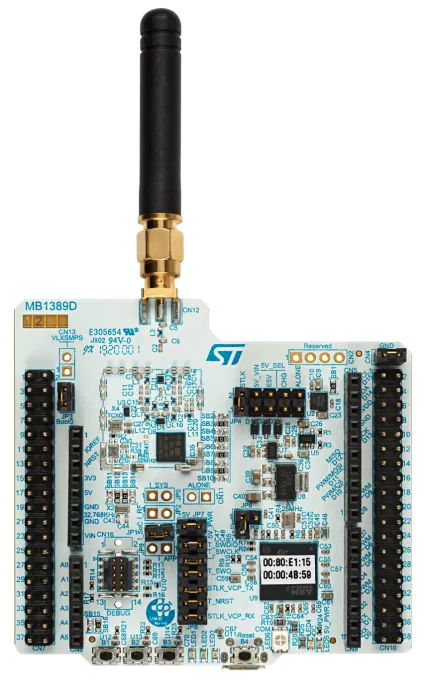
\includegraphics[width=5cm]{contents/chapter-2/stm32-wl55jc1.jpg}
	\caption{\textit{Development Board} STM32 Nucleo-WL55JC1}
	\label{Fig: STM32 Nucleo-WL55JC1}
\end{figure}

Perangkat ini sudah terintegrasi dengan STLINK-V3E, sehingga tidak dibutuhkan perangkat tambahan untuk memrogram dan melakukan \textit{debugging} pada perangkat \cite{STMicroelectronics2022}. Selain itu, perangkat ini juga mendukung penggunaan \textit{expansion board} Arduino dan ST morpho. \textit{Development board} STM32 Nucleo-WL55JC1 ditunjukan oleh Gambar \ref{Fig: STM32 Nucleo-WL55JC1}.

Mikrokontroler STM32WL55 memiliki \textit{clock speed} 48 MHz jika dibandingkan dengan Arduino Mega yang hanya 16 MHz. Selain itu, STM32WL55 memiliki SRAM dengan kapasitas 64 KB atau delapan kali lipat dari yang dimiliki oleh Arduino Mega \cite{STMicroelectronics2022b}.

Karena performa tinggi dengan konsumsi daya rendah, maka digunakan mikrokontroler STM32WL55. Selain itu, STM32 juga memiliki komunitas yang tidak kalah luas dengan komunitas Arduino dan ESP-32.

\subsection{Modul GNSS Teseo LIV3FL}
\subsection{Antena GPS }
\subsection{Modul LoRa(?)}
\chapter{METODE TUGAS AKHIR}

\section{Alat dan Bahan Tugas Akhir}
Dalam penelitian ini digunakan beberapa perangkat keras dan perangkat lunak. Perangkat keras yang digunakan dalam penelitian ini adalah sebagai berikut
\begin{enumerate}
	\item Apple MacBook Pro dengan prosesor Apple M1 Pro 16-\textit{core} dan memori terpadu 16 GB menggunakan sistem operasi macOS Ventura
	\item STM32 Nucleo-WL55JC1 berbasis ARM Cortex-M0 dan ARM Cortex-M4
	\item Modul GNSS Teseo LIV3FL
	\item Modul antena Taoglas xxxx
	\item Kabel \textit{jumper} untuk purwarupa alat
\end{enumerate}
Selanjutnya, perangkat lunak dan pustaka yang diunakan adalah sebagai berikut
\begin{enumerate}
	\item STM32CubeIDE sebagai IDE pada \textit{end node}
	\item Visual Studio Code sebagai IDE untuk merancang situs jaringan penampil
	\item Amazon Web Service untuk merancang API meliputi yang Lambda, API \textit{Gateway}, dan RDS
	\item MySQL sebagai basis data untuk pengolahan data
	\item Postman untuk menguji API yang telah dirancang
\end{enumerate}

\section{Alur Tugas Akhir}

\section{Studi Literatur}

\section{Analisis Kebutuhan Sistem}

\section{Perancangan \textit{End Node}}

\section{Perancangan API dan Basis Data}

\section{Perancangan Web Penampil}
\chapter{HASIL DAN PEMBAHASAN}

\section{Persiapan Pengujian}
Untuk mengevaluasi hasil penelitian maka perlu dilakukan uji coba untuk meninjau performa dari sistem yang telah dirancang. Pengujian hasil penelitian akan dibagi menjadi empat tahapan berbeda, yaitu:

\begin{enumerate}
	\item Pengujian daya rendah untuk meninjau bagaimana performa sistem ketika mode daya rendah pada modul Teseo-LIV3FL diaktifkan. Algoritma daya rendah yang digunakan adalah \textit{cyclic periodic mode}.
	\item Pengujian \textit{Geofencing} dilakukan untuk melihat bagaimana performa algoritma \textit{geofencing} ketika sistem berada di luar dan di dalam lingkungan Universitas Gadjah Mada.
	\item Pengujian \textit{rapid static survey} akan menguji performa modul Teseo-LIV3FL dalam keadaan diam selama satu jam dengan empat skenario berbeda.
	\item Pengujian di Bus Trans Gadjah Mada dilakukan untuk meninjau performa sistem ketika digunakan di dalam Bus Trans Gadjah Mada.
\end{enumerate}

Sebelum dilakukan pengujian perlu dilakukan perancangan purwarupa sistem yang meliputi perangkat keras dan perangkat lunak (\textit{firmware}) terlebih dahulu. Bagian perangkat keras terdiri dari modul Teseo-LIV3FL dan antena Abracon APARM1804-SG3. Modul Teseo-LIV3FL dihubungkan dengan \textit{development board} STM32 Nucleo-WL55JC1 dengan komunikasi UART.

Setelah purwarupa sistem berhasil dirakit, maka langkah selanjutnya adalah menghubungkan \textit{development board} ke komputer dengan menggunakan kabel USB dan mengatur \textit{baud rate} sebesar 115200 Bps. Aplikasi yang digunakan untuk melakukan \textit{logging} dan perekaman data adalah CoolTerm. Selanjutnya, sistem akan diuji coba dengan menggunakan empat tahapan pengujian yang telah disebutkan sebelumnya untuk mengevaluasi performa dari sistem yang telah dirancang dan dirakit.

\section{Pengujian Daya Rendah}
Pada pengujian daya rendah, konfigurasi \textit{common ground} digunakan saat merangkai modul Teseo-LIV3FL dan multimeter agar keduanya dapat berbagi titik acuan yang sama. Hal ini memungkinkan pengukuran yang lebih akurat terhadap arus yang mengalir pada modul Teseo-LIV3FL. Untuk menghubungkan modul Teseo-LIV3FL dengan komputer, digunakan perangkat USB \textit{to} TTL \textit{converter} yang juga berfungsi sebagai sumber arus untuk menyalakan modul Teseo-LIV3FL. Gambar \ref{Fig: low-power-connected} menunjukkan contoh dari modul Teseo-LIV3FL yang sudah terhubung dengan multimeter dan siap untuk dilakukan pengujian daya rendah.

\begin{figure}[H]
	\centering
	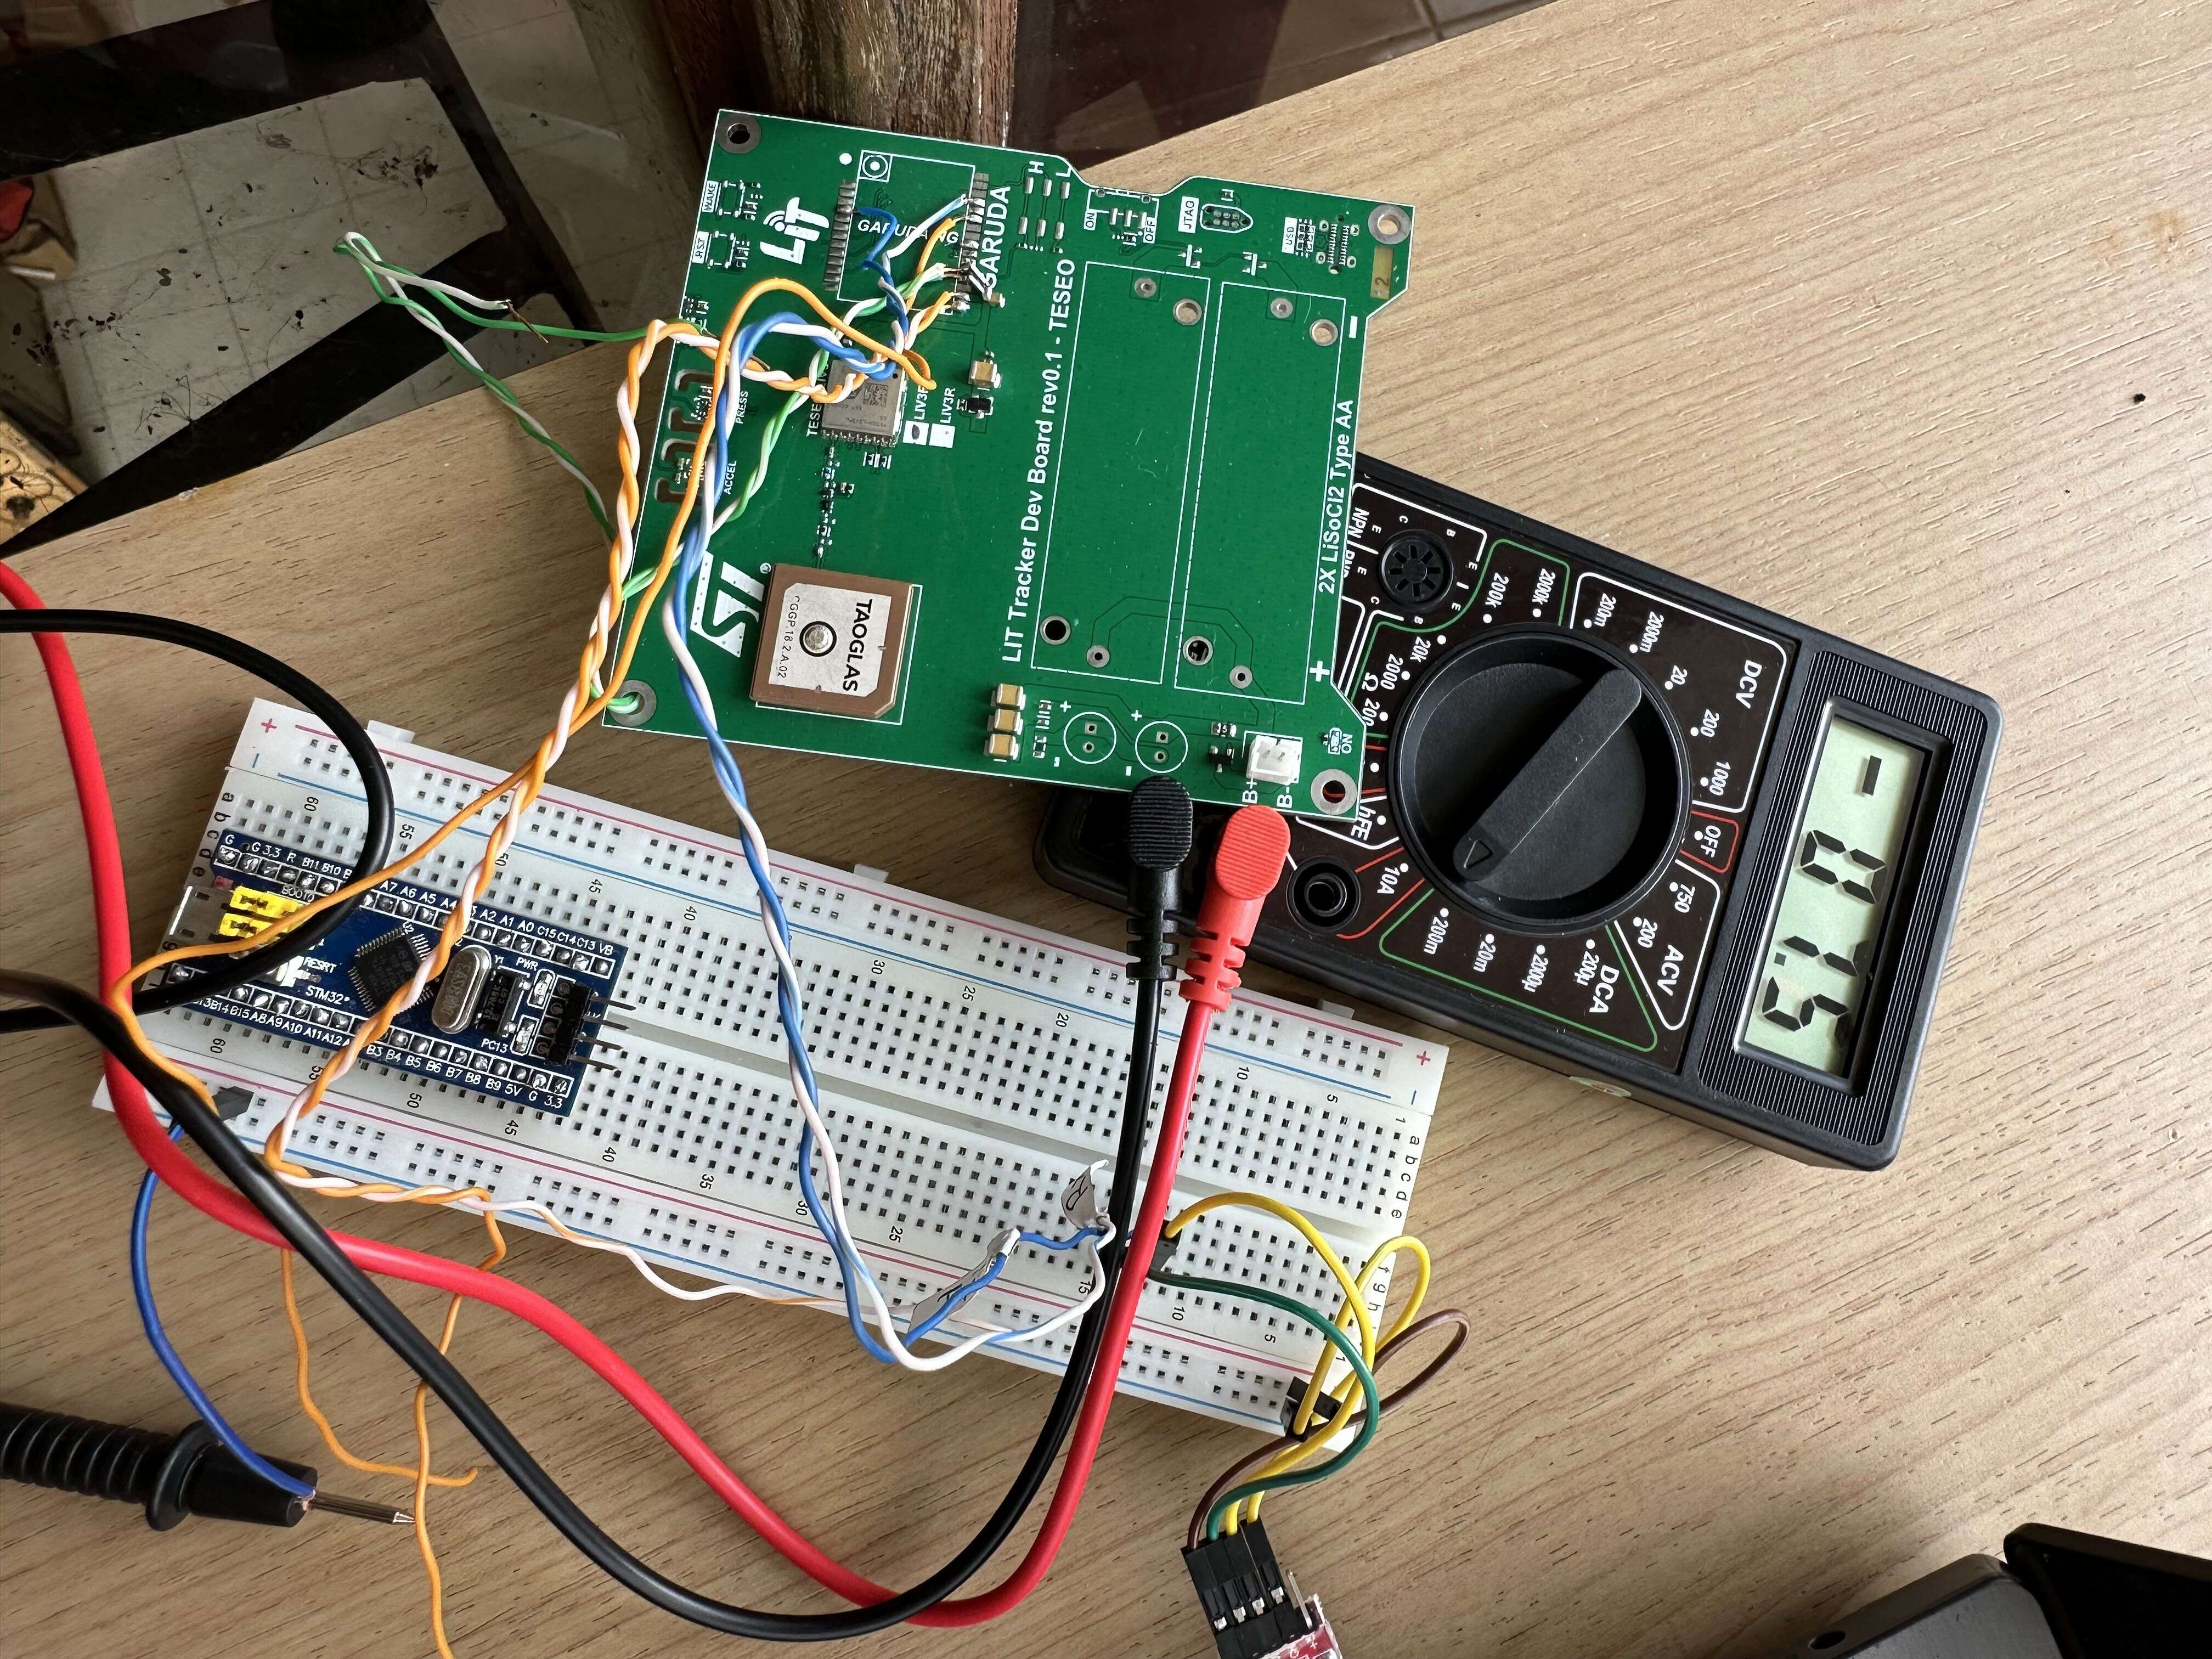
\includegraphics[width=10cm]{contents/chapter-4/low-power.jpg}
	\caption{Modul GNSS yang telah Terangkai dengan Multimeter}
	\label{Fig: low-power-connected}
\end{figure}

Algoritma daya rendah yang digunakan pada pengujian ini adalah mode periodik. Mode periodik pada modul Teseo-LIV3FL memungkinkan modul tersebut berada dalam mode akuisisi dalam waktu tertentu hingga mendapatkan posisi \textit{fix}. Setelah modul Teseo-LIV3FL mendapatkan posisi \textit{fix}, maka modul tersebut akan beralih ke mode \textit{stand by} untuk menghemat daya. Kemudian, setelah periode waktu tertentu, modul Teseo-LIV3FL akan kembali masuk ke mode akuisisi untuk mendapatkan posisi \textit{fix} kembali. Jika modul Teseo-LIV3FL tidak dapat mendapatkan posisi \textit{fix}, maka modul tersebut akan tetap masuk ke mode \textit{stand by} dan mencoba untuk mendapatkan posisi \textit{fix} kembali setelah periode waktu tertentu. Algoritma daya rendah ini sangat penting dalam memastikan modul Teseo-LIV3FL mampu beroperasi dengan menggunakan daya yang sangat kecil namun tetap dapat mendapatkan posisi \textit{fix} dengan akurasi yang cukup baik.

Perintah \$PSTMLOWPOWERONOFF digunakan untuk mengendalikan mode daya rendah pada modul Teseo-LIV3FL. Perintah ini menerima empat belas argumen dengan rincian tertentu untuk setiap mode daya rendah yang diaktifkan. Pada mode adaptif, empat argumen kedua hingga kelima digunakan untuk mengatur ambang batas untuk mode daya rendah, sedangkan pada mode \textit{cyclic}, digunakan dua argumen selanjutnya. Pada mode periodik, delapan argumen terakhir digunakan untuk mengatur frekuensi dan waktu mode daya rendah. Pada pengujian ini, digunakan mode daya rendah periodik, sehingga argumen kedua hingga ketujuh harus diisi dengan angka nol. Perintah yang dikirimkan pada pengujian ini adalah sebagai berikut:

\begin{verbatim}
	$PSTMLOWPOWERONOFF,1,0,0,0,0,0,0,3,60,1,1,1,60,30
\end{verbatim}

Perintah di atas akan mengaktifkan mode daya rendah periodik pada modul Teseo-LIV3FL dengan waktu \textit{stand by} selama satu menit setelah mendapatkan tiga posisi \textit{fix}. Artinya, setelah modul menerima tiga posisi \textit{fix}, maka modul akan masuk ke mode daya rendah dan hanya akan mengambil posisi setiap satu menit. Selain itu, modul juga akan menuju mode \textit{stand by} selama tiga puluh detik jika tidak dapat mendapatkan posisi \textit{fix} selama satu menit. Detail argumen yang digunakan pada pengujian ini dapat dilihat pada Tabel 4.1.

\begin{longtblr}[caption = {Argumen pada Perintah \$PSTMLOWPOWERONOFF}]{
		width = \linewidth,
		colspec = {Q[285]Q[48]Q[608]},
		row{1} = {c},
		row{3} = {c},
		row{5} = {c},
		row{6} = {c},
		row{7} = {c},
		row{8} = {c},
		row{10} = {c},
		row{11} = {c},
		cell{2}{1} = {c},
		cell{2}{2} = {c},
		cell{3}{1} = {c=3}{0.941\linewidth},
		cell{4}{1} = {c},
		cell{4}{2} = {c},
		cell{4}{3} = {r=4}{},
		cell{8}{1} = {c=3}{0.941\linewidth},
		cell{9}{1} = {c},
		cell{9}{2} = {c},
		cell{9}{3} = {r=2}{},
		cell{11}{1} = {c=3}{0.941\linewidth},
		cell{12}{1} = {c},
		cell{12}{2} = {c},
		cell{13}{1} = {c},
		cell{13}{2} = {c},
		cell{14}{1} = {c},
		cell{14}{2} = {c},
		cell{15}{1} = {c},
		cell{15}{2} = {c},
		cell{16}{1} = {c},
		cell{16}{2} = {c},
		cell{17}{1} = {c},
		cell{17}{2} = {c},
		cell{18}{1} = {c},
		cell{18}{2} = {c},
		hline{1-4,8-9,11-12} = {-}{},
	}
	\textbf{Argumen}                               & \textbf{Nilai} & \textbf{Keterangan}                                                                                                                      \\
	Menyalakan atau mematikan mode daya rendah     & 1              & Mode daya rendah dinyalakan                                                                                                              \\
	Mode Adaptif                                   &               0 &                                                                                                                                          \\
	\textit{Constellation mask}                    & 0              & Mode adaptif tidak digunakan.                                                                                                            \\
	Batas EHPE                            &               0 &                                                                                                                                          \\
	Satelit maksimum                               &               0 &                                                                                                                                          \\
	Perpindahan konstelasi otomatis                &         0       &                                                                                                                                          \\
	Mode \textit{cyclic}                           &           0     &                                                                                                                                          \\
	Menyalakan atau mematikan \textit{duty cycle} & 0              & Mode \textit{cyclic} tidak digunakan.\\
	Periode \textit{duty cycle}                    &         0       &                                                                                                                                          \\
	Mode periodik                                  &                &                                                                                                                                          \\
	Mode periodik                                  & 3              & Mode periodik \textit{stand by}                                                                                                          \\
	FixPeriod                                      & 60             & Modul akan memasuki mode~\textit{stand by} selama enam puluh detik setelah mendapat posisi \textit{fix}                                \\
	FixOnTime                                      & 3              & Memasuki mode \textit{stand by~setelah mendapatkan tiga posisi \textit{fix}}                                                             \\
	Penyegaran ephemeris                           & 1              & Penyegaran ephemeris diaktifkan                                                                                                          \\
	Kalibrasi RTC                                  & 1              & Kalibrasi RTC diaktifkan                                                                                                                 \\
	NoFixCnt                                       & 60             & Modul akan memasuki mode \textit{stand by} jika tidak bisa mendapatkan posisi \textit{fix~setelah enam puluh detik (\textit{fix loss)}} \\
	NoFixOff                                       & 30             & Modul memasuki \textit{stand by} selama tiga puluh detik setelah \textit{fix loss}\\
	\hline                                                      
\end{longtblr}

Hasil pengukuran menunjukkan bahwa arus yang mengalir pada modul Teseo-LIV3FL adalah sebesar 46,3 mA. Namun, hal yang menarik adalah nilai arus yang diukur jauh lebih kecil daripada nilai arus yang tertera pada \textit{datasheet}, yang mencapai 65 mA. Dalam mode \textit{stand by}, modul Teseo-LIV3FL berada dalam kondisi siap dan hanya menunggu untuk melakukan pencarian posisi kembali. Oleh karena itu, arus yang mengalir pada modul Teseo-LIV3FL sudah mendekati nilai \textit{datasheet} yang hanya 10 $\mu$A, yaitu sebesar 15 $\mu$A. Hal ini menunjukkan bahwa penggunaan mode daya rendah pada modul Teseo-LIV3FL dapat menurunkan konsumsi daya hingga lebih dari 4 kali lipat pada saat berada dalam mode akuisisi. Gambar \ref{Fig: low-power-result} menunjukkan hasil pengukuran multimeter ketika modul Teseo-LIV3FL berada dalam mode akuisisi (kiri) dan mode \textit{stand by} (kanan), yang menunjukkan perbedaan yang signifikan dalam tingkat konsumsi daya antara kedua mode tersebut.

\begin{figure}[H]
	\centering
	\captionsetup{justification=centering}
	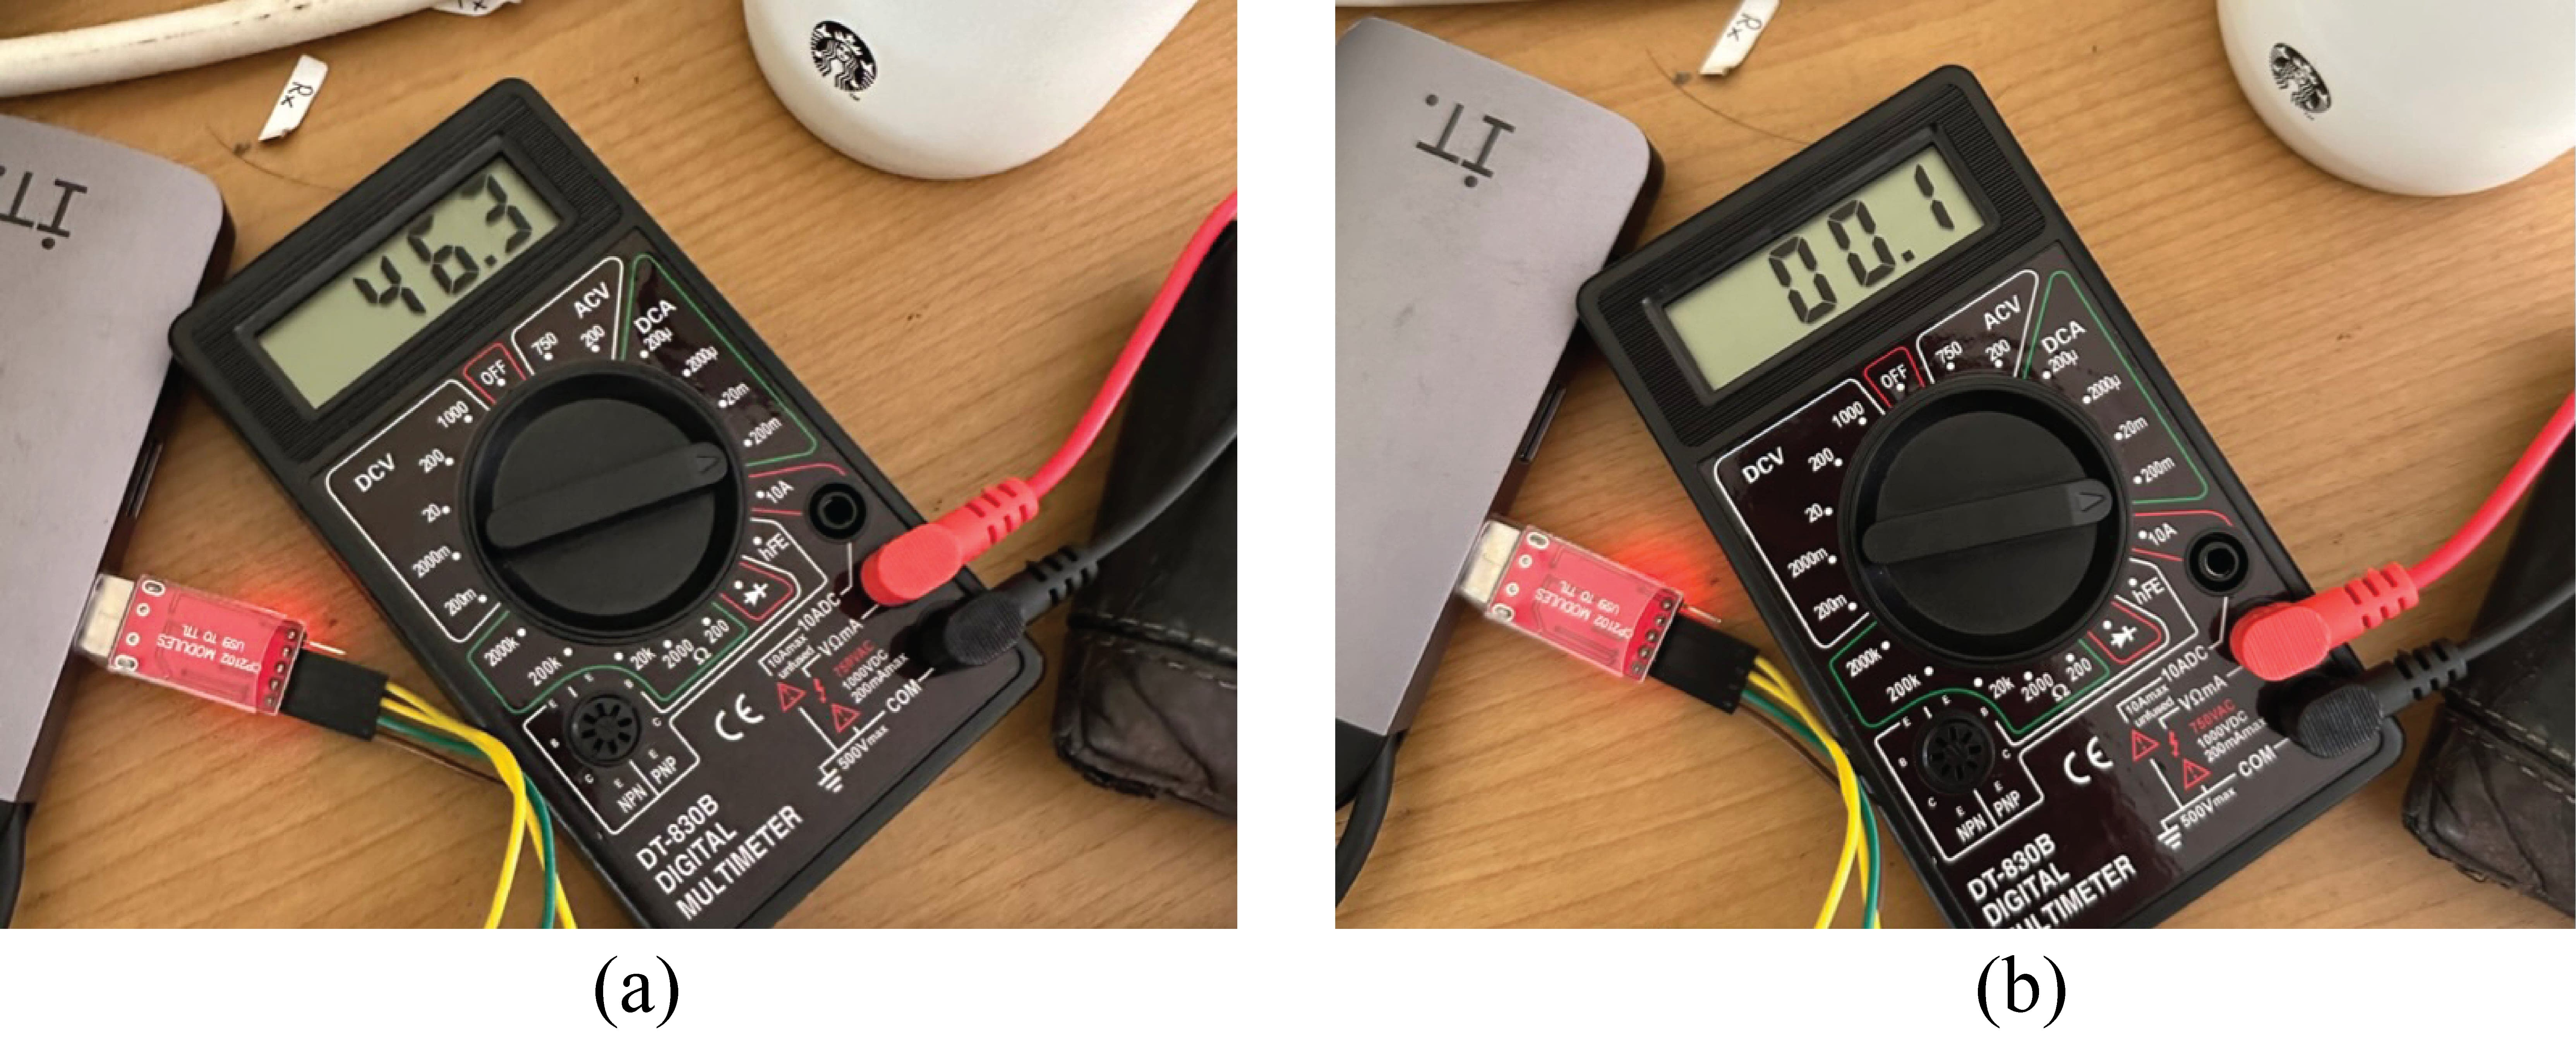
\includegraphics[width=14cm]{contents/chapter-4/low-power-result.jpg}
	\caption{Pembacaan Multimeter pada Mode Akuisisi (Kiri) dan Mode \textit{Stand By} (Kanan)}
	\label{Fig: low-power-result}
\end{figure}

\section{Pengujian \textit{Rapid Static Survey}}
Rapid Static Survey adalah pengujian yang dilakukan untuk meninjau performa modul GNSS dalam keadaan diam. Pengujian ini dapat dilakukan dalam rentang waktu lima belas menit s.d. dua jam \cite{lauer2019static}. Pengujian ini akan meninjau  dan presisi dari modul GNSS. Akurasi adalah tingkat kedekatan hasil pembacaan modul GNSS dengan posisi sebenarnya, sedangkan tingkat presisi menunjukan seberapa dekat hasil yang didapat dengan rata-rata dari seluruh sampel \cite{gnssca_apn029}.

Pada pengujian rapid static survey, modul Teseo-LIV3FL diletakan dalam empat skenario selama satu jam. Skenario tersebut meliputi \textit{basement}, dalam ruangan, ruangan semi terbuka, dan ruang terbuka. Pengujian setiap skenario dilakukan pada empat titik di lingkungan Universitas Gadjah Mada, yaitu:

\begin{enumerate}
	\item \textit{Basement} diwakili oleh tempat parkir bawah tanah milik Fakultas Ilmu Sosial dan Ilmu Politik.
	\item Ruangan tertutup diwakili oleh Lantai 5 Gedung SGLC Fakultas Teknik
	\item Ruang semi terbuka diwakili oleh Selasar Grha Sabha Pramana.
	\item Ruangan terbuka diwakili oleh Lapangan Pancasila
\end{enumerate}

Nilai HDOP (\textit{Horizontal Dilution of Precision}), VDOP (\textit{Vertical Dilution of Precision}), PDOP (\textit{Position Dilution of Precision}), dan MAD (\textit{Mean Absolute Deviation}) adalah parameter yang digunakan untuk mengevaluasi akurasi dan presisi dari pengukuran GNSS. Pada pengujian Rapid Static Survey, nilai-nilai HDOP, VDOP, PDOP, dan CEP akan diamati di setiap skenario dan titik pengujian. Hal ini akan memberikan informasi tentang seberapa akurat dan presisi posisi yang dihasilkan oleh modul Teseo-LIV3FL dalam berbagai kondisi lingkungan dan dapat membantu dalam mengevaluasi performa modul GNSS tersebut.

\subsection{Skenario \textit{Basement}}
Pengujian skenario \textit{basement} dilakukan dengan tujuan untuk memperoleh gambaran tentang performa modul Teseo-LIV3FL di dalam ruangan bawah tanah. Ruangan bawah tanah seringkali digunakan sebagai tempat parkir mobil, gudang, atau ruang penyimpanan yang berada di bawah gedung. Karena letaknya yang berada di bawah tanah, maka akses isyarat satelit GNSS menjadi terbatas. Dalam pengujian ini, modul Teseo-LIV3FL diletakkan di tempat parkir bawah tanah yang berada di bawah gedung empat lantai dengan struktur beton. Pengujian dilakukan pada lingkungan yang sangat tertutup dan minim sinar matahari. Terdapat beberapa area terbuka kecil yang memungkinkan sedikit sinar matahari untuk masuk. Gambar \ref{Fig: basement-keadaan} menunjukkan kondisi lingkungan saat pengujian skenario \textit{basement}.

\begin{figure}[H]
	\centering
	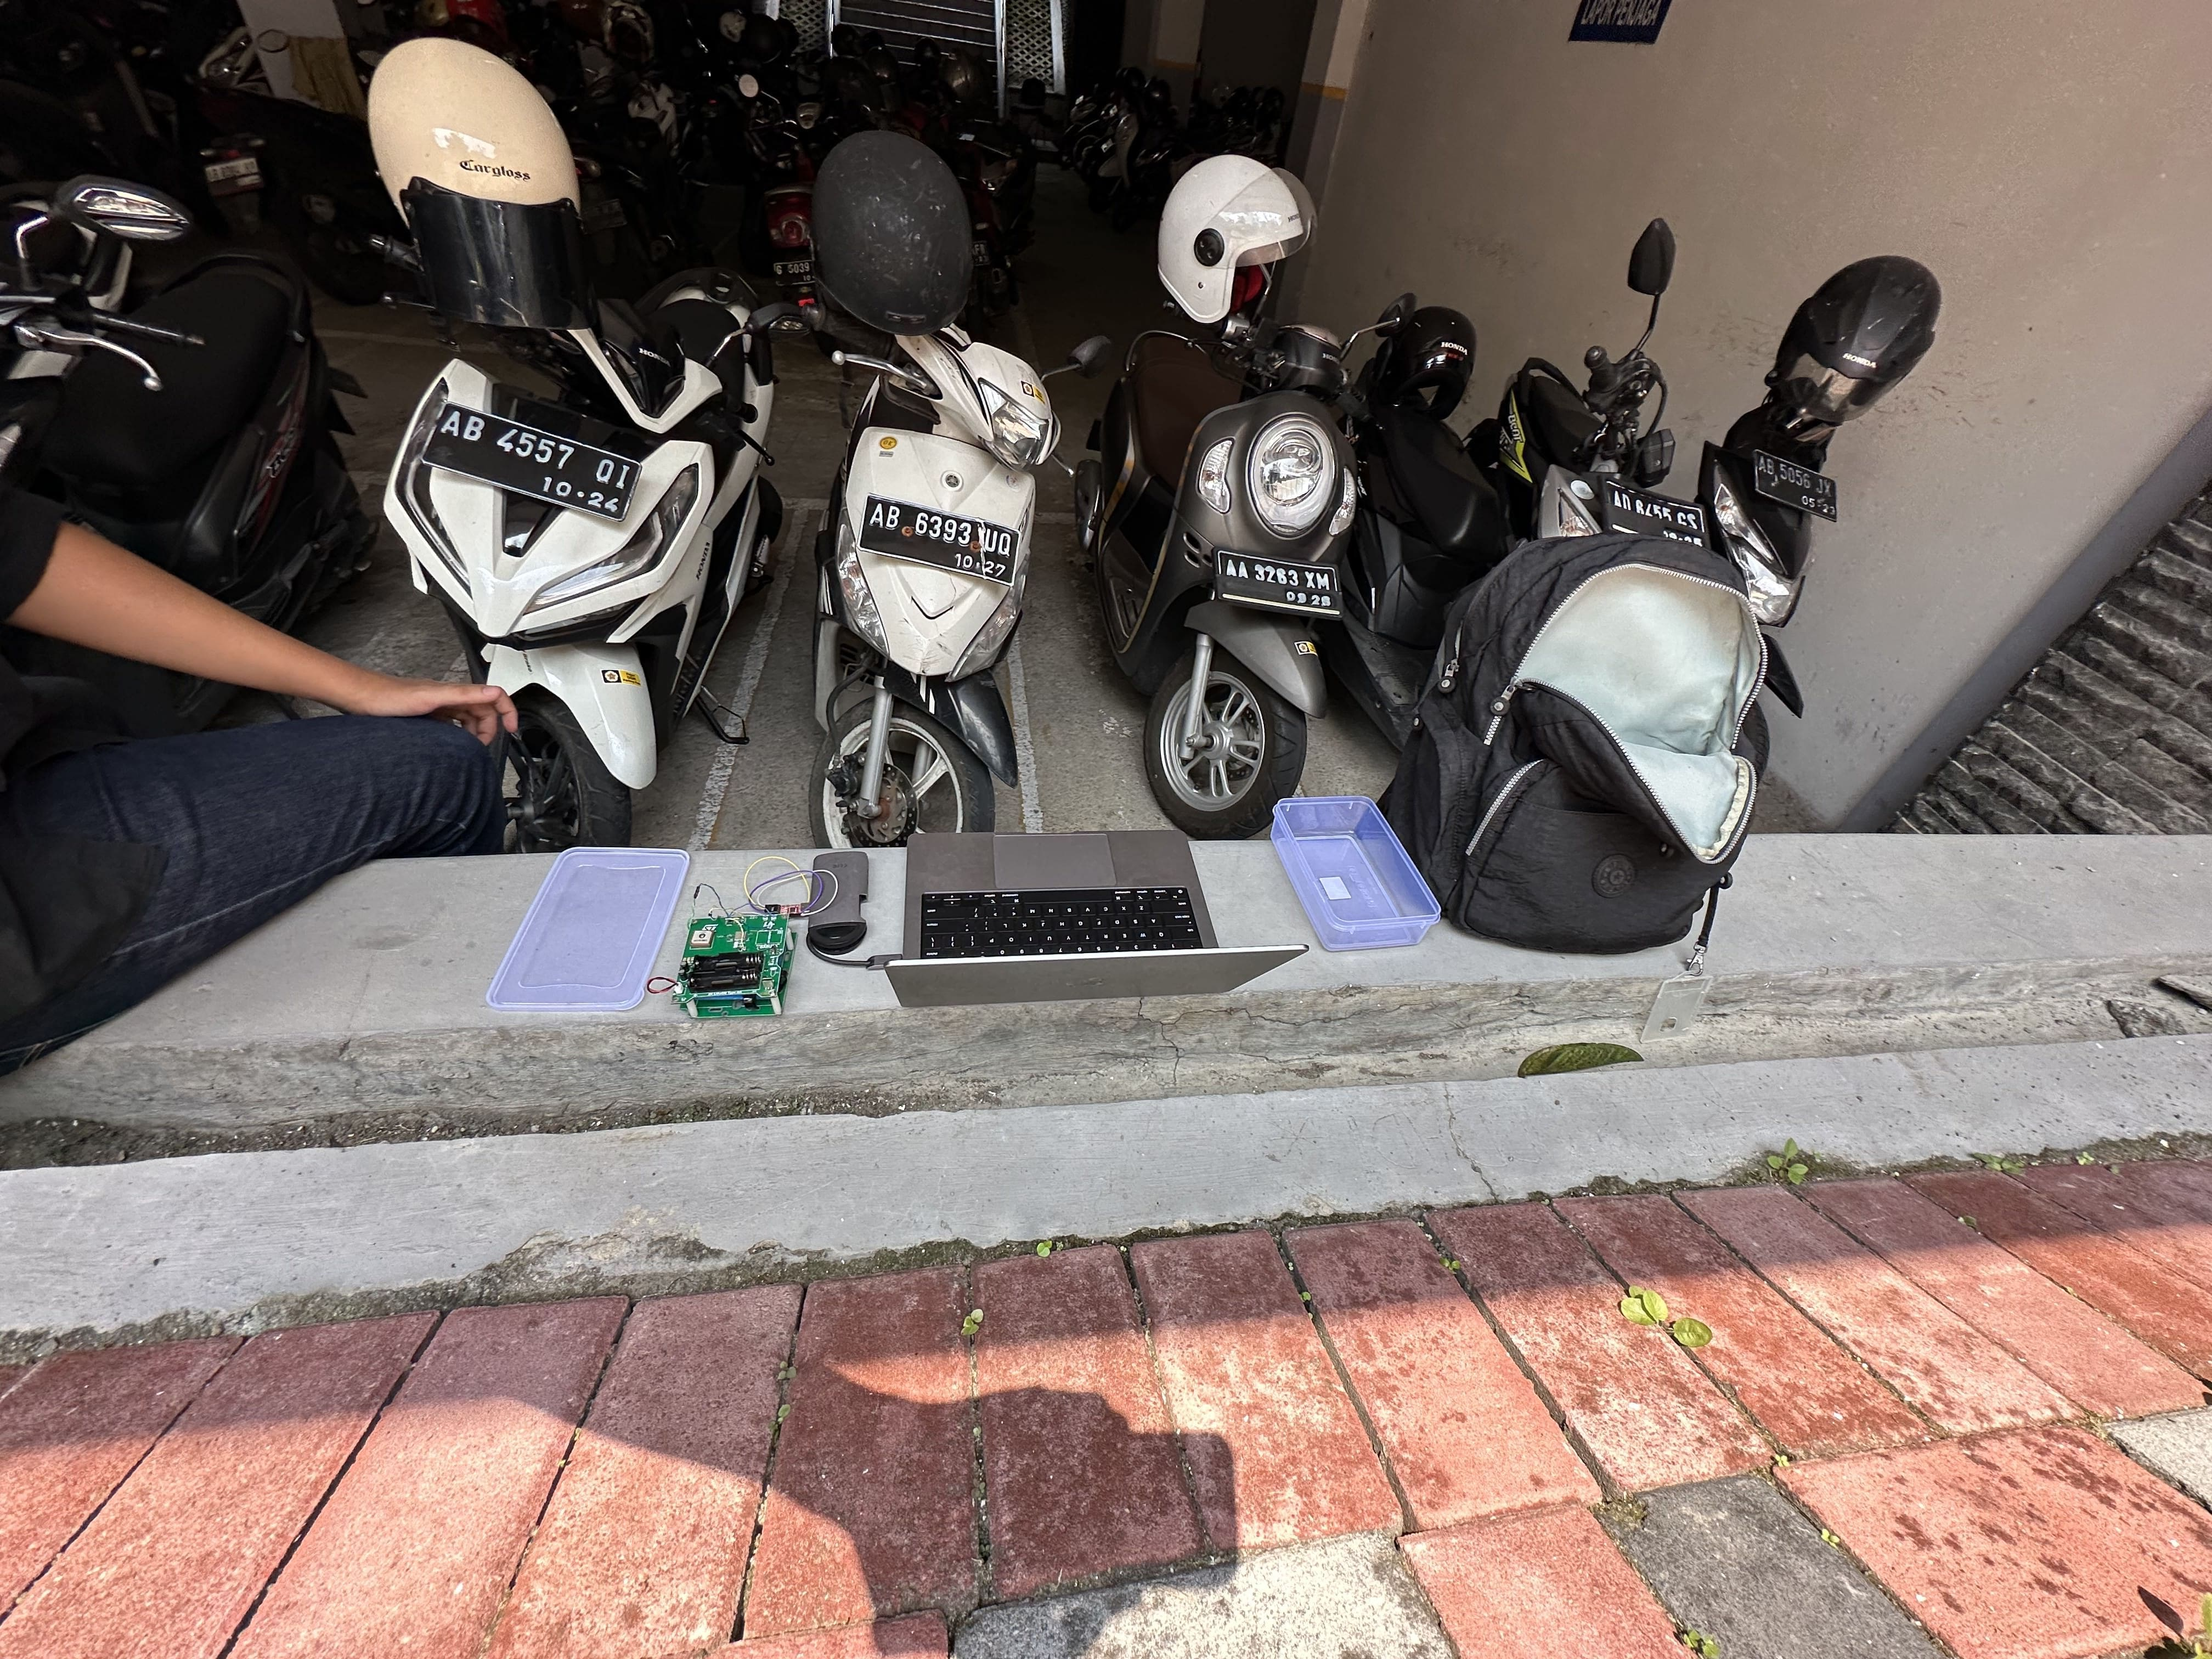
\includegraphics[width=10cm]{contents/chapter-4/1-skenario-basement/keadaan.jpg}
	\caption{Pengujian Skenario \textit{Basement}}
	\label{Fig: basement-keadaan}
\end{figure}

\begin{figure}[H]
	\centering
	\begin{adjustbox}{width=\textwidth}
		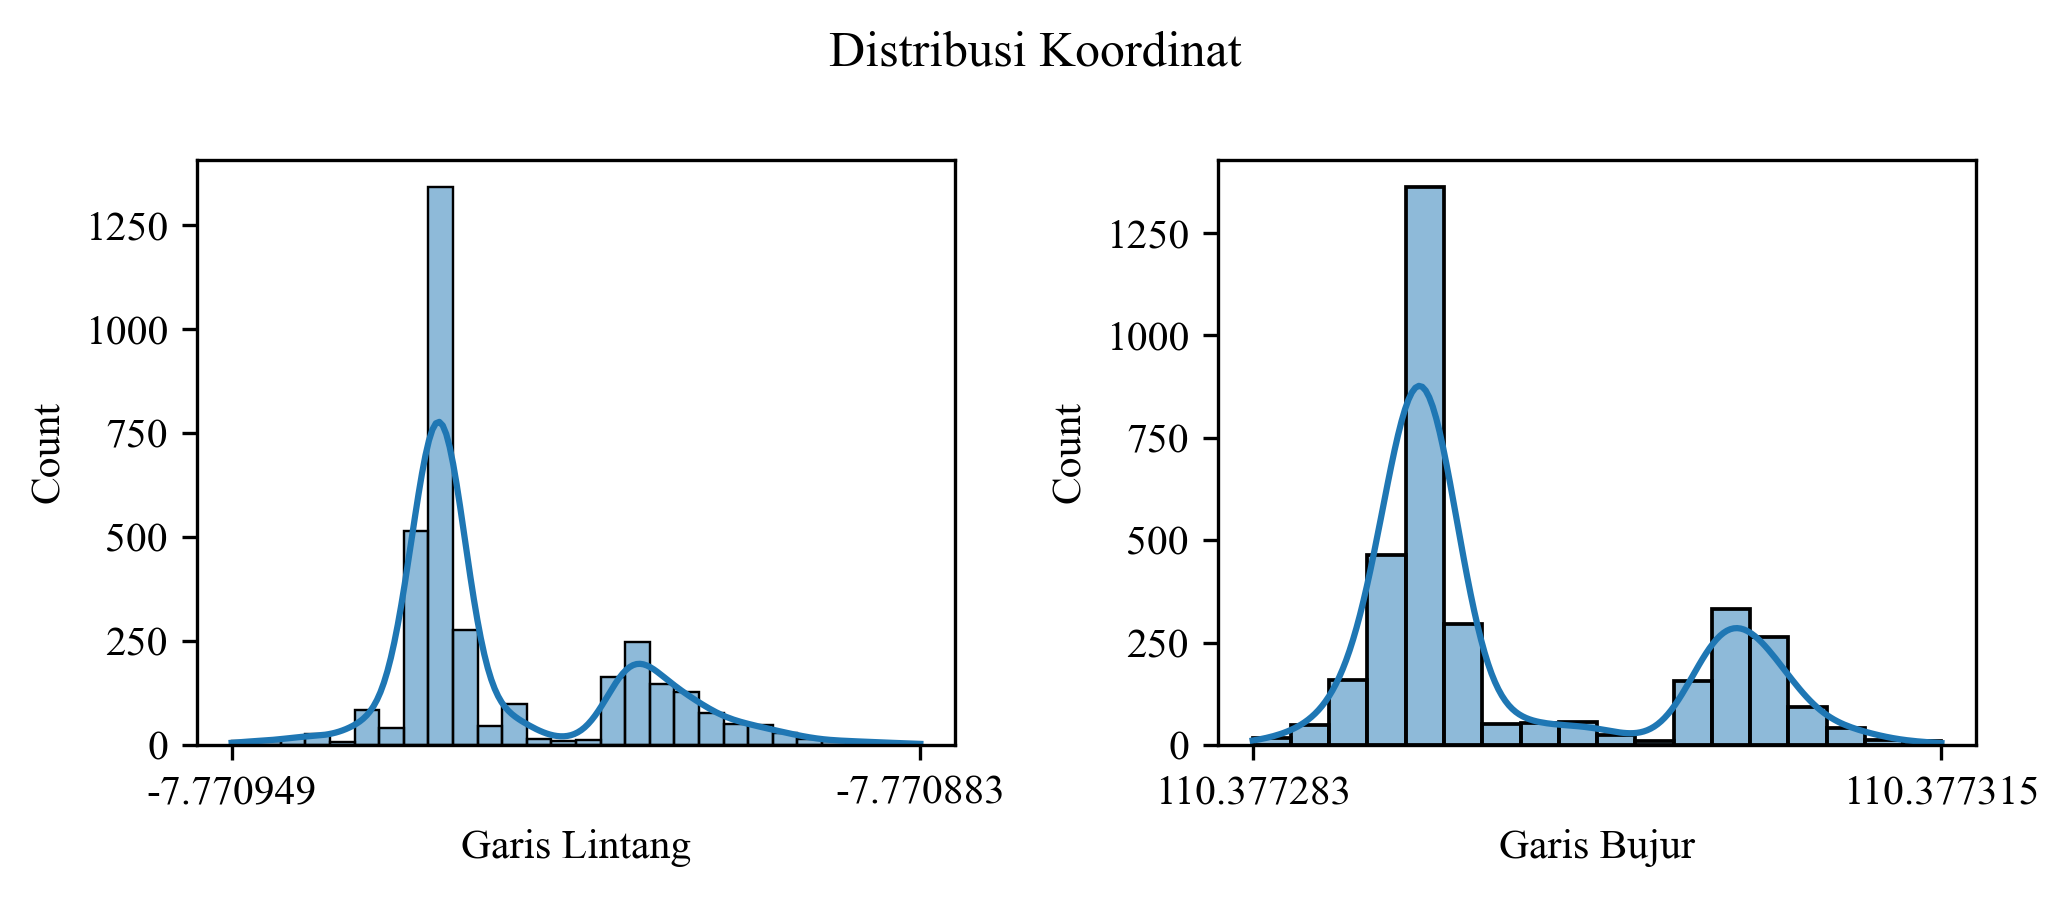
\includegraphics{contents/chapter-4/1-skenario-basement/distribution.png}
	\end{adjustbox}
	\caption{Distribusi Data Koordinat Skenario \textit{Basement}}
	\label{Fig:basement-distribution}
\end{figure}

Grafik persebaran distribusi koordinat pada Gambar \ref{Fig:basement-distribution} menunjukkan bahwa koordinat garis lintang memiliki rentang tersebar antara -7,769728 hingga -7,768525 sedangkan untuk garis bujur memiliki rentang tersebar antara 110,379841 hingga 110,380314. Modus dari kedua koordinat berada pada titik -7.769356 dan 110.379952.Terlihat bahwa kedua koordinat tidak terdistribusi secara normal sehingga tidak memungkinkan untuk melakukan analisis CEP. Oleh karena itu, akan dilakukan analisis MAD.

\begin{table}[H]
	\caption{Hasil Pengujian Skenario \textit{Basement}}
	\vspace{0.5em}
	\centering
	\begin{tabular}{ccccc}
		\hline
		& \textbf{Minima} & \textbf{Maxima} & \textbf{Rata-rata} & \textbf{Standar Deviasi}\\
		\hline 
		HDOP & 1,80 & 26,80 & 8,27 & 5,36\\
		PDOP & 2,80 & 39,30 & 10,67 & 7,30\\
		VDOP & 2,00 & 28,80 & 8,27 & 5,36\\
		Jumlah Satelit & 5 & 12 & 7,60 & 1,27\\
		\hline
		\textbf{MAD-x (m)} & & \multicolumn{2}{c}{\centering 18,89} & \\
		\hline
		\textbf{MAD-y (m)} & & \multicolumn{2}{c}{\centering 14,99} & \\
		\hline
		\textbf{MAD (m)} & & \multicolumn{2}{c}{\centering 24,11} & \\
		\hline
	\end{tabular}
	\label{Tab: basement-table}
\end{table}

Pada skenario \textit{basement}, hasil pengukuran modul Teseo-LIV3FL menunjukkan hasil yang kurang akurat. Hal ini terlihat pada data yang dicatat pada Gambar \ref{Fig: basement-sats_dop}, yang menunjukkan adanya lonjakan nilai DOP. Selain itu, nilai maksimum PDOP yang dicatat pada Tabel \ref{Tab: basement-table} adalah sebesar 39,30. Nilai yang sangat tinggi ini mengindikasikan bahwa persebaran satelit di langit tidak mencakup seluruh lingkaran, seperti terlihat pada \textit{sky plot} pada Gambar \ref{Fig: basement-skyplot}. \textit{Sky plot} tersebut memperlihatkan bahwa persebaran satelit hanya mencakup setengah bagian dari lingkaran, sehingga dapat mempengaruhi akurasi keseluruhan dari hasil pengukuran modul Teseo-LIV3FL. Analisis MAD menunjukan bahwa tingkat kepresisian modul Teseo-LIV3Fl pada skenario \textit{basement} adalah 18,89 meter pada sumbu garis lintang, 14,99 pada sumbu garis bujur, dan 24,11 meter secara keseluruhan.

\begin{figure}[H]
	\centering
	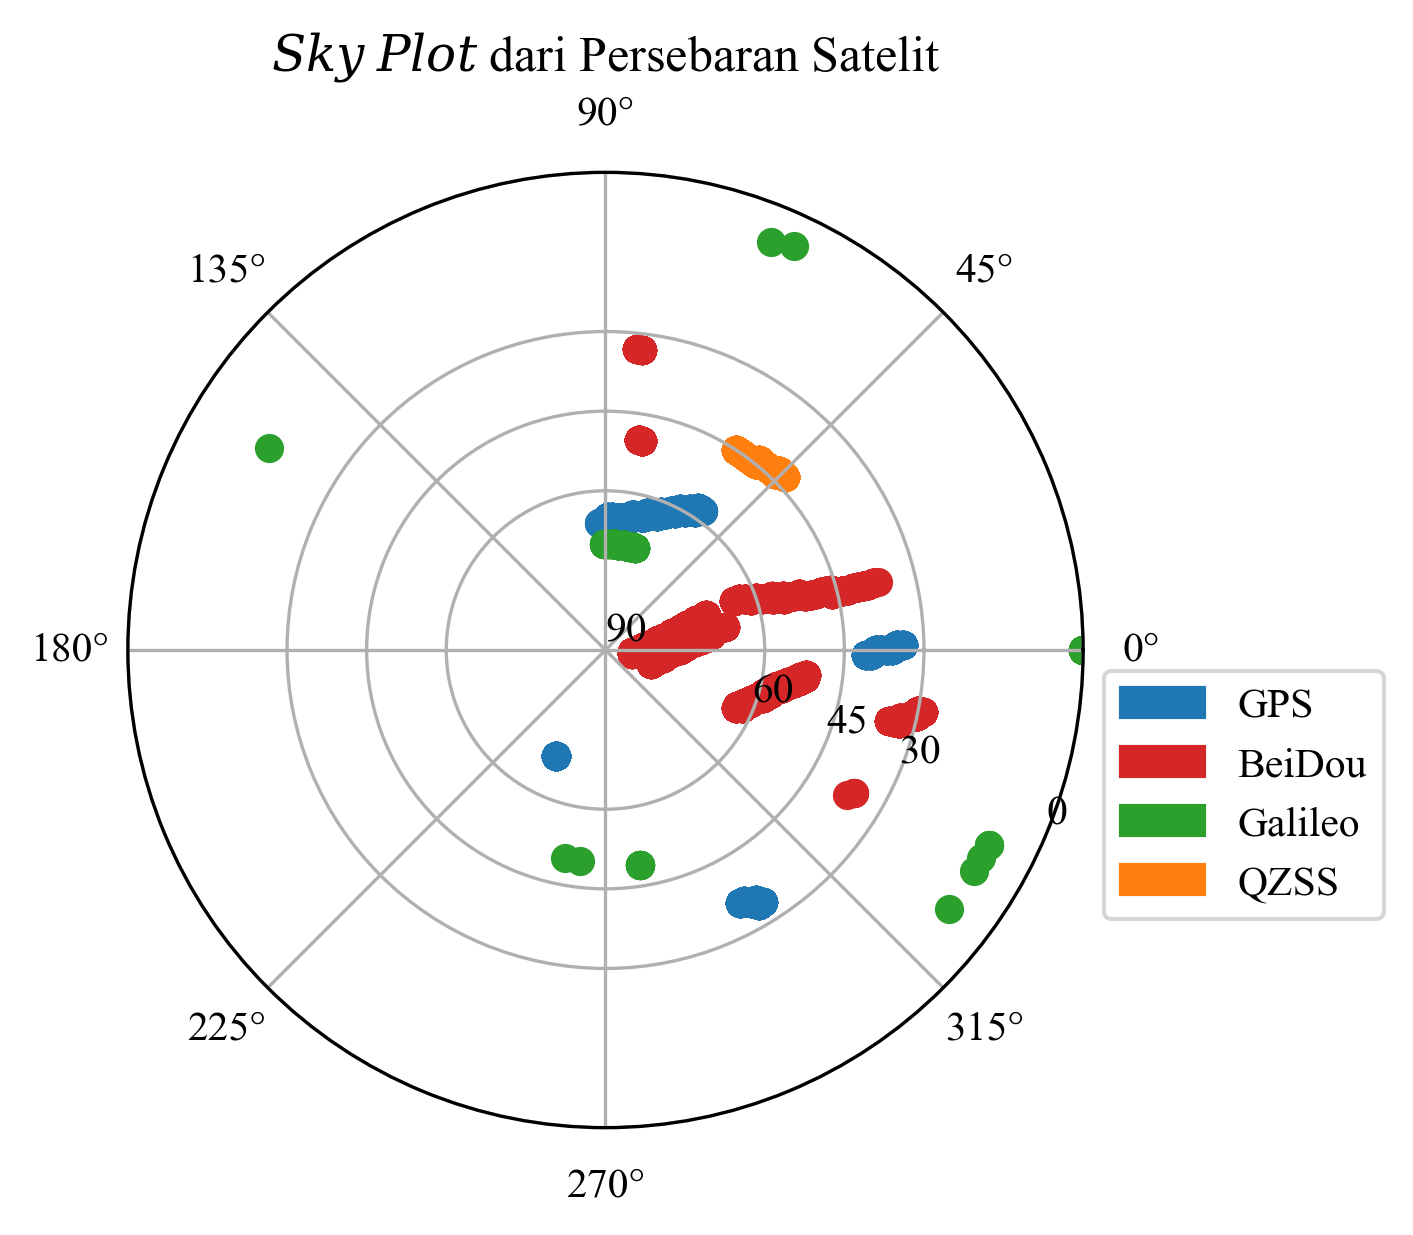
\includegraphics[width=11cm]{contents/chapter-4/1-skenario-basement/skyplot.png}
	\caption{\textit{Sky Plot} Pengujian Skenario \textit{Basement}}
	\label{Fig: basement-skyplot}
\end{figure}

\begin{figure}[H]
	\centering
	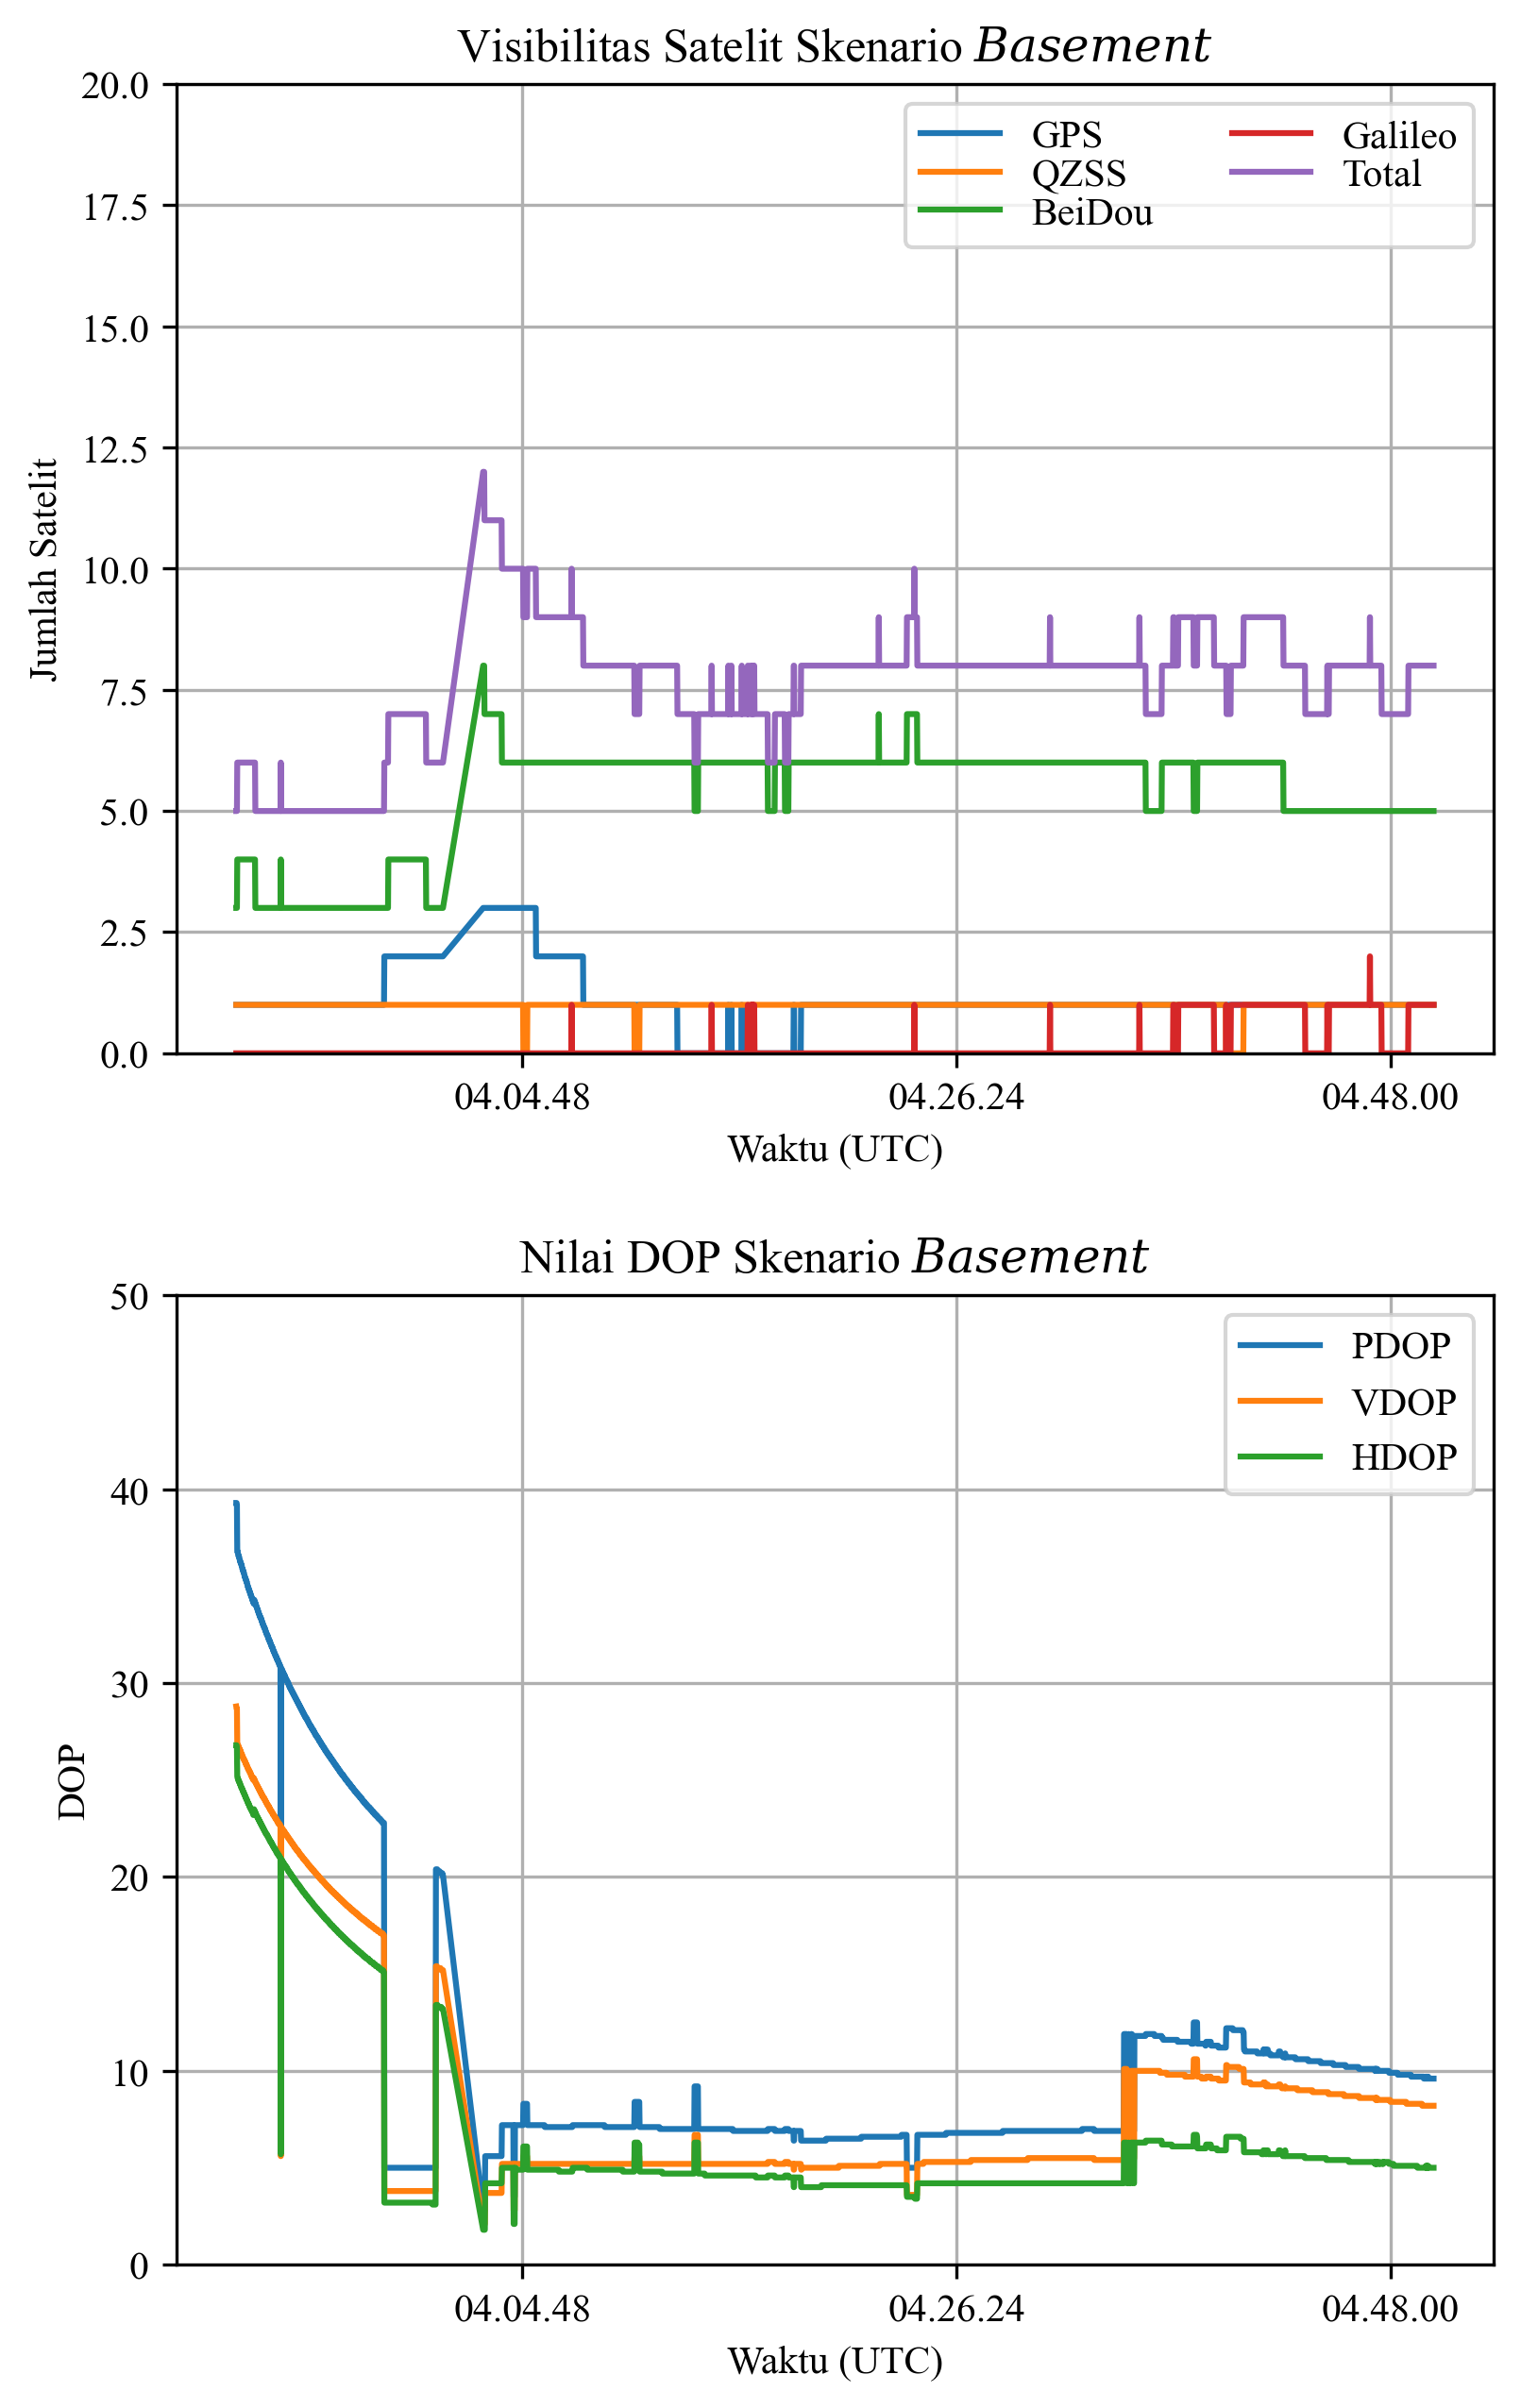
\includegraphics[width=12cm]{contents/chapter-4/1-skenario-basement/sats_dop.png}
	\caption{DOP dan Visibilitas Satelit Pengujian Skenario \textit{Basement}}
	\label{Fig: basement-sats_dop}
\end{figure}

Meskipun modul Teseo-LIV3FL tertutup oleh struktur beton, modul tetap mampu menangkap isyarat dari keempat konstelasi Teseo-LIV3FL yang telah diatur. Dari hasil pengujian, terlihat bahwa konstelasi dengan jumlah satelit paling banyak adalah BeiDou milik Republik Rakyat Tiongkok. Namun, terjadi lonjakan nilai DOP pada awal pengujian saat jumlah satelit paling rendah. Hal ini menunjukkan bahwa jumlah satelit yang rendah akan meningkatkan ketiga nilai DOP, yang pada akhirnya akan menurunkan akurasi dari hasil pembacaan modul Teseo-LIV3FL.

Angka 24,11 meter pada hasil analisis MAD menunjukan tingkat presisi masih rendah, tetapi nilai rata-rata HDOP yang menunjukan angka 8,27 tetap menunjukan bahwa hasil pengukuran posisi masih layak untuk digunakan. Perlu diingat bahwa pengujian ini dilakukan di lingkungan yang sangat sulit, yaitu ruangan bawah tanah dengan struktur beton yang menutupi sinyal dari satelit. Selain itu, terdapat sedikit bagian terbuka yang memungkinkan sinar matahari untuk memasuki ruangan. Meskipun demikian, pengujian ini menunjukan bahwa modul GNSS masih dapat digunakan untuk mendapatkan posisi \textit{fix} dalam kondisi lingkungan yang sulit seperti ini.

\subsection{Skenario Dalam Ruangan}
Pengujian skenario dilakukan di dalam ruangan tertutup pada lantai 5 Gedung SGLC Fakultas Teknik. Ruangan pengujian dilengkapi dengan jendela besar yang memungkinkan lebih banyak sinar matahari untuk masuk ke dalam ruangan, sehingga menghasilkan kondisi lingkungan yang cukup berbeda dengan pengujian skenario di \textit{basement}. Gambar \ref{Fig: indoor-keadaan} menunjukkan pengujian skenario dalam ruangan yang dilakukan pada penelitian ini.

\begin{figure}[H]
	\centering
	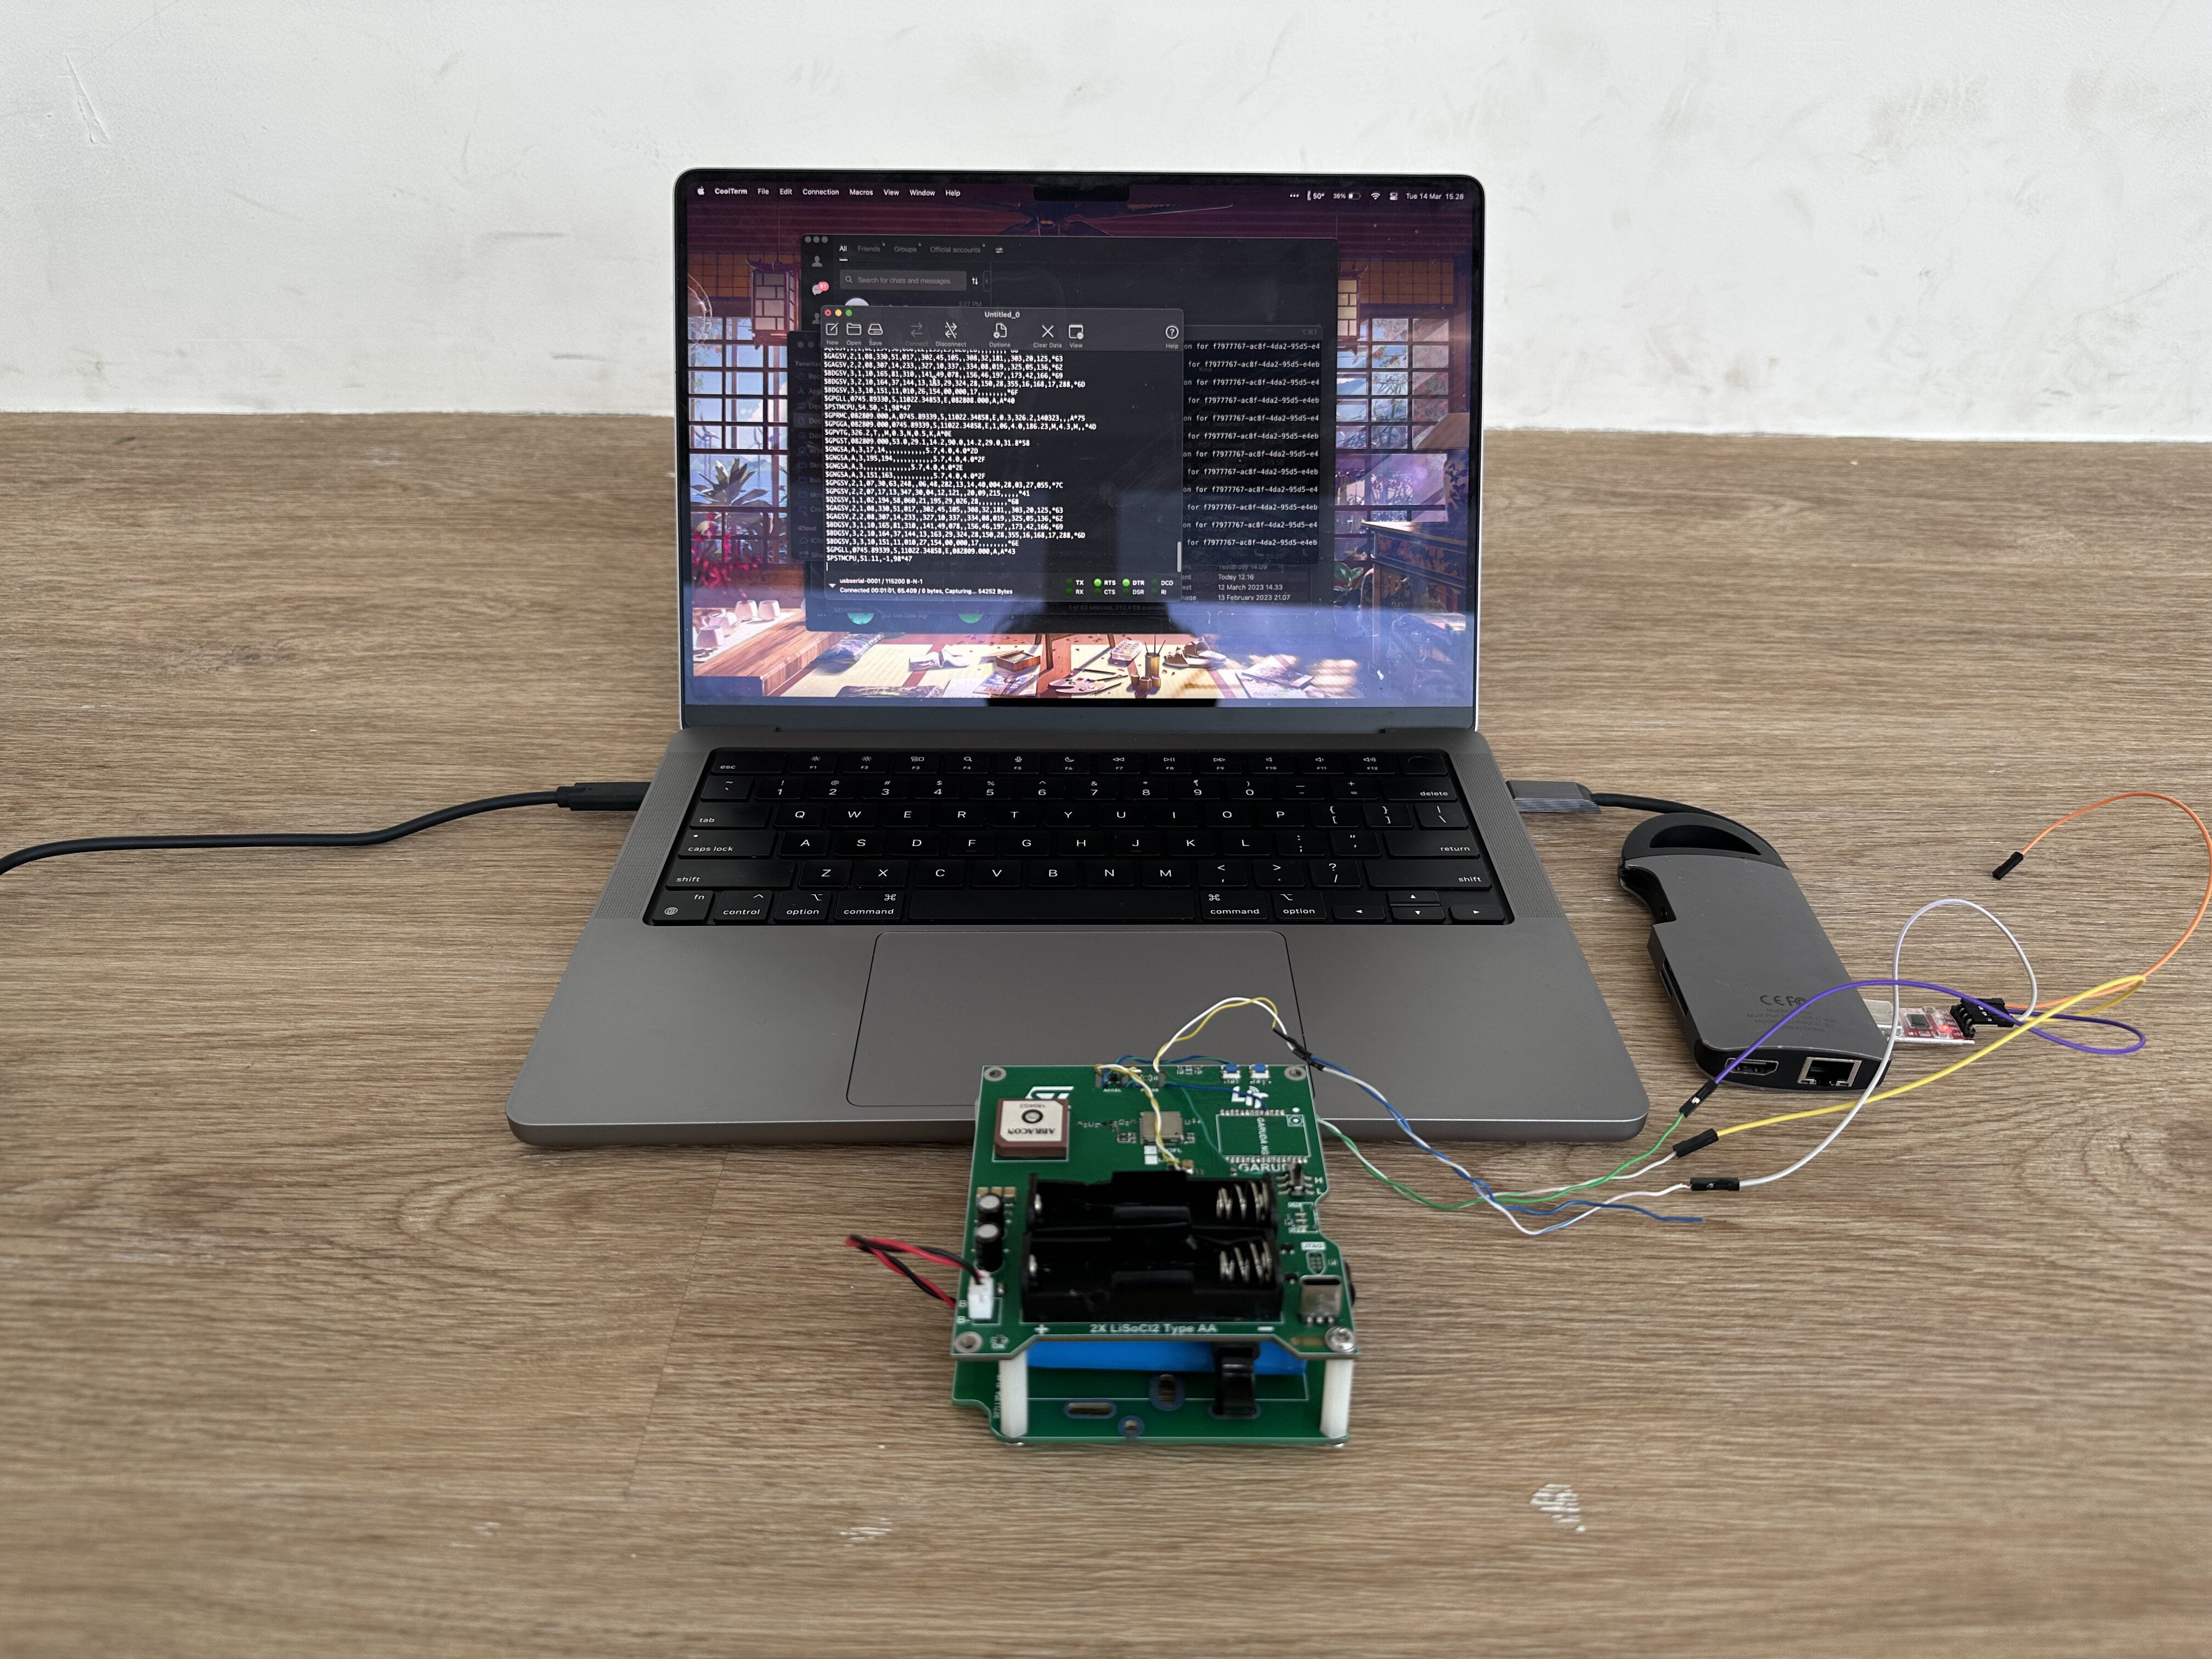
\includegraphics[width=8cm]{contents/chapter-4/2-skenario-indoor/keadaan.jpg}
	\caption{Pengujian Skenario Dalam Ruangan}
	\label{Fig: indoor-keadaan}
\end{figure}

Persebaran koordinat garis lintang dan garis bujur pada skenario dalam ruangan berada pada rentang -7,770949 hingga -7,770883 dan 110,377283 hingga 110,377315 seperti ditunjukan oleh Gambar \ref{Fig:indoor-distribution}. Modus dari kedua persebaran berada di titik -7.765039, 110.372458. Namun, seperti halnya dengan skenario sebelumnya, distribusi koordinat pada pengujian ini tidak terdistribusi secara normal, sehingga perlu dilakukan analisis pada nilai MAD-nya untuk mendapatkan pemahaman yang lebih baik mengenai data hasil pengujian.

\begin{figure}[H]
	\centering
	\begin{adjustbox}{width=\textwidth}
		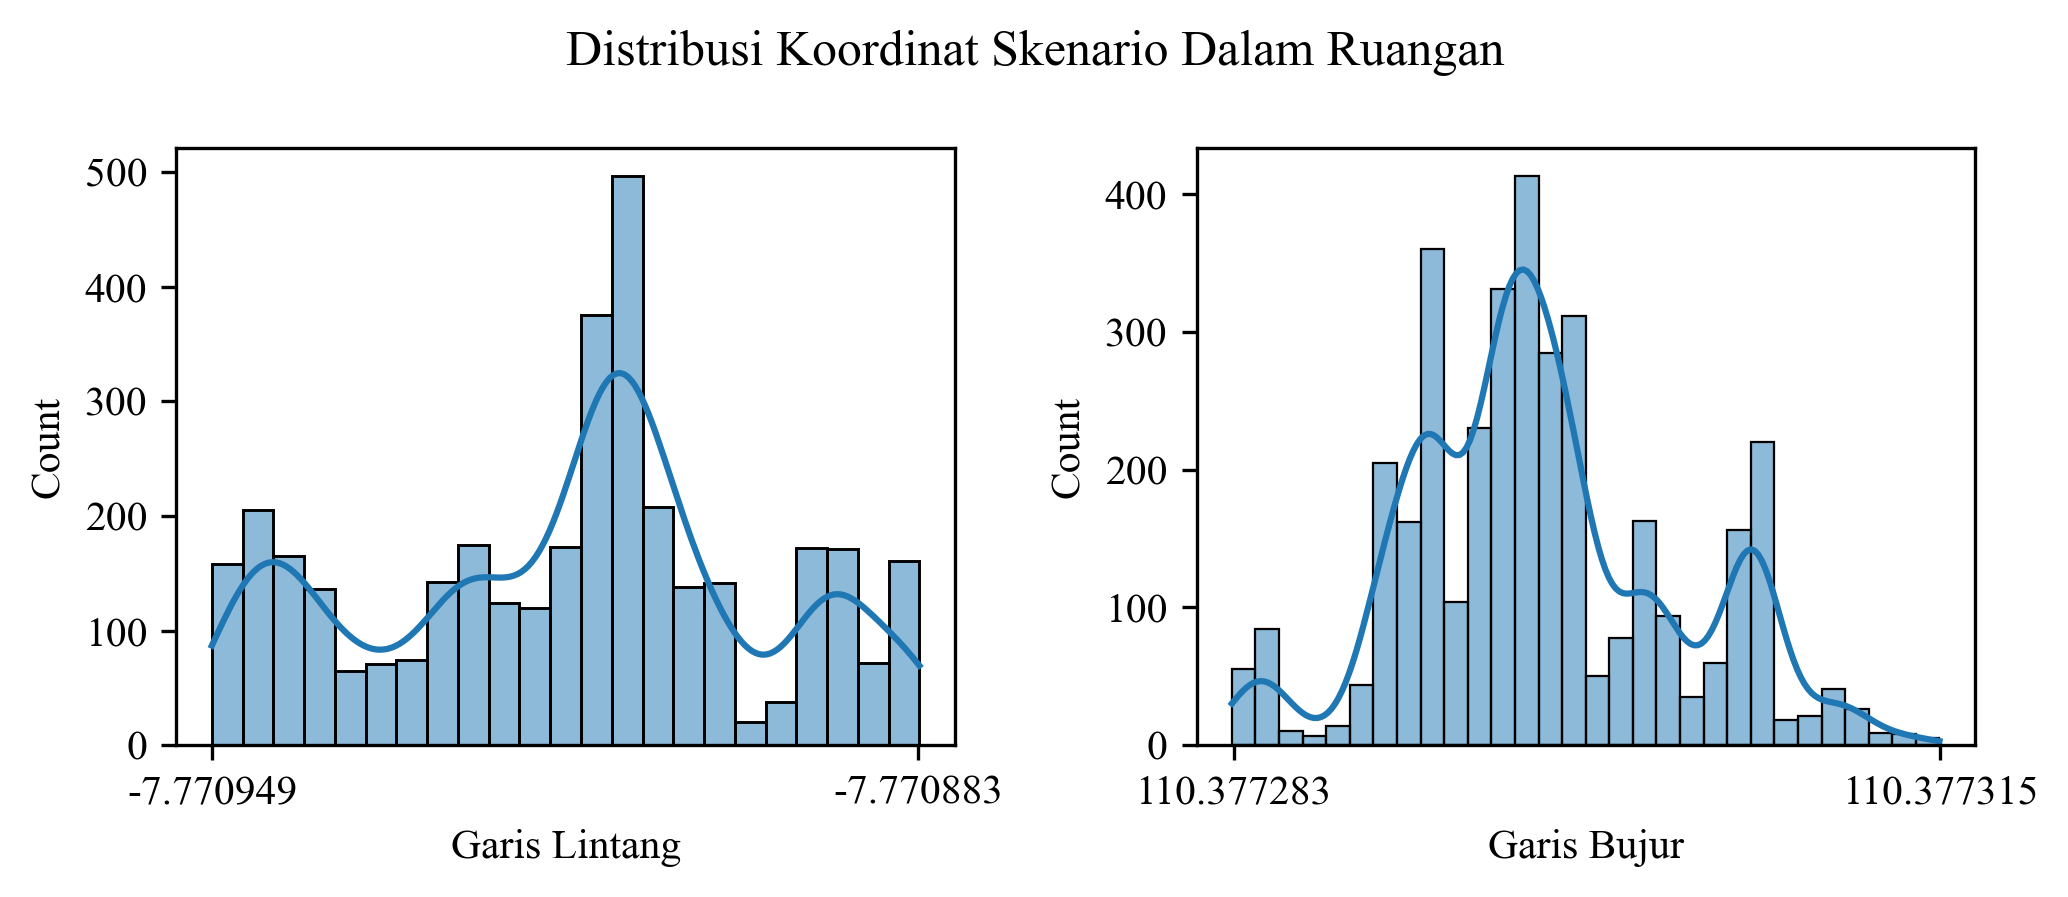
\includegraphics{contents/chapter-4/2-skenario-indoor/distribution.png}
	\end{adjustbox}
	\caption{Distribusi Data Koordinat Skenario Dalam Ruangan}
	\label{Fig:indoor-distribution}
\end{figure}

Tabel \ref{Tab: indoor-table} menunjukan hasil pengujian pada skenario dalam ruangan. Penurunan nilai DOP menunjukan bahwa hasil pengukuran modul Teseo-LIV3FL lebih akurat jika dibandingkan dengan skenario \textit{basement}. Selain itu, tingkat presisi pada skenario ini juga menjadi lebih baik, yaitu 7,39 meter pada koordinat garis lintangnya, 4,11 meter pada garis bujurnya, dan 8,46 meter secara keseluruhan.

\begin{table}[H]
	\caption{Hasil Pengujian Dalam Ruangan}
	\vspace{0.5em}
	\centering
	\begin{tabular}{ccccc}
		\hline
		& \textbf{Minima} & \textbf{Maxima} & \textbf{Rata-rata} & \textbf{Standar Deviasi}\\
		\hline 
		HDOP & 1,30 & 6,80 & 2,79 & 0,68\\
		PDOP & 2,00 & 8,40 & 3,73 & 0,74\\
		VDOP & 1,40 & 5,50 & 2,48 & 0,94\\
		Jumlah Satelit & 8 & 15 & 10,93 & 1,14\\
		\hline
		\textbf{MAD-x (m)} & & \multicolumn{2}{c}{\centering 12,14} & \\
		\hline
		\textbf{MAD-y (m)} & & \multicolumn{2}{c}{\centering 12,14} & \\
		\hline
		\textbf{MAD (m)} & & \multicolumn{2}{c}{\centering 8,46} & \\
		\hline
	\end{tabular}
	\label{Tab: indoor-table}
\end{table}

\begin{figure}[H]
	\centering
	\captionsetup{justification=centering}
	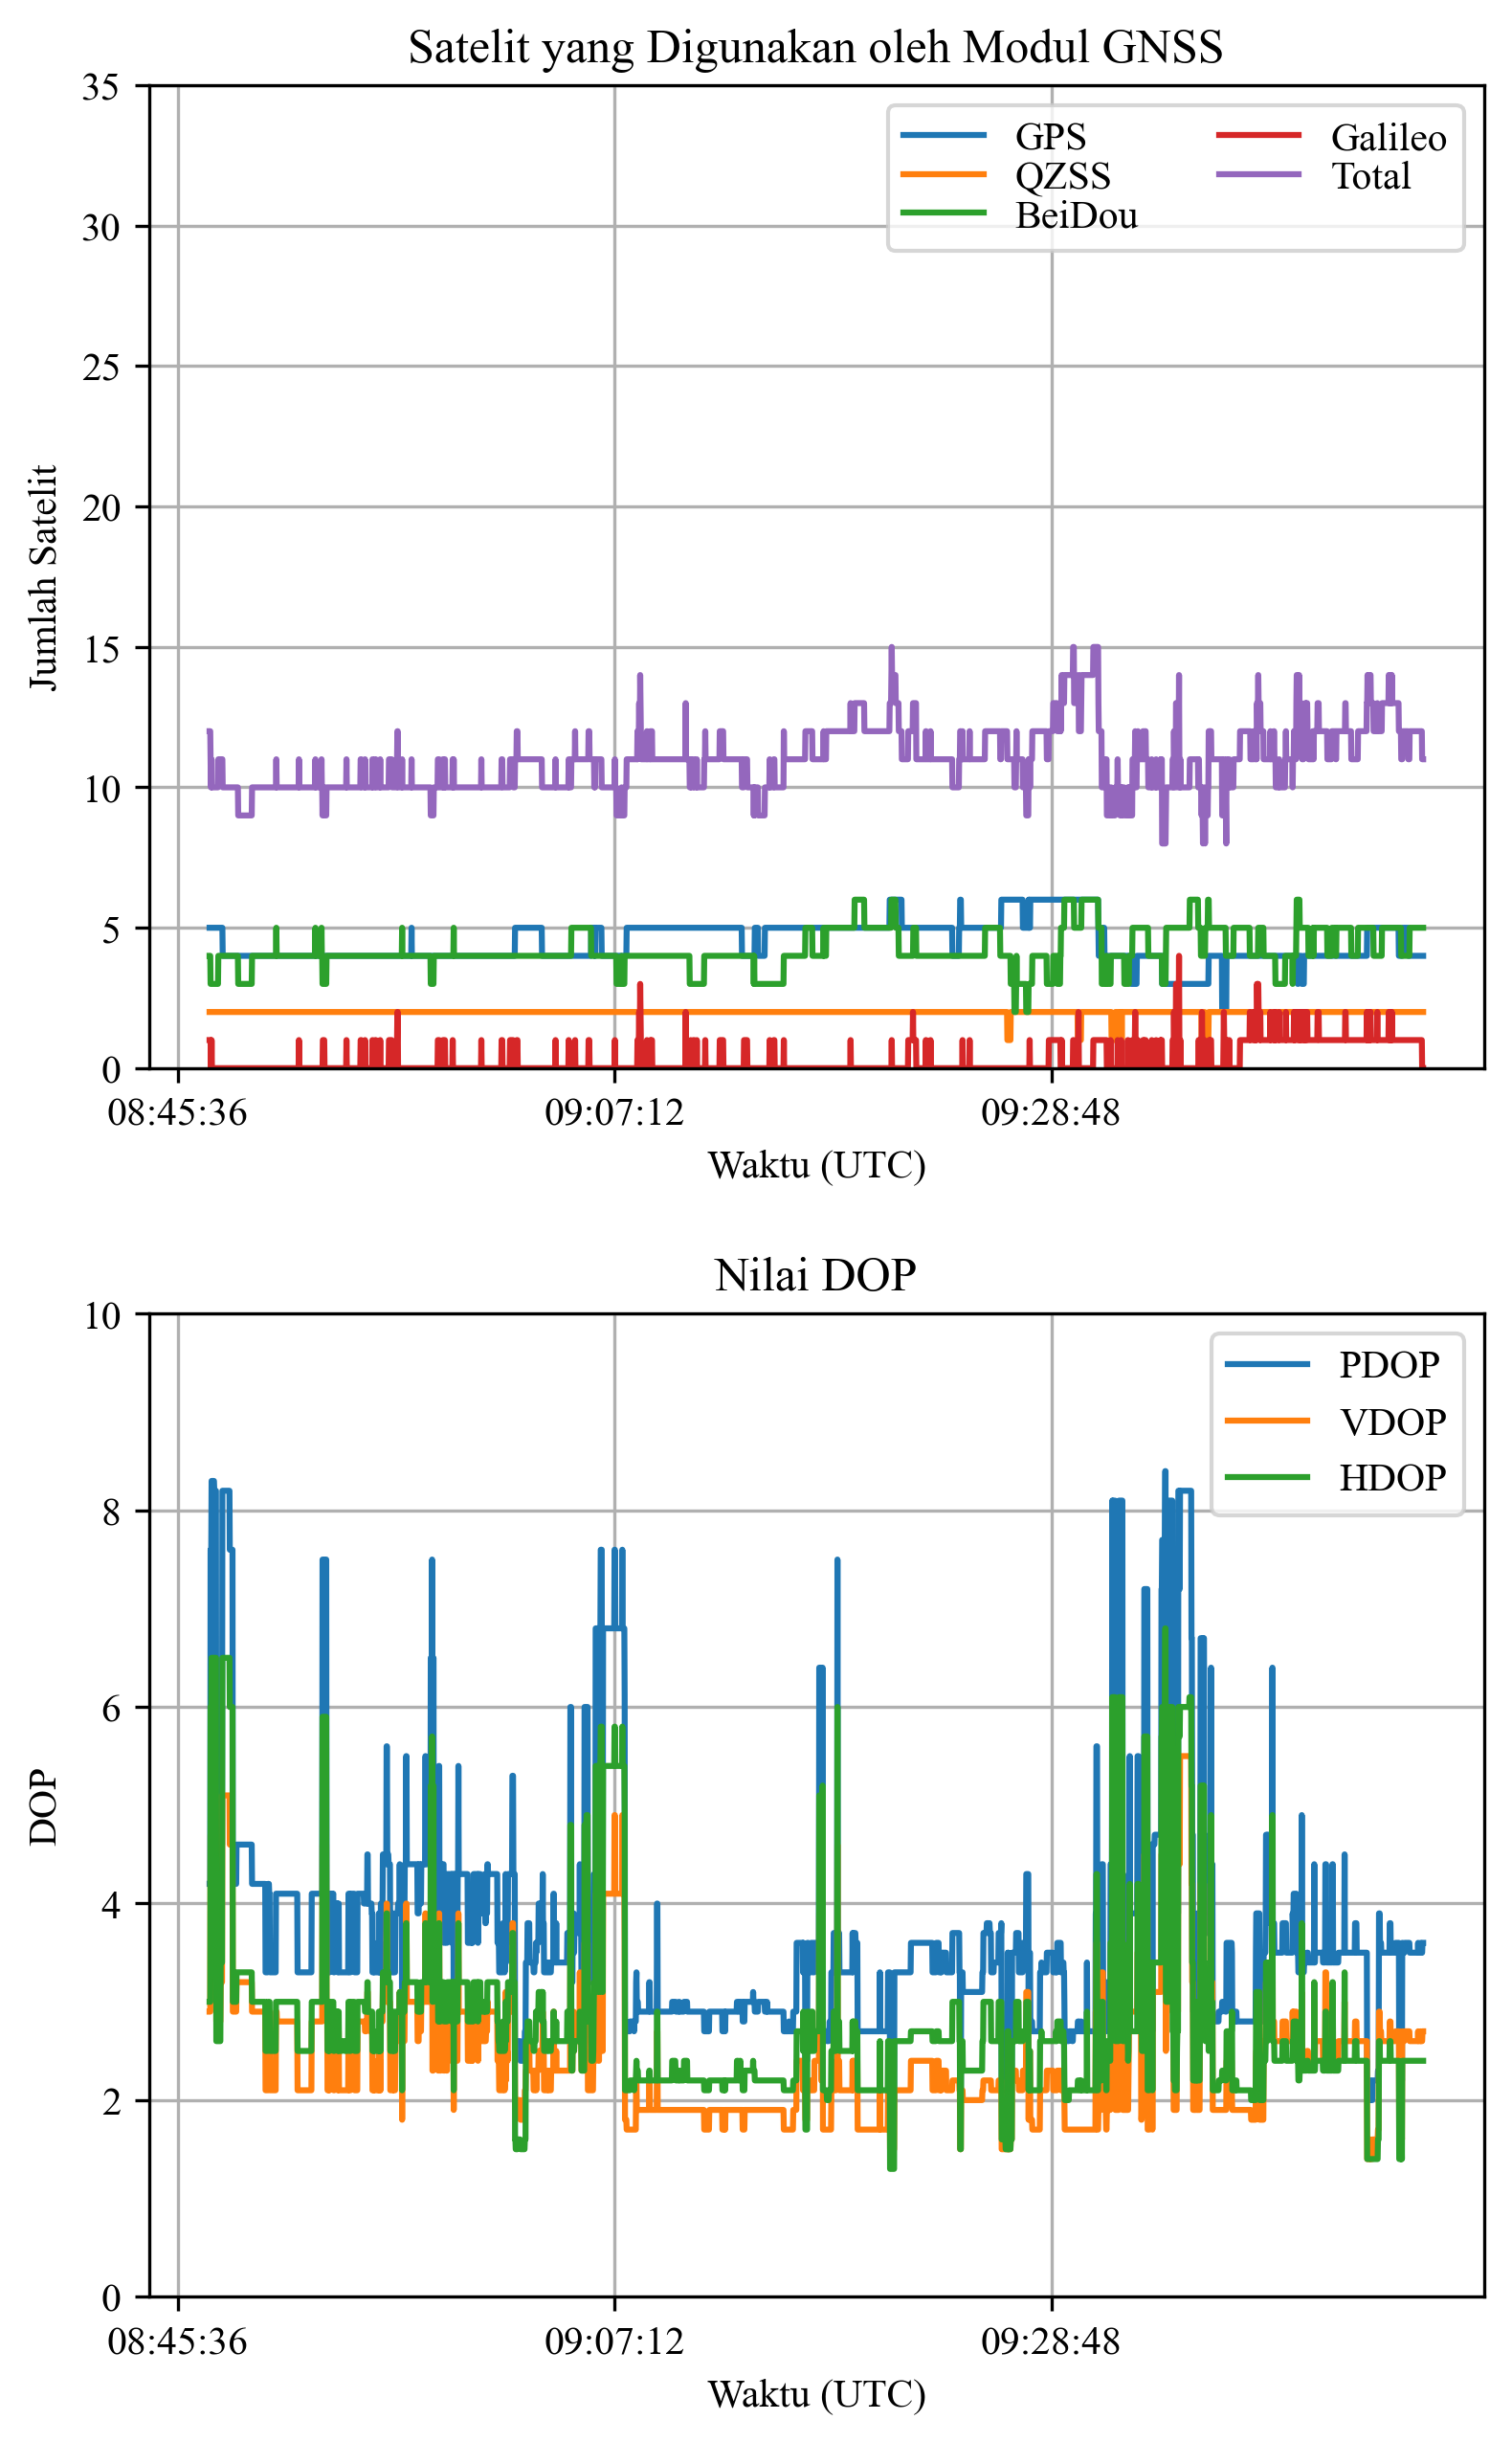
\includegraphics[width=12cm]{contents/chapter-4/2-skenario-indoor/sats_dop.png}
	\caption{DOP dan Visibilitas Satelit Pengujian Skenario Dalam Ruangan Tertutup}
	\label{Fig: indoor-sats_dop}
\end{figure}

Sama seperti pada pengujian skenario \textit{basement}, modul Teseo-LIV3FL juga dapat menerima isyarat dari keempat konstelasi yang telah diatur sebelumnya seperti ditunjukan pada Gambar \ref{Fig: indoor-sats_dop}. Dari hasil pengujian ini, terlihat bahwa konstelasi dengan jumlah satelit terbanyak adalah BeiDou dan GPS, yang dapat memberikan sinyal yang lebih kuat dan lebih akurat dalam mendukung navigasi satelit. Sementara itu, jumlah satelit pada konstelasi QZSS hampir selalu konstan pada dua buah satelit, sedangkan konstelasi Galileo dapat bervariasi antara nol hingga empat buah satelit tergantung pada kondisi lingkungan di sekitar pengujian. 

Terakhir, \textit{sky plot} pada Gambar \ref{Fig: indoor-sky_plot} menunjukan jika satelit pada skenario ini lebih tersebar jika dibandingkan dengan skenario sebelumnya. Hal ini juga sejalan dengan penurunan nilai PDOP seperti yang ditunjukan oleh Tabel \ref{Tab: indoor-table}.

\begin{figure}[H]
	\centering
	\captionsetup{justification=centering}
	\includegraphics[width=12cm]{contents/chapter-4/2-skenario-indoor/sky_plot.png}
	\caption{\textit{Sky Plot} Skenario Dalam Ruangan}
	\label{Fig: indoor-sky_plot}
\end{figure}

Tingkat kepresisian modul Teseo-LIV3FL yang diwakili oleh nila MAD adalah sebesar 8,46 meter atau 65,6\% lebih presisi dibandingkan pada skenario \textit{basement}. Rata-rata nilai HDOP pada pengujian ini adalah 2,79 yang menunjukan bahwa hasil pengukuran sudah baik dan tepat berada pada standar minimum pengukuran. Struktur beton yang lebih sedikit dapat membantu untuk meningkatkan performa GNSS terlihat pada semakin banyak satelit yang dapat digunakan dan penurunan pada nilai CEP dan ketiga nilai DOP.

\subsection{Skenario Ruangan Semi Terbuka}
Pengujian skenario ruangan semi terbuka dilakukan untuk mengevaluasi performa modul Teseo-LIV3FL di luar ruangan dengan adanya penghalang seperti pohon, atap, dan lain sebagainya. Titik pengujian berada di Selasar Grha Sabha Pramana, sebuah ruangan semi terbuka yang terdapat penghalang berupa tingkat dua Grha Sabha Pramana serta pepohonan yang berada di sekitar ruangan. Kondisi lingkungan yang ada pada pengujian ini jauh berbeda dengan pengujian dalam ruangan atau pengujian di \textit{basement}. Gambar \ref{Fig: semioutdoor-keadaan} menunjukan pengujian skenario ruangan semi terbuka.

\begin{figure}[H]
	\centering
	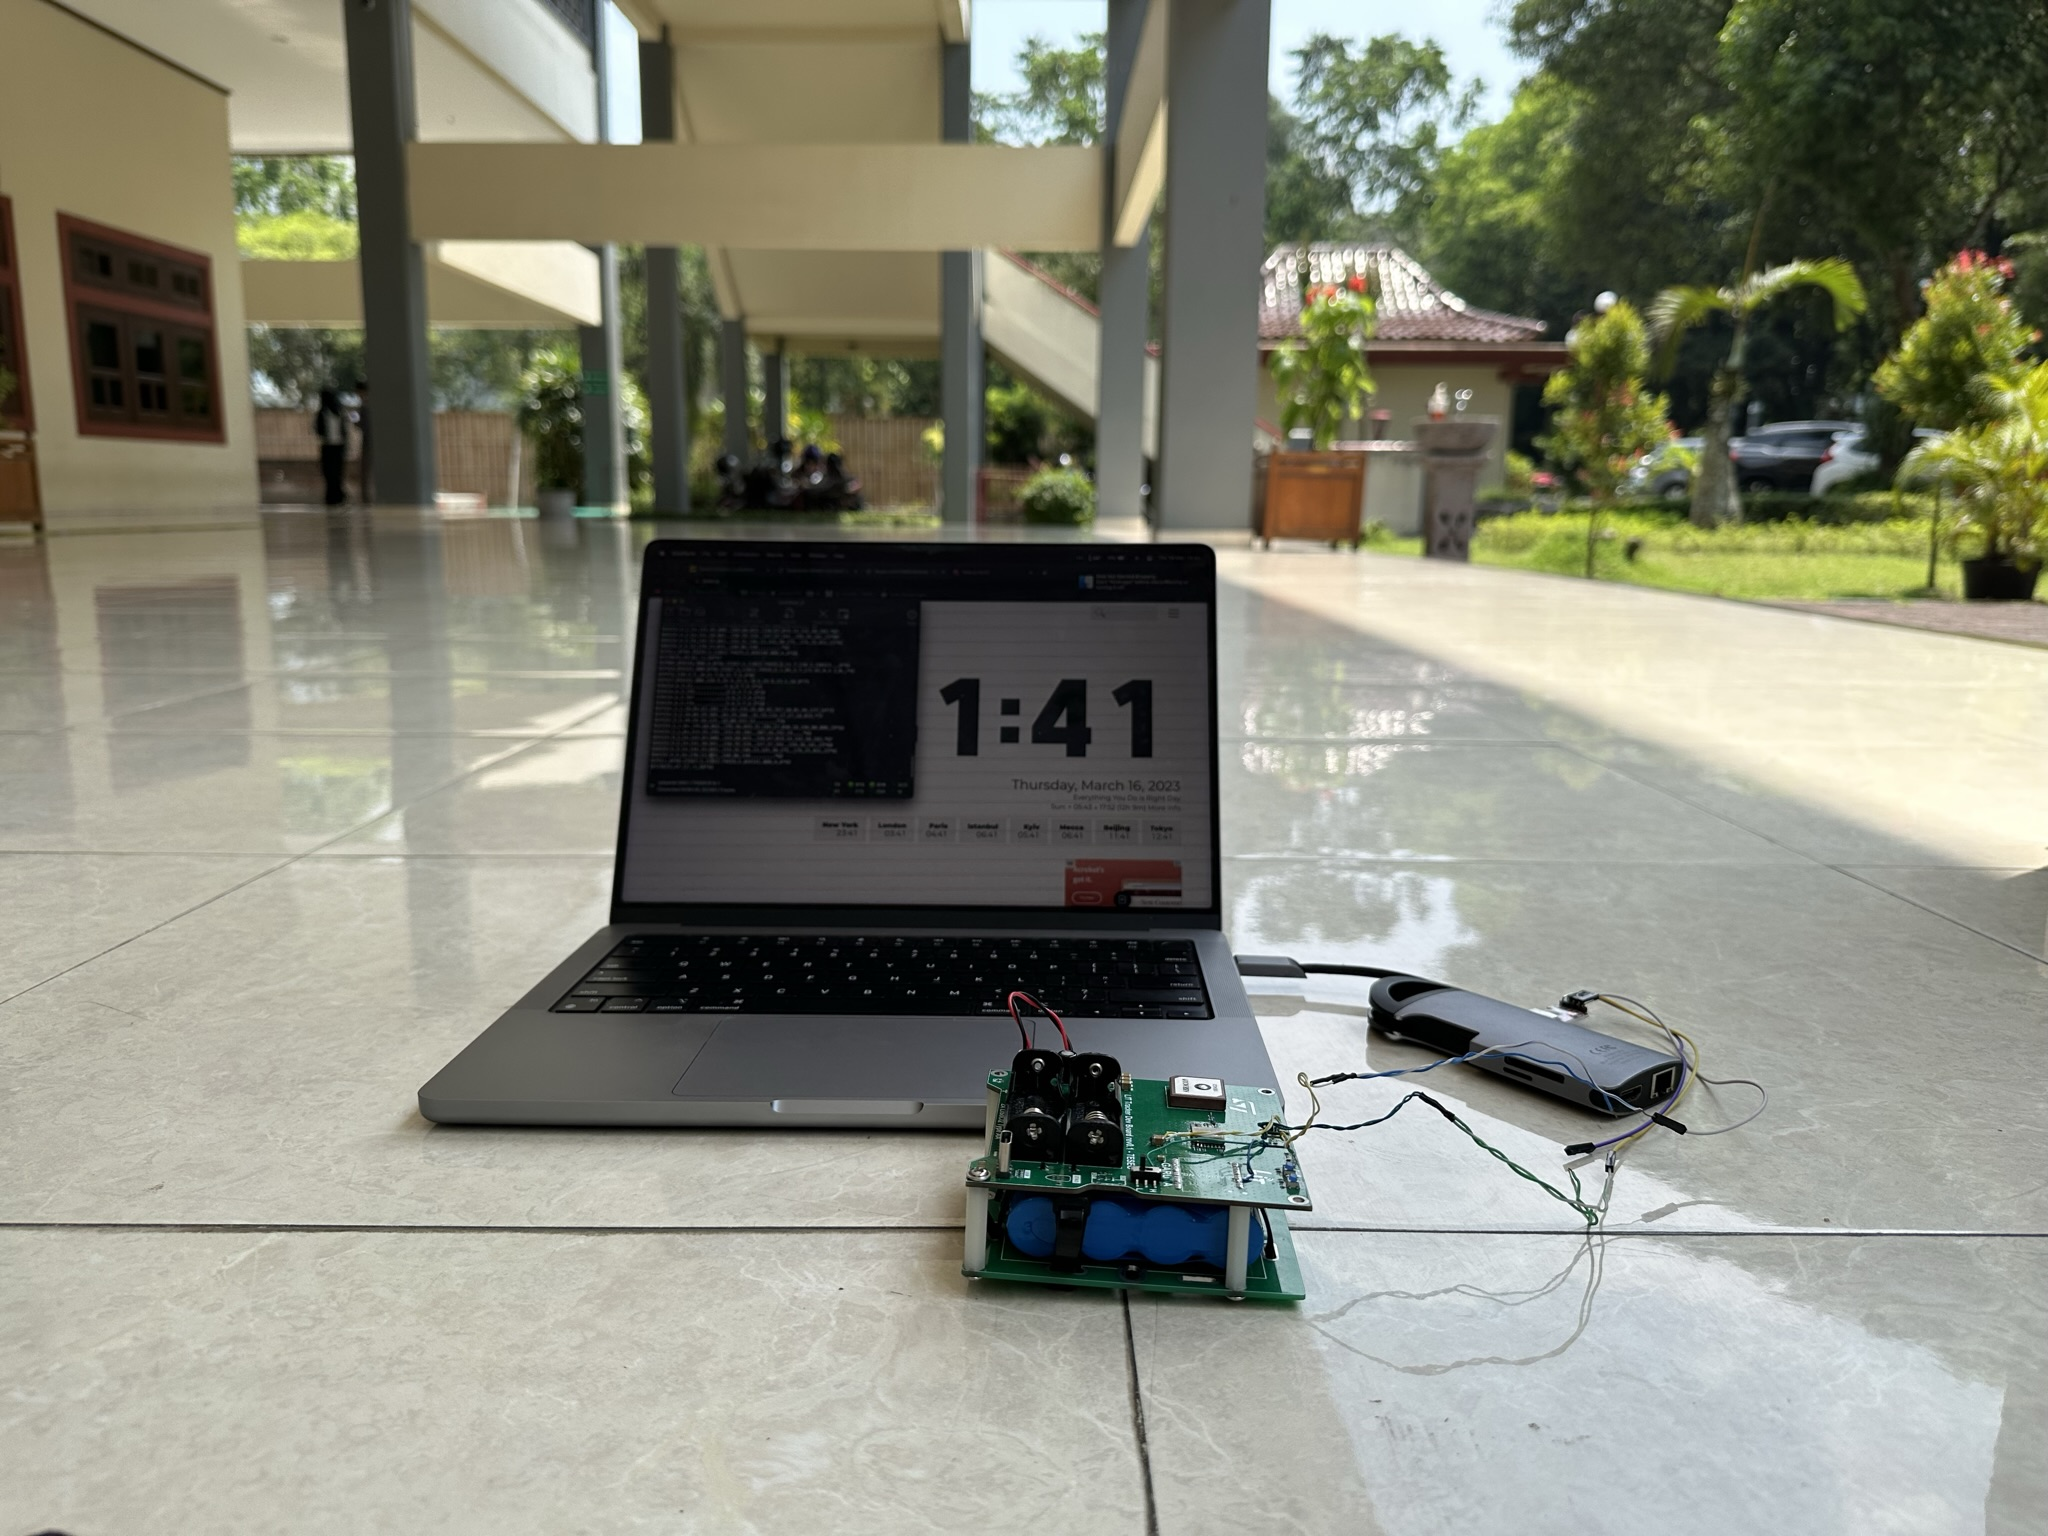
\includegraphics[width=10cm]{contents/chapter-4/3-skenario-semioutdoor/keadaan.jpeg}
	\caption{Pengujian Skenario Ruangan Semi Terbuka}
	\label{Fig: semioutdoor-keadaan}
\end{figure}

Sama seperti hasil pengujian pada dua skenario sebelumnya, data koordinat garis lintang dan garis bujur pada pengujian skenario ruang semi terbuka tidak terdistribusi normal seperti ditunjukan oleh \textit{kernel density estimator} Gambar \ref{Fig:semioutdoor-distribution}. Oleh karena itu, pada pengujian ini juga akan dilakukan analisis terhadap nilai MAD-nya. Nilai koordinat garis lintang pada pengujian ini berada pada rentang -7,769902 hingga -7,769962 dan 110,377433 hingga 110,377460 untuk koordinat garis bujurnya.

\begin{figure}[H]
	\centering
	\begin{adjustbox}{width=\textwidth}
		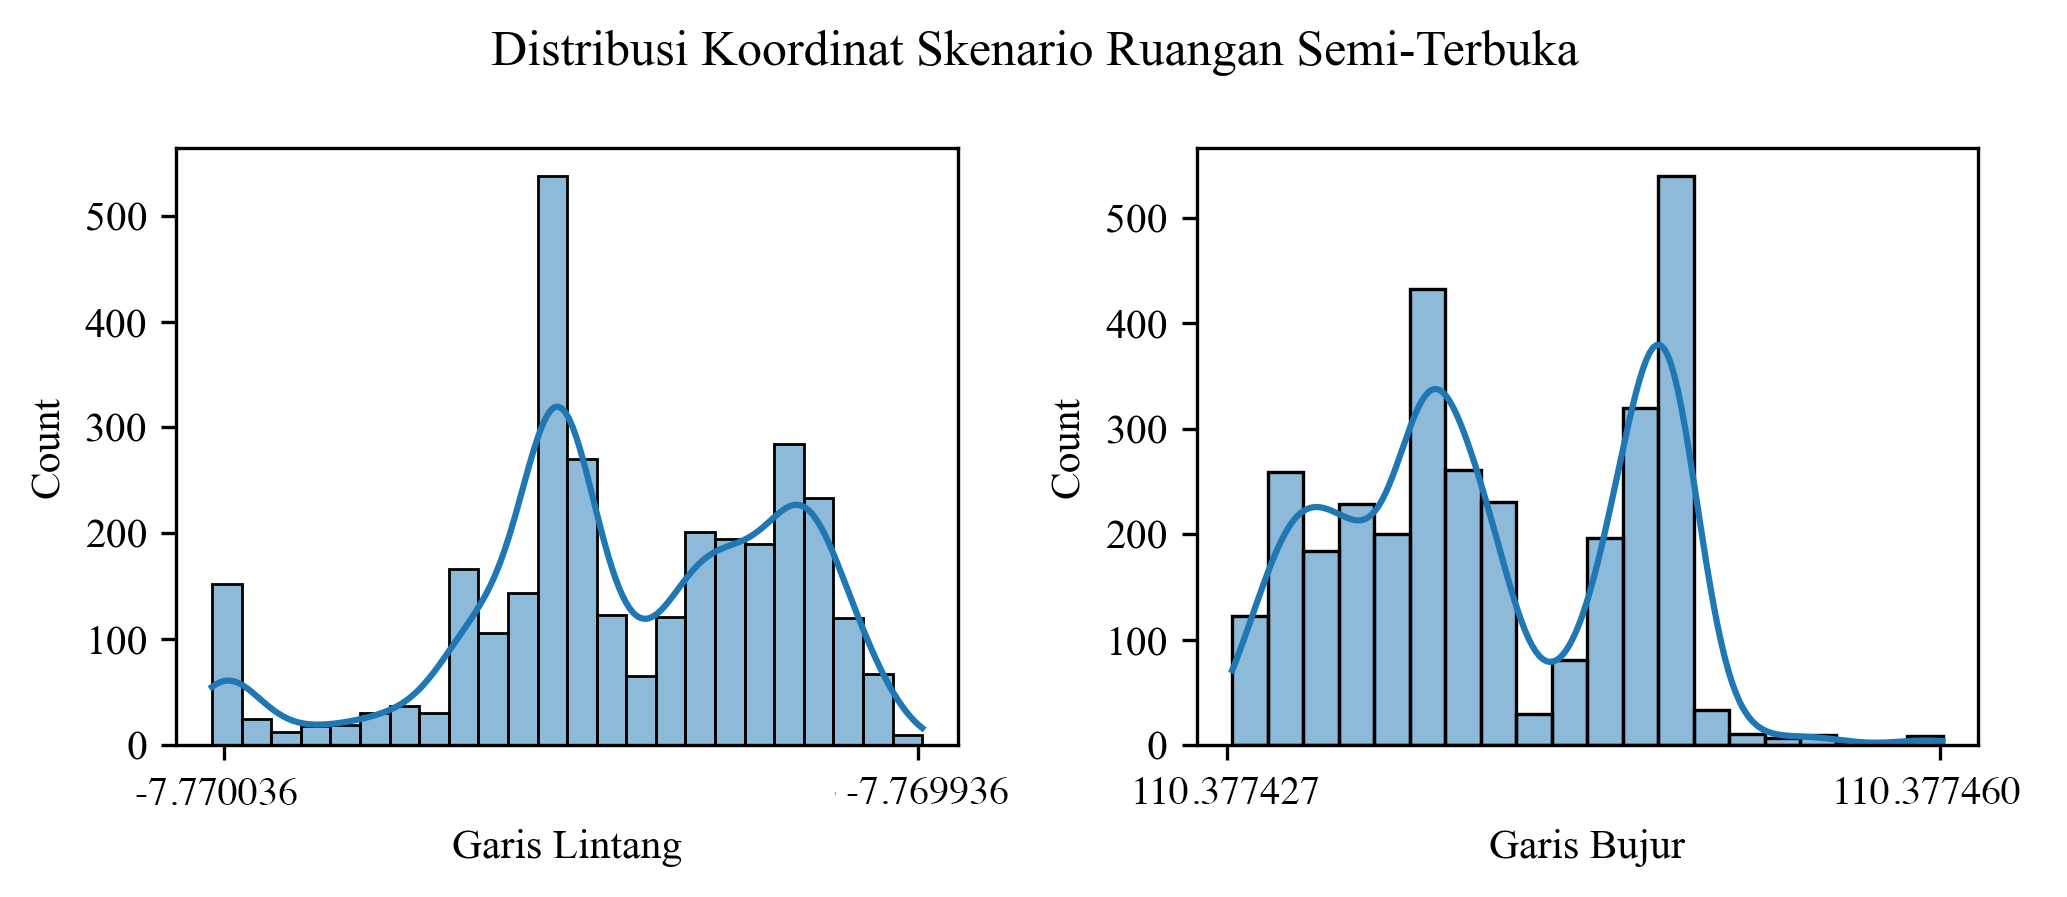
\includegraphics{contents/chapter-4/3-skenario-semioutdoor/distribution.png}
	\end{adjustbox}
	\caption{Distribusi Data Koordinat Skenario Ruangan Semi Terbuka}
	\label{Fig:semioutdoor-distribution}
\end{figure}

Pada hasil pengujian yang ditunjukan oleh Tabel \ref{Tab: outdoor-table}, ditemukan bahwa terjadi penurunan pada ketiga nilai DOP seiring dengan peningkatan jumlah satelit yang digunakan, yang menunjukkan bahwa akurasi dari modul Teseo-LIV3FL semakin meningkat. Selain itu, kepresisian dari modul ini juga mengalami peningkatan yang signifikan, dengan nilai 2,29 pada koordinat garis lintang, 2,02 pada koordinat garis bujur, dan 3,06 pada kepresisian keseluruhan.

\begin{table}[H]
	\caption{Hasil Pengujian di Ruangan Semi Terbuka}
	\vspace{0.5em}
	\centering
	\begin{tabular}{ccccc}
		\hline
		& \textbf{Minima} & \textbf{Maxima} & \textbf{Rata-rata} & \textbf{Standar Deviasi}\\
		\hline 
		HDOP & 0,80 & 1,40 & 0,91 & 0,12\\
		PDOP & 1,50	& 3,00 & 1,75 & 0,25\\
		VDOP & 1,20	& 2,70 & 1,49 & 0,23\\
		Jumlah Satelit & 10 & 18 & 14,32 & 1,41\\
		\hline
		\textbf{MAD-x (m)} & & \multicolumn{2}{c}{\centering 2,29} & \\
		\hline
		\textbf{MAD-y (m)} & & \multicolumn{2}{c}{\centering 2,02} & \\
		\hline
		\textbf{MAD (m)} & & \multicolumn{2}{c}{\centering 3,06} & \\
		\hline
	\end{tabular}
	\label{Tab: semioutdoor-table}
\end{table}

Pada pengujian ini, urutan konstelasi dengan jumlah satelit paling banyak hingga paling sedikit adalah GPS, BeiDou, QZSS, dan BeiDou. Rata-rata jumlah satelit yang digunakan adalah 14,32 dengan jumlah terbanyak 18 buah seperti ditunjukan pada Tabel \ref{Tab: semioutdoor-table}. Visibilitas satelit pada skenario ruangan semi terbuka lebih baik jika dibandingkan dengan dua skenario sebelumnya. Gambar \ref{Fig: semioutdoor-sats_dop} menunjukan bahwa konstelasi dengan visibilitas satelit paling banyak adalah konstelasi BeiDou dan GPS.

\begin{figure}[H]
	\centering
	\captionsetup{justification=centering}
	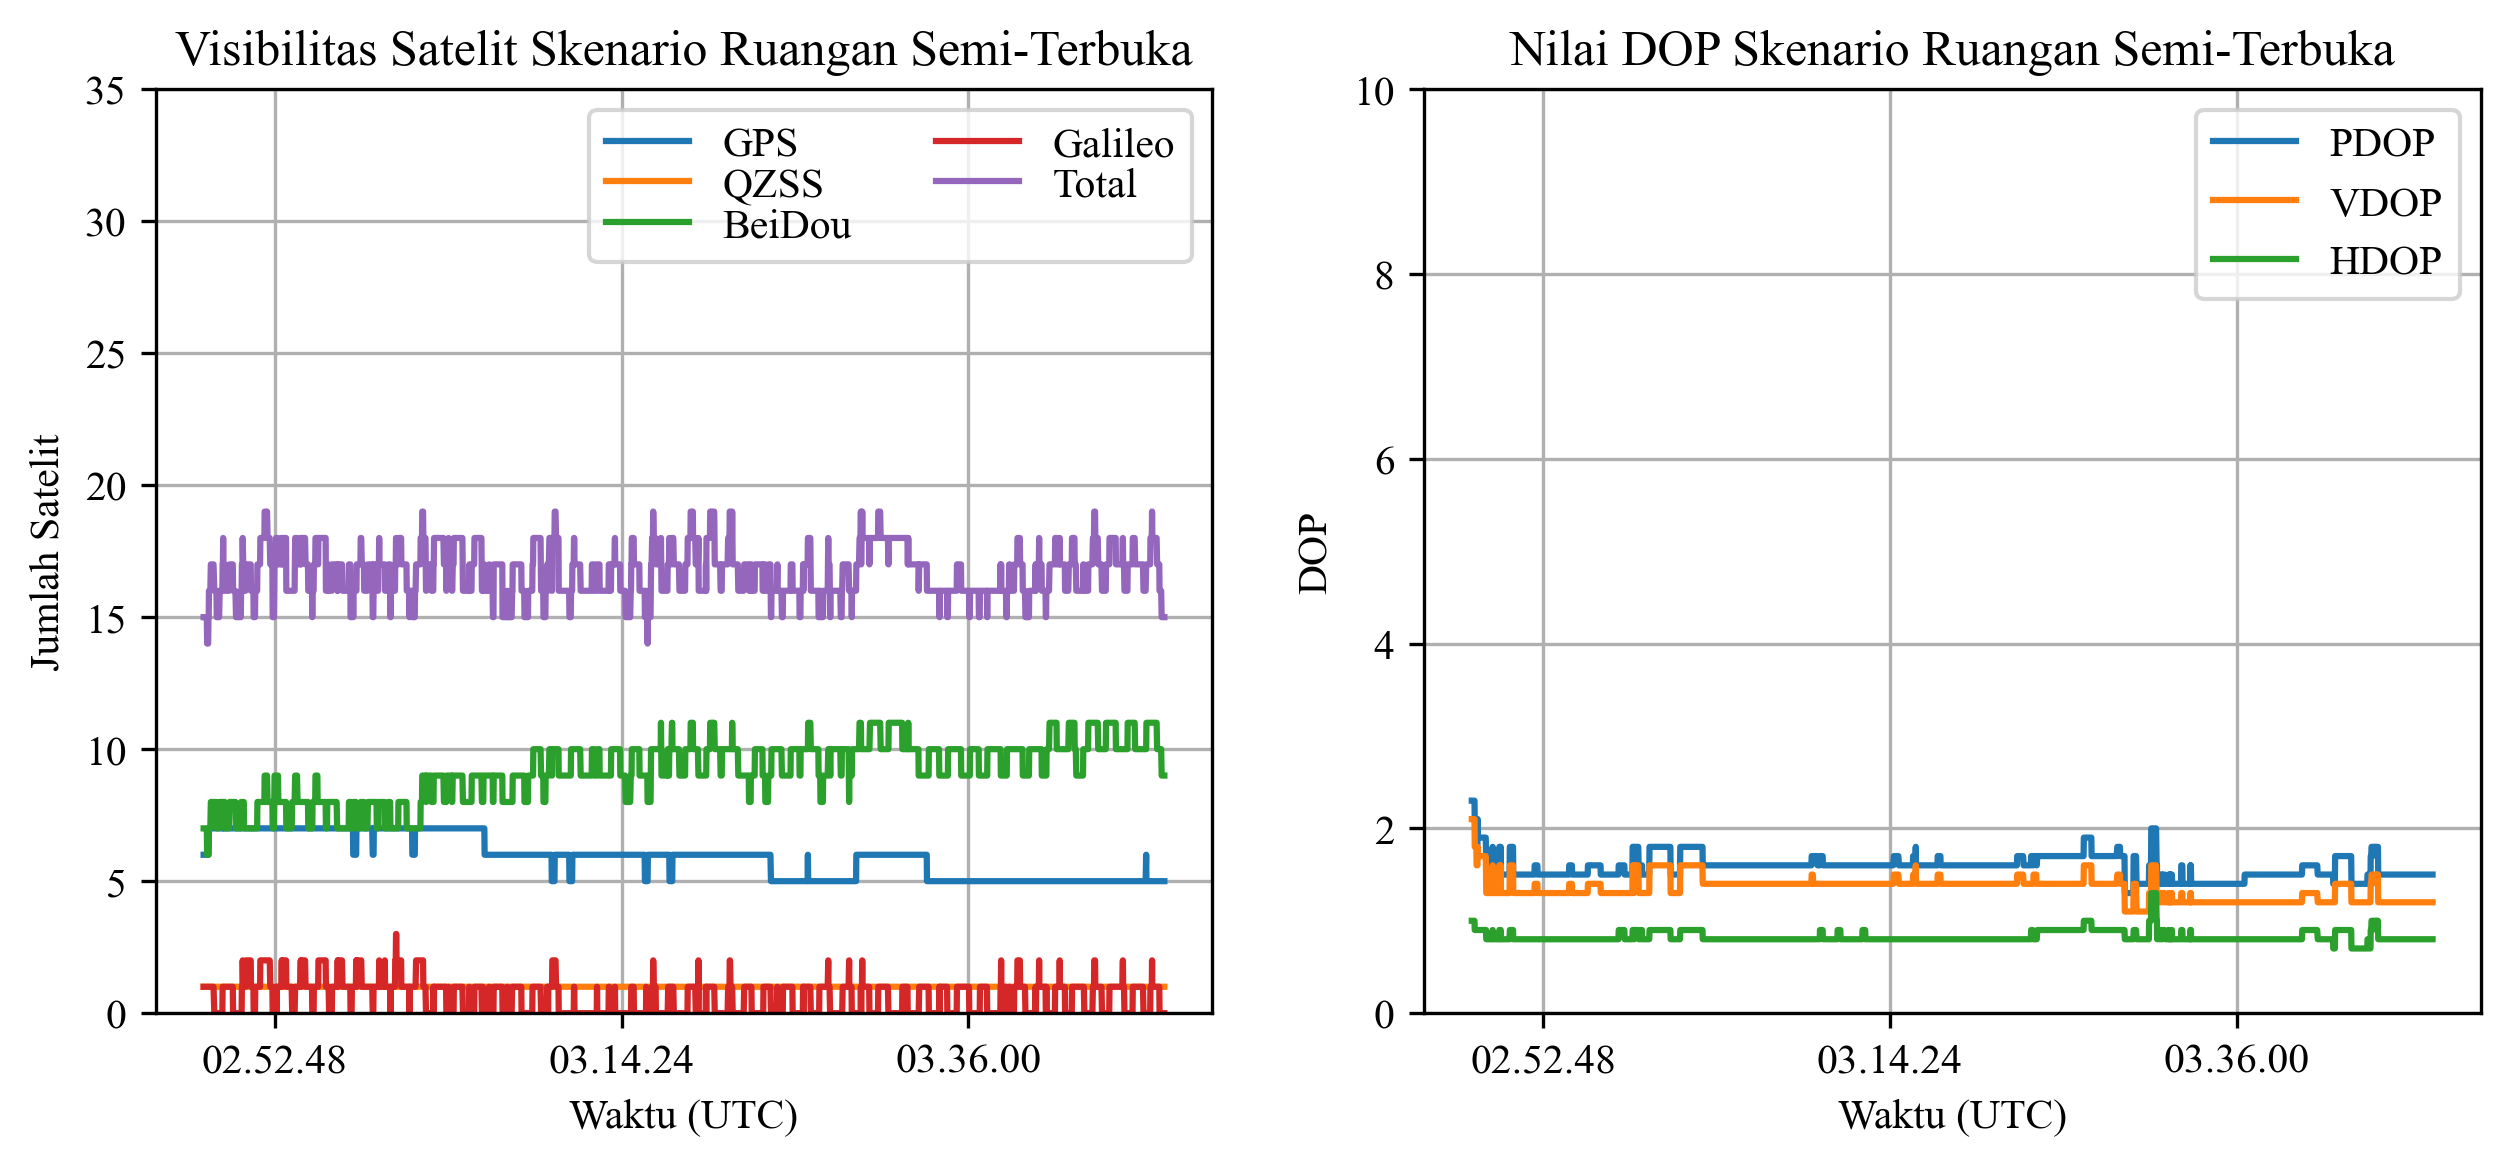
\includegraphics[width=11.5cm]{contents/chapter-4/3-skenario-semioutdoor/sats_dop.png}
	\caption{DOP dan Visibilitas Satelit Pengujian Skenario Ruangan Semi Terbuka}
	\label{Fig: semioutdoor-sats_dop}
\end{figure}

Jika ditinjau dari nilai DOP, ketiga nilai DOP juga mengalami penurunan secara signifikan. Penurunan nilai HDOP menunjukan terdapat peningkatan akurasi pada hasil pembacaan di bidang horizontal, sedangkan penurunan nilai VDOP menunjukan peningkatan akurasi pada pembacaan ketinggian. Gambar \ref{Fig: semioutdoor-sky_plot} menunjukan persebaran satelit di langit sudah mencakup seluruh kuadran lingkaran. Hal tersebut juga didukung oleh nilai PDOP yang lebih rendah.

\begin{figure}[H]
	\centering
	\captionsetup{justification=centering}
	\includegraphics[width=12cm]{contents/chapter-4/3-skenario-semioutdoor/sky_plot.png}
	\caption{\textit{Sky Plot} Skenario Ruangan Semi Terbuka}
	\label{Fig: semioutdoor-sky_plot}
\end{figure}

Berdasarkan hasil yang didapat, pada pengujian skenario ini dapat dilihat bahwa penempatan modul Teseo-LIV3FL pada lingkungan dengan penghalang yang lebih sedikit dapat meningkatkan tingkat akurasinya. Rata-rata nilai PDOP dan VDOP sudah berada dalam rentang sangat baik dan HDOP berada dalam rentang ideal yang artinya sudah dapat digunakan dalam aplikasi yang sensitif terhadap ketelitian. Selain itu, hasil pengukuran modul pada skenario ini lebih presisi 63,8\% lebih presisi jika dibandingkan dengan skenario dalam ruangan.

\subsection{Skenario Ruangan Terbuka}
Pengujian skenario ruangan terbuka bertujuan untuk meninjau performa modul Teseo-LIV3FL di ruangan terbuka. Titik pengujian berada di Lapangan Pancasila Universitas Gadjah Mada dengan kondisi langit cerah. Pemilihan lokasi Lapangan Pancasila bertujuan untuk meminimalisasi penghalang seperti gedung dan pepohonan. Gambar \ref{Fig: outdoor-keadaan} menunjukan pengujian skenasio ruangan terbuka. Berdasarkan penelitian \cite{Lu2018}, lingkungan dengan penghalang paling sedikit seperti skenario ruangan terbuka dapat meningkatkan ketelitian dan kepresisian dari modul GNSS.

\begin{figure}[H]
	\centering
	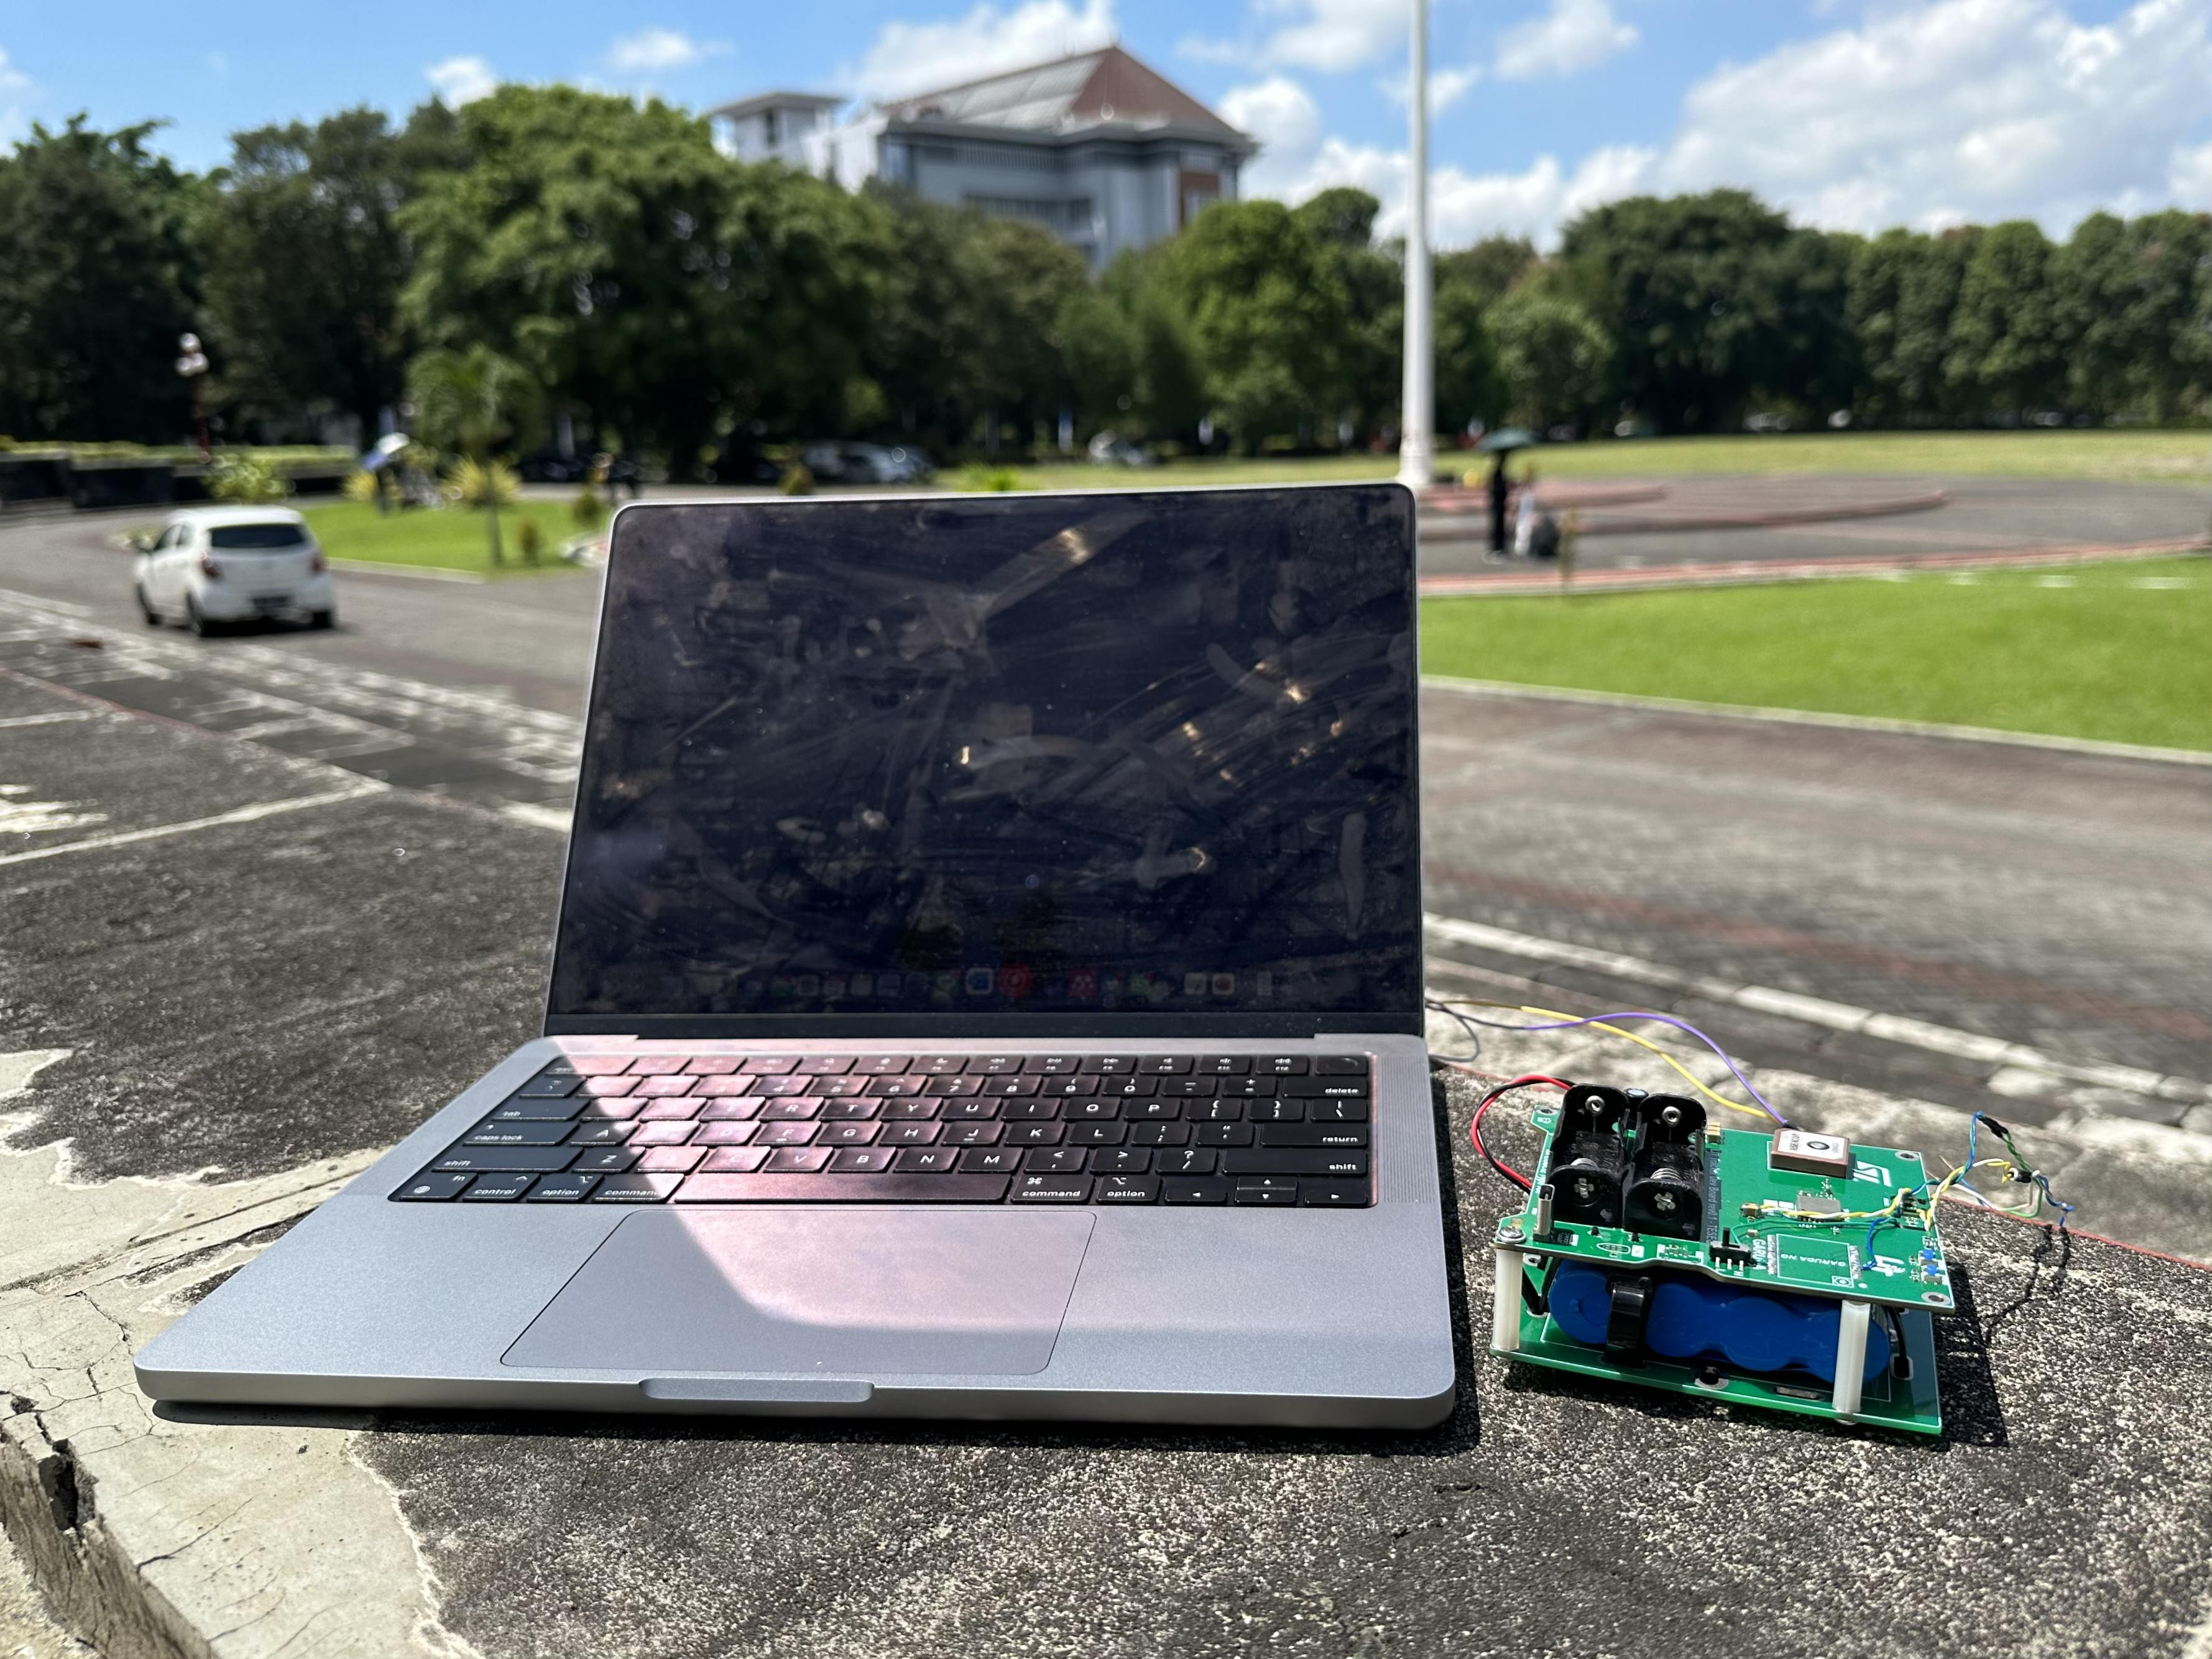
\includegraphics[width=10cm]{contents/chapter-4/4-skenario-outdoor/keadaan.jpg}
	\caption{Pengujian Skenario Ruang Terbuka}
	\label{Fig: outdoor-keadaan}
\end{figure}

Distribusi koordinat hasil pengujian luar ruangan ditunjukan oleh Gambar \ref{Fig:outdoor-distribution}. Koordinat garis lintang berada pada rentang -7,770949 hingga -7,770883, sedangkan koordinat garis bujur berada pada rentang 110,377283 hingga 110,377315. Sama seperti tiga pengujian sebelumnya, koordinat pada hasil pengujian ruang terbuka tidak terdistribusi normal. Karena data koordinat tidak terdistribusi normal maka akan dilakukan analisis terhadap nilai MAD-nya juga.

\begin{figure}[H]
	\centering
	\begin{adjustbox}{width=\textwidth}
		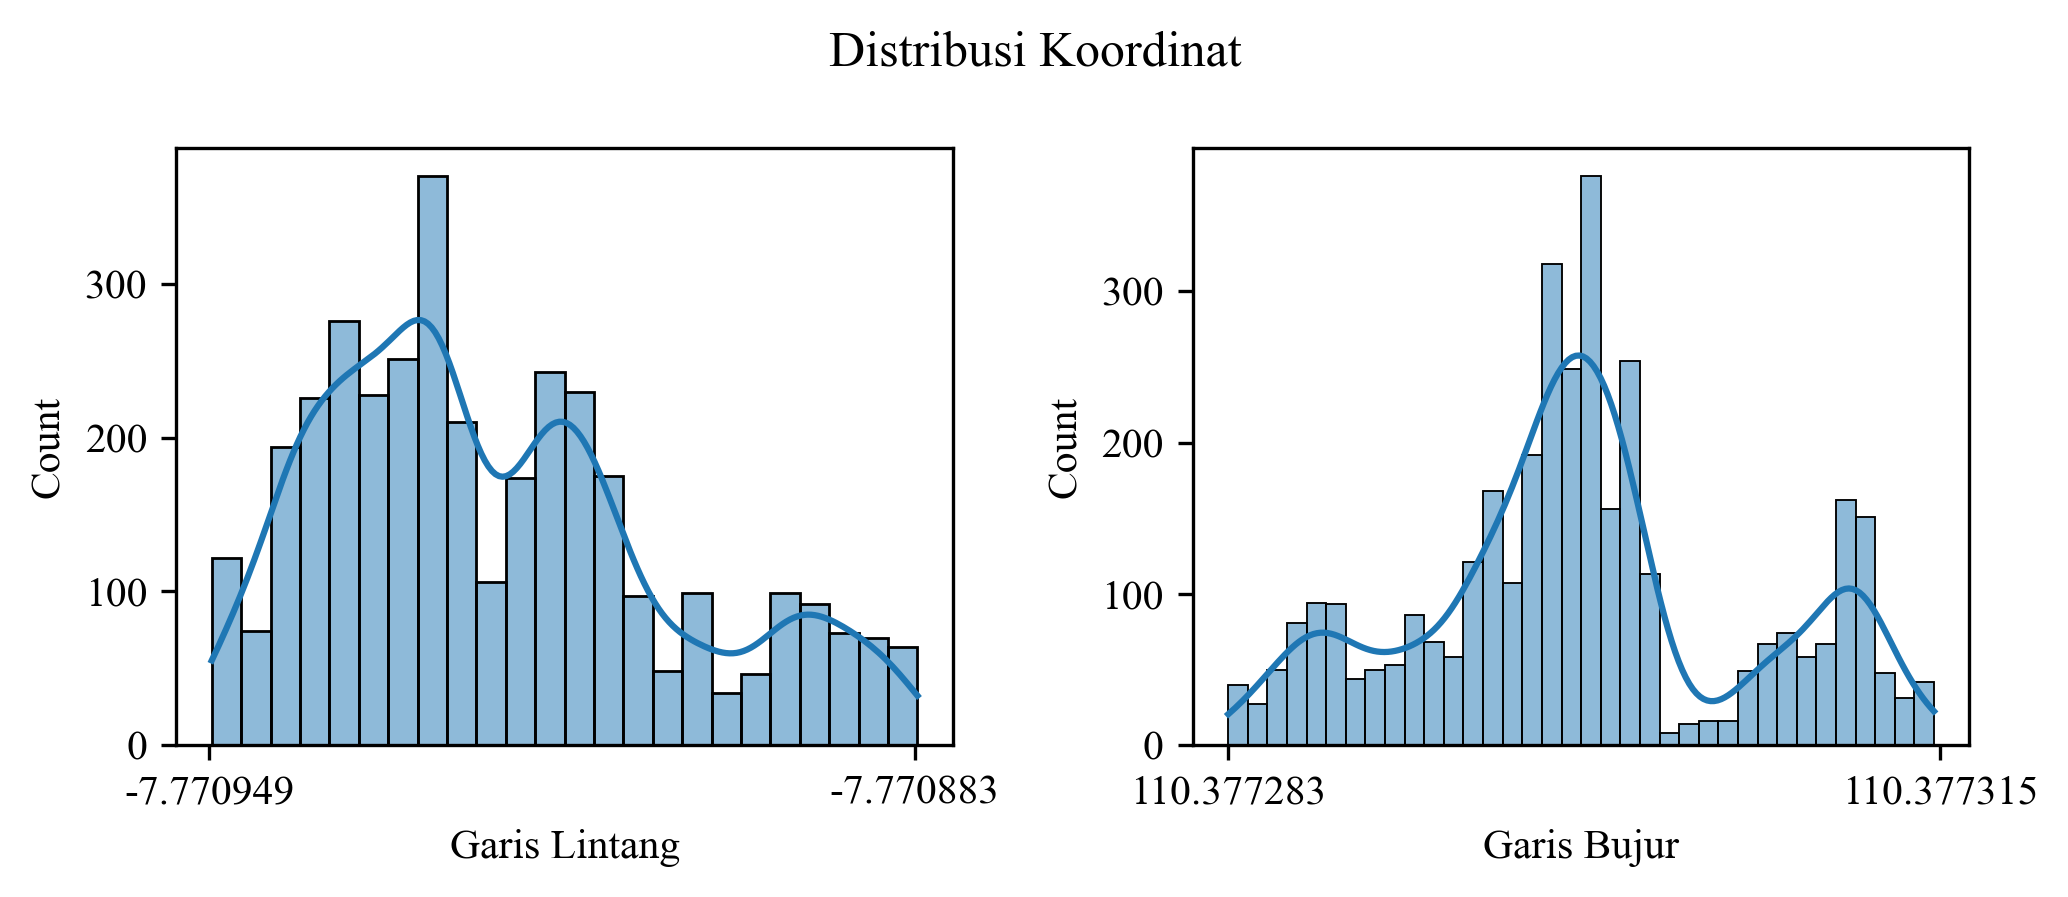
\includegraphics{contents/chapter-4/4-skenario-outdoor/distribution.png}
	\end{adjustbox}
	\caption{Distribusi Data Koordinat Skenario Ruang Terbuka}
	\label{Fig:outdoor-distribution}
\end{figure}

Tabel \ref{Tab: outdoor-table} menunjukan bahwa pada skenario ruang terbuka memberikan hasil akurasi yang lebih tinggi. Rata-rata nilai DOP yang didapat berada pada rentang sangat baik s.d. ideal. Rata-rata nilai PDOP yang didapat adalah sebesar 1,12 dengan PDOP terkecil adalah 0,90 dan terbesarnya 1,60. Nilai PDOP yang kecil didukung oleh persebaran satelit di langit yang lebih banyak mencakup bagian lingkaran pada Gambar \ref{Fig: outdoor-skyplot}. Tingkat kepresisian pada skenario ini ditunjukan oleh nilai MAD-nya, yaitu 0,94 meter untuk koordinat garis lingtang, 0,76 meter pada garis bujur, dan 1,21 meter untuk keseluruhannya.

\begin{table}[H]
	\caption{Hasil Pengujian Ruangan Terbuka}
	\vspace{0.5em}
	\centering
	\begin{tabular}{ccccc}
		\hline
		& \textbf{Minima} & \textbf{Maxima} & \textbf{Rata-rata} & \textbf{Standar Deviasi}\\
		\hline 
		HDOP & 0,60 & 0,80 & 0,65 & 0,06 \\
		PDOP & 0,90 & 1,60 & 1,12 & 0,15 \\
		VDOP & 1,10	& 1,80 & 1,30 & 0,15 \\
		Jumlah Satelit & 17	& 25 & 21,14 & 1,37 \\
		\hline
		\textbf{MAD-x (m)} & & \multicolumn{2}{c}{\centering 0,94} & \\
		\hline
		\textbf{MAD-y (m)} & & \multicolumn{2}{c}{\centering 0,76} & \\
		\hline
		\textbf{MAD (m)} & & \multicolumn{2}{c}{\centering 1,21} & \\
		\hline
	\end{tabular}
	\label{Tab: outdoor-table}
\end{table}

\begin{figure}[H]
	\centering
	\includegraphics[width=12cm]{contents/chapter-4/4-skenario-outdoor/sky_plot.png}
	\caption{\textit{Sky Plot} Pengujian Ruang Terbuka}
	\label{Fig: outdoor-skyplot}
\end{figure}

Gambar \ref{Fig: outdoor-dop_sats} menunjukan tren ketiga nilai DOP dan visibilitas satelit selama satu jam. Visibilitas satelit terkecil adalah tujuh belas satelit dan paling banyak adalah dua puluh lima satelit. Konstelasi GPS dan BeiDou masih menjadi konstelasi paling dominan, diikuti oleh konstelasi QZSS dengan visibilitas satelit stabil di antara dua sampai dengan lima satelit. Sementara itu, visibilitas satelit pada konstelasi Galileo bervariasi antara nol hingga dua satelit saja. Terdapat sedikit lonjakan pada nilai DOP, tetapi lonjakan tersebut tidak terlalu signifikan karena masih berada dalam kategori sangat baik.

\begin{figure}[H]
	\centering
	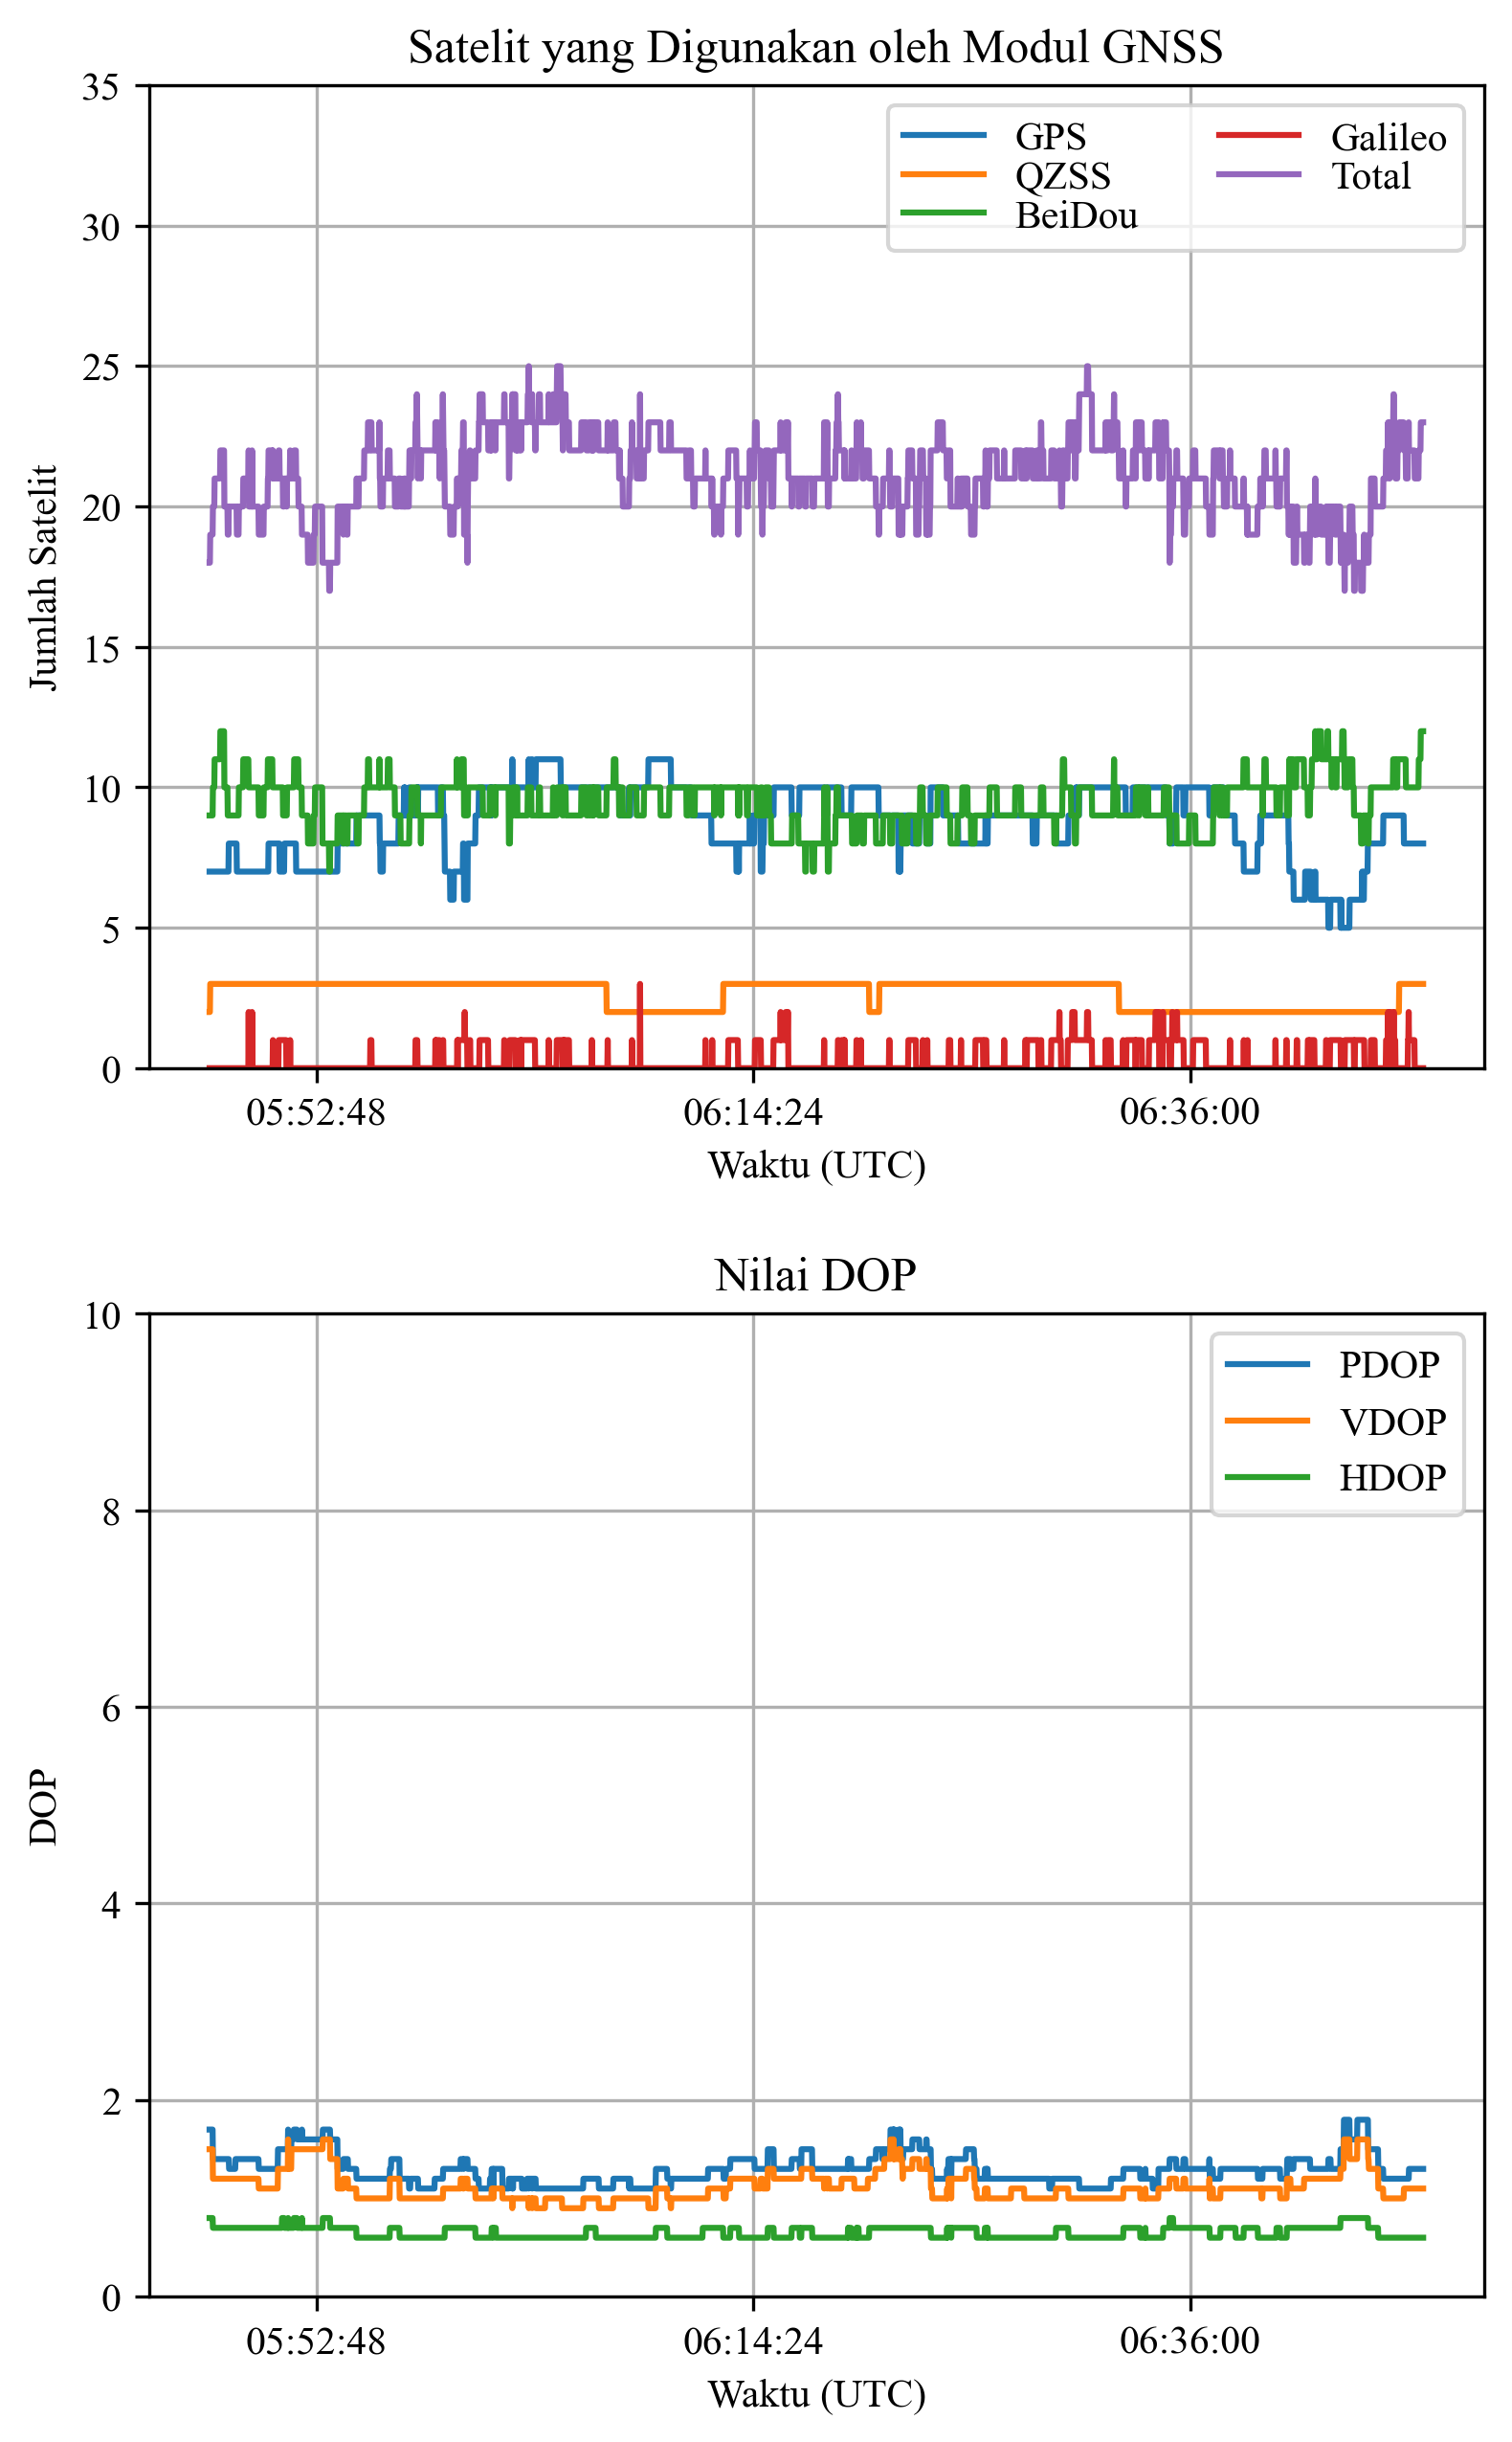
\includegraphics[width=12cm]{contents/chapter-4/4-skenario-outdoor/sats_dop.png}
	\caption{DOP dan Visibilitas Satelit Pengujian Pengujian Ruang Terbuka}
	\label{Fig: outdoor-dop_sats}
\end{figure}

Hasil pengujian menunjukkan bahwa skenario pengujian di ruang terbuka menghasilkan hasil pengukuran yang paling baik dibandingkan dengan tiga pengujian sebelumnya. Dari pengujian tersebut, didapatkan nilai MAD sebesar 1,21 meter atau sekitar 20\% lebih baik dari nilai yang tertera pada datasheet, yaitu 1,5 meter. Selain itu, jika dibandingkan dengan pengujian semi terbuka, tingkat presisi modul Teseo-LIV3FL meningkat sekitar 60\% dan akurasi bidang horizontal meningkat sebesar 28\%. Hal ini menunjukkan bahwa pengujian di ruang terbuka memberikan hasiil yang lebih baik dan stabil bagi modul GNSS dalam pengukuran. 

\section{Pengujian \textit{Geofencing}}
\subsection{\textit{Geofencing} Wilayan Universitas Gadjah Mada}
\subsection{\textit{Geofencing} Halte Trans Gadjah Mada}

\section{Pengujian di Bus Trans Gadjah Mada}
Pengujian di Bus Trans Gadjah Mada dilakukan untuk meninjau performa sistem dalam keadaan bergerak. Sistem diletakan di dalam kendaraan bus yang terbuat dari logam. Rute pengujian mengikuti rute 1B Trans Gadjah Mada yang dimulai dari Halte Grha Sabha Pramana hingga kembali lagi ke Halte Grha Sabha Pramana dengan durasi waktu satu jam. Peta dari Trans Gadjah Mada Rute 1B ditunjukan oleh Gambar \ref{Fig: peta-1b}.

\begin{figure}[H]
	\centering
	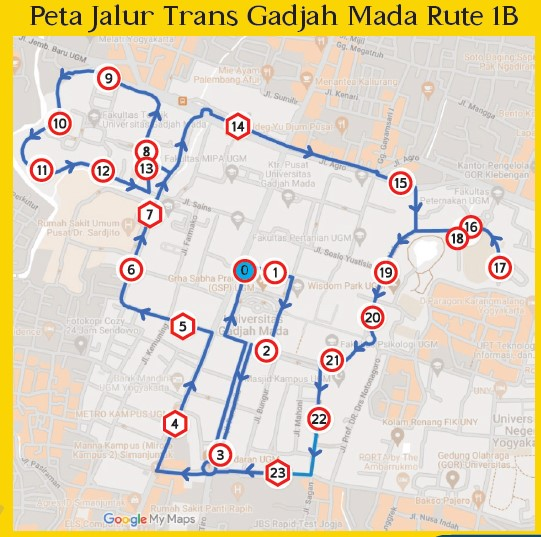
\includegraphics[width=10cm]{contents/chapter-4/pengujian-bergerak/Peta-Jalur-Rute-1B.jpg}
	\caption{Peta Jalur Trans Gadjah Mada Rute 1B}
	\label{Fig: peta-1b}
\end{figure}

Gambar \ref{Fig: moving-dop} menunjukan nilai DOP di setiap titik yang direpresentasikan oleh kode warna di sebelah kanan. Jika warna dari poin semakin mendekati warna merah maka nilai DOP-nya semakin buruk (mendekati 99). 

\begin{figure}[H]
	\centering
	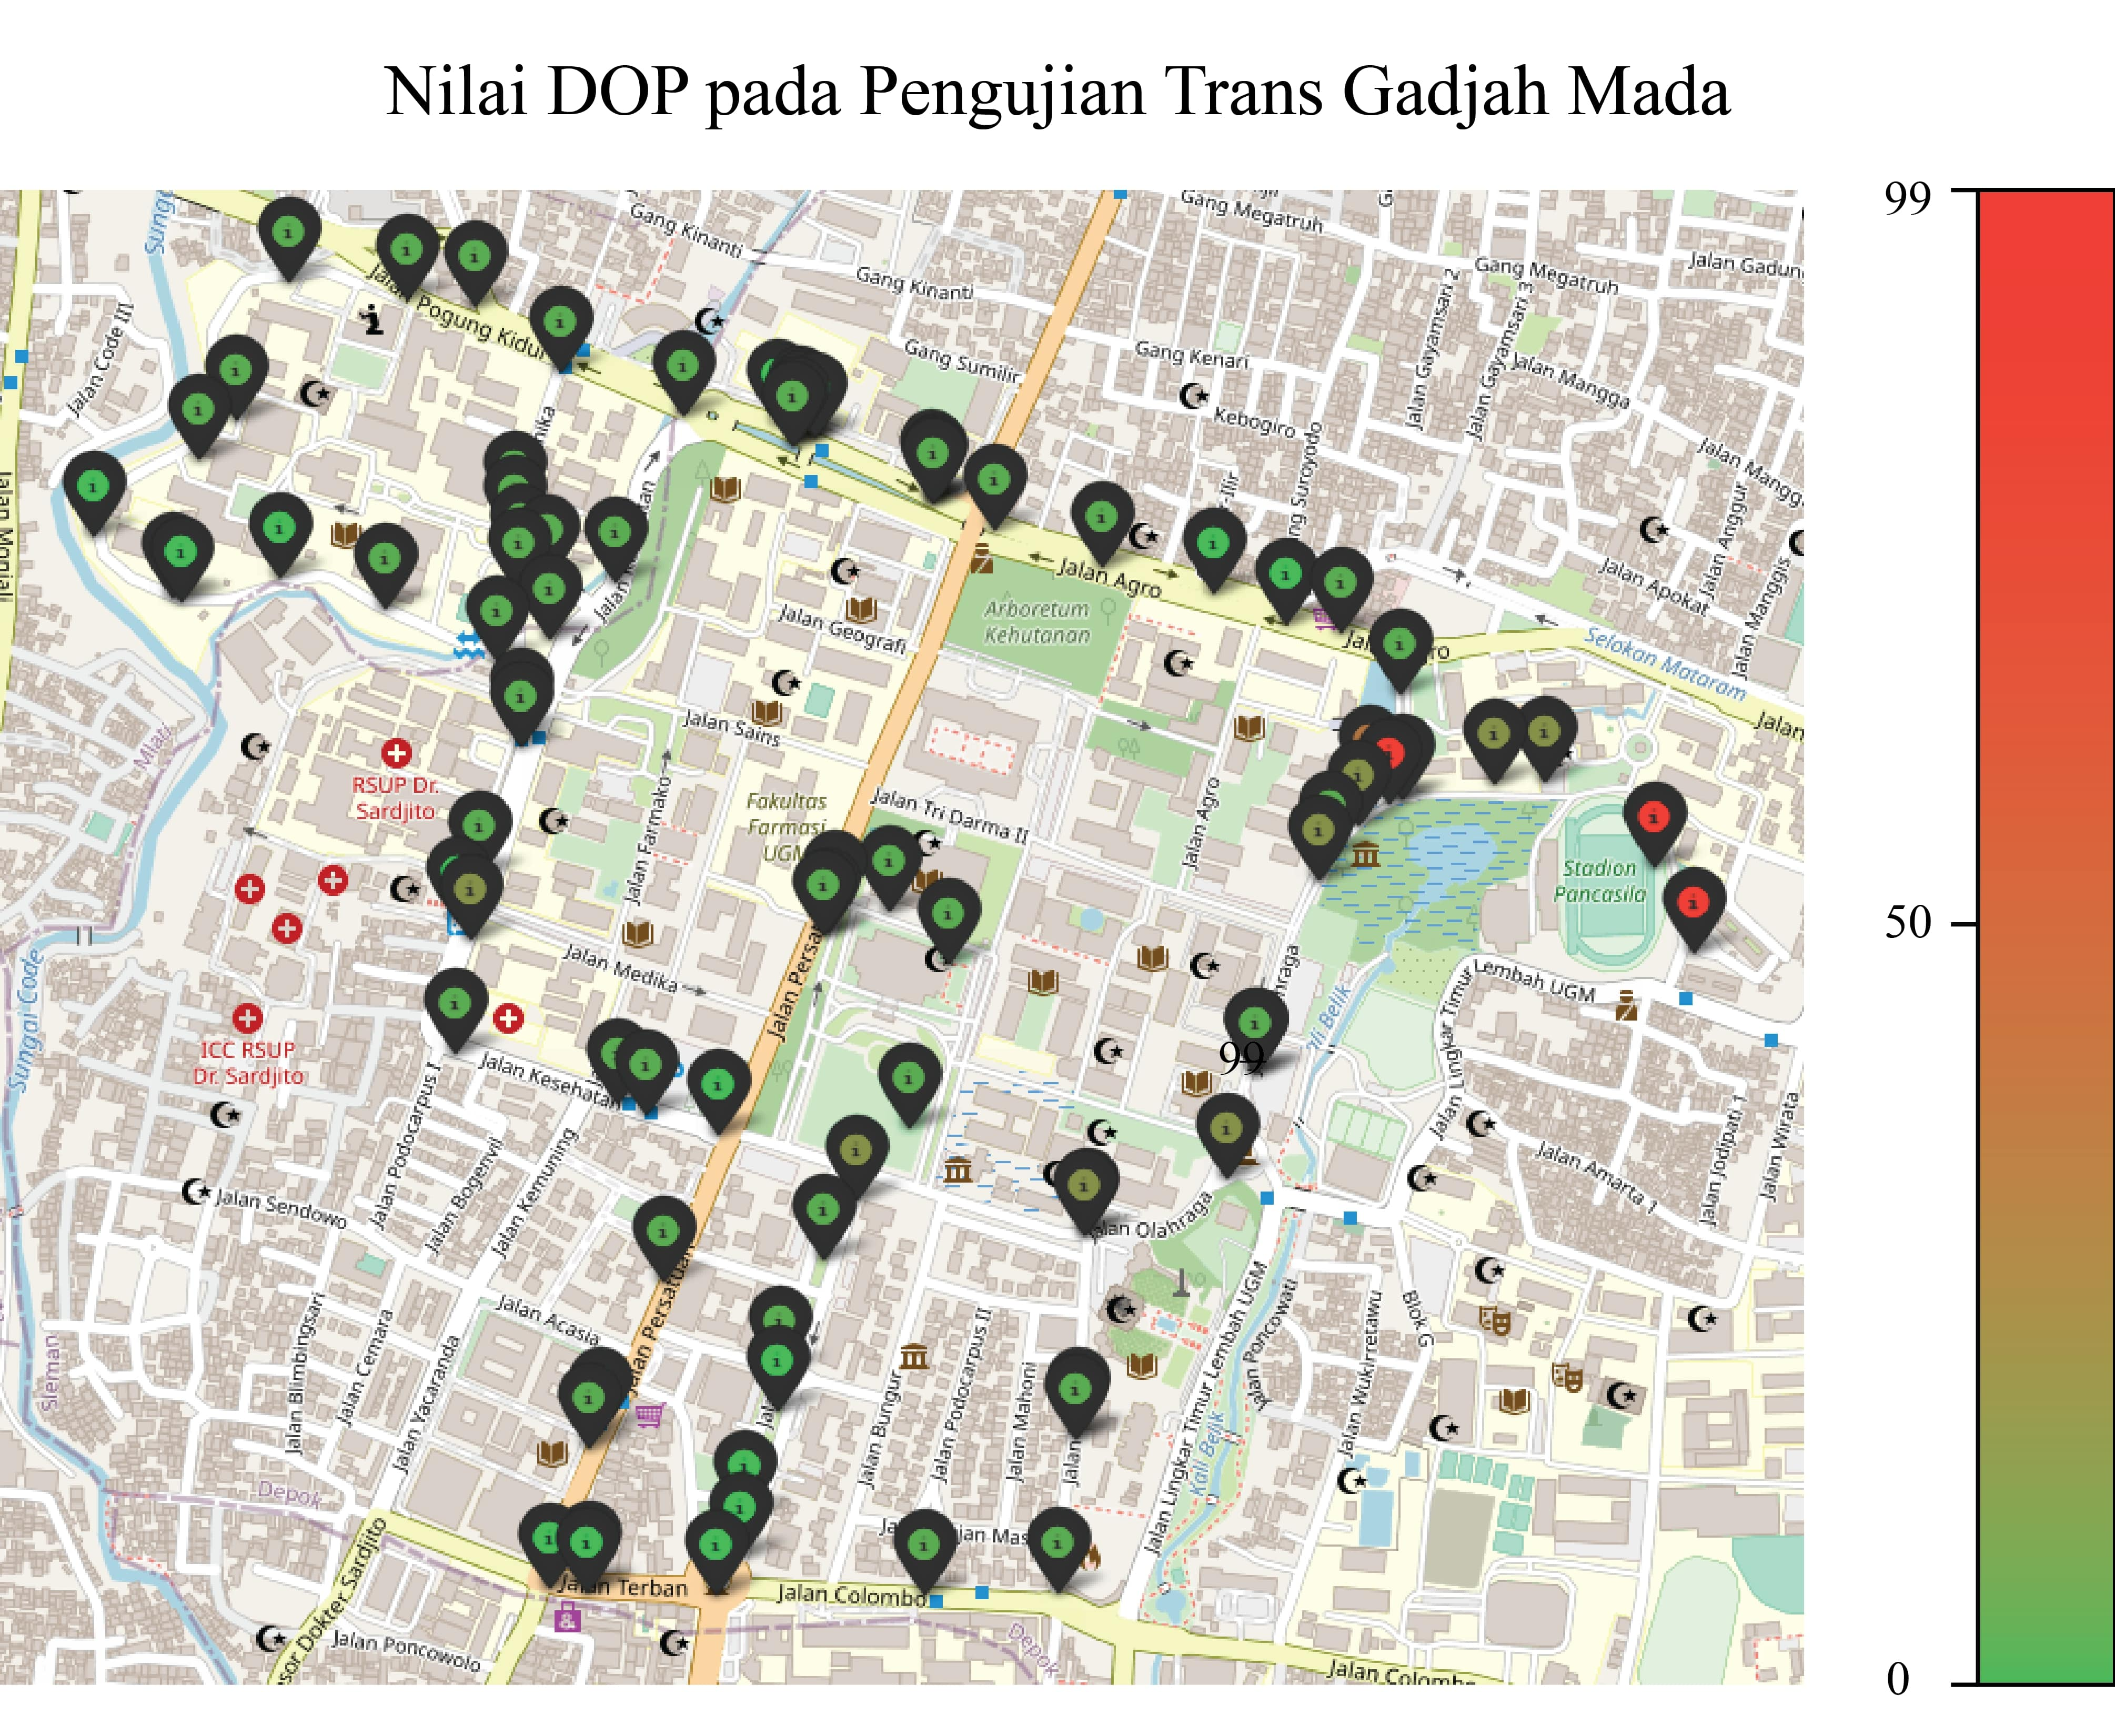
\includegraphics[width=12cm]{contents/chapter-4/pengujian-bergerak/moving-dop.jpg}
	\caption{Pengujian Skenario Dalam Ruangan}
	\label{Fig: moving-dop}
\end{figure}

Terlihat bahwa nilai DOP berada di rentang sangat buruk ketika berada di sekitar Bulaksumur Residence dan Stadion Pancasila. Hal tersebut dikarenakan lingkungan di sekitar pengujian banyak ditutupi oleh pepohonan dan terdapat beberapa gedung seperti ditunjukan oleh Gambar \ref{Fig: lp-streetview}. Halangan-halangan tersebut dapat mengurangi visibilitas dari satelit sehingga mengurangi akurasi dari modul GNSS yang mengakibatkan lonjakan nilai DOP.

\begin{figure}[H]
	\centering
	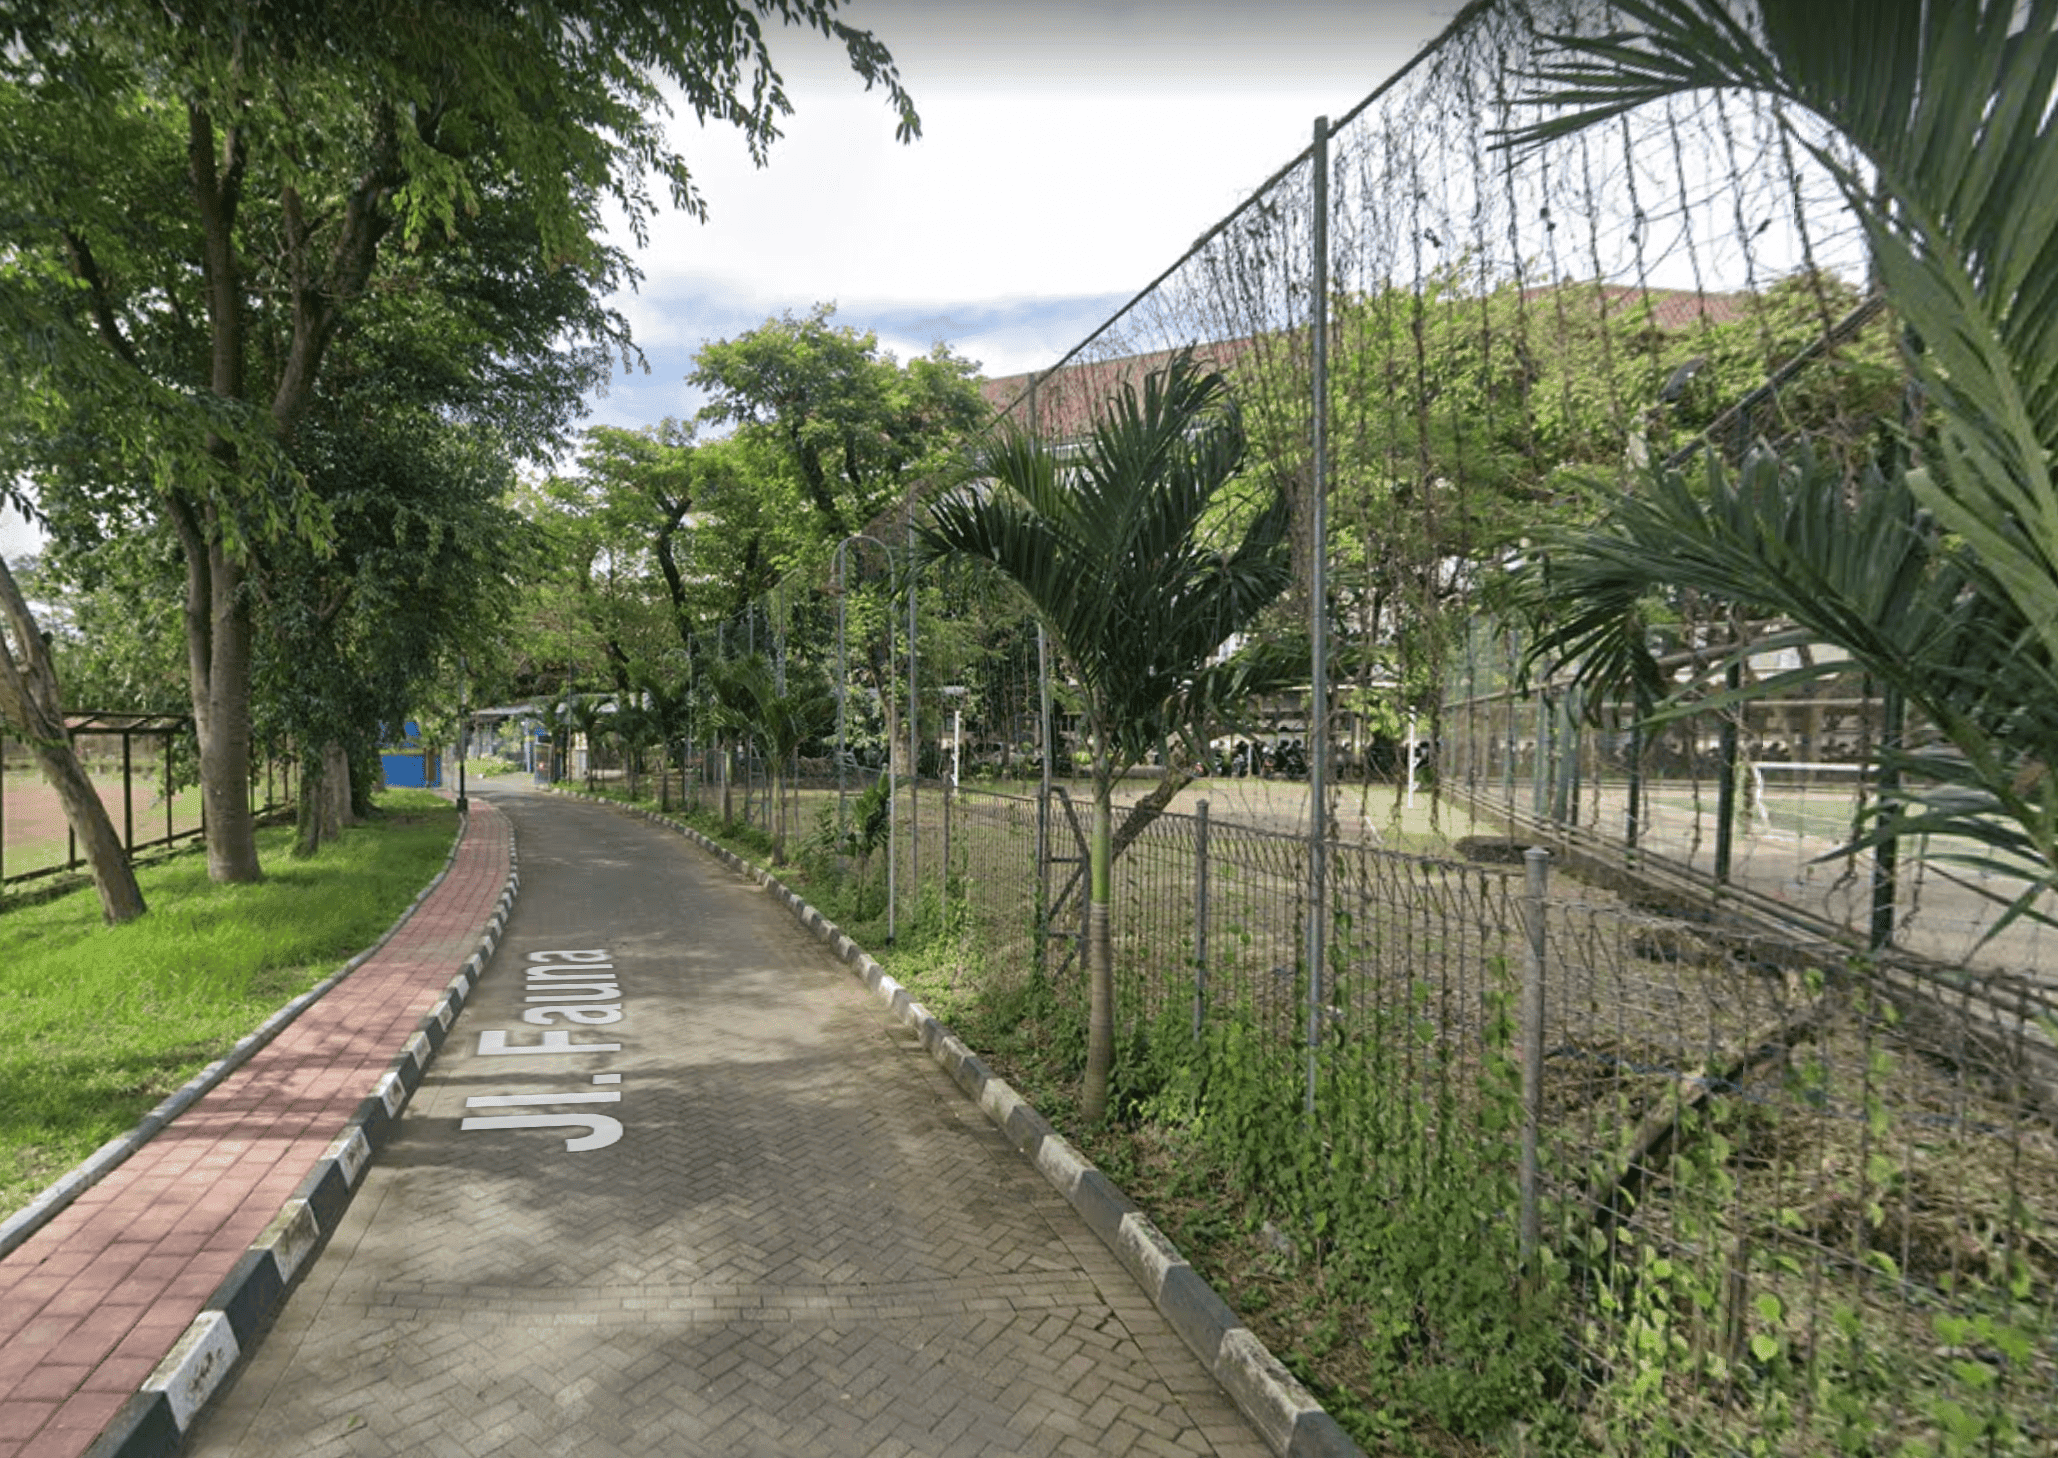
\includegraphics[width=10cm]{contents/chapter-4/pengujian-bergerak/lp-streetview.png}
	\caption{Keadaan di Sekitar Bulaksumur Residence}
	\label{Fig: lp-streetview}
\end{figure}

Visibilitas satelit di setiap titik ditunjukan oleh Gambar \ref{Fig: moving-sats}. Semakin banyak satelit yang digunakan maka warna pada poin akan semakin mendekati warna hijau. Visibilitas satelit terbaik didapat ketika berada di lingkungan Fakultas Teknik, Grha Sabha Pramana, dan Bundaran Universitas Gadjah Mada. Tiga lokasi tersebut memiliki penghalang yang lebih sedikit jika dibandingkan dengan lokasi-lokasi lainnya.

Lokasi dengan visibilitas satelit paling buruk adalah Stadion Pancasila dan Bulaksumur Residence. Gambar \ref{Fig: moving-dop} menunjukan bahwa daerah tersebut juga memiliki nilai DOP paling buruk yang ditandai oleh poin berwarna merah. Terlihat bahwa visibilitas satelit dapat mempengaruhi nilai DOP. Berdasarkan data yang diperoleh, terlihat bahwa lokasi Stadion Pancasila dan Bulaksumur Residence memiliki visibilitas satelit paling buruk dibandingkan dengan lokasi lainnya. Hal ini dibuktikan oleh Gambar \ref{Fig: moving-dop} yang menunjukkan bahwa daerah tersebut memiliki nilai DOP yang paling buruk, yang ditandai oleh poin berwarna merah. Dari gambar tersebut juga dapat dilihat bahwa visibilitas satelit memainkan peran penting dalam mempengaruhi nilai DOP. 

Visibilitas satelit tidak memberikan peningkatan kualitas \textit{fix} yang signifikan ketika jumlah satelit yang digunakan setidaknya lebih dari lima buah satelit. Jika meninjau visibilitas satelit di sekitar RSUP Dr Sardjito, terlihat bahwa visibilitas satelit tidak sebaik di lingkungan Fakultas Teknik, tetapi nilai DOP tetap berada dalam rentang yang cukup baik.

\begin{figure}[H]
	\centering
	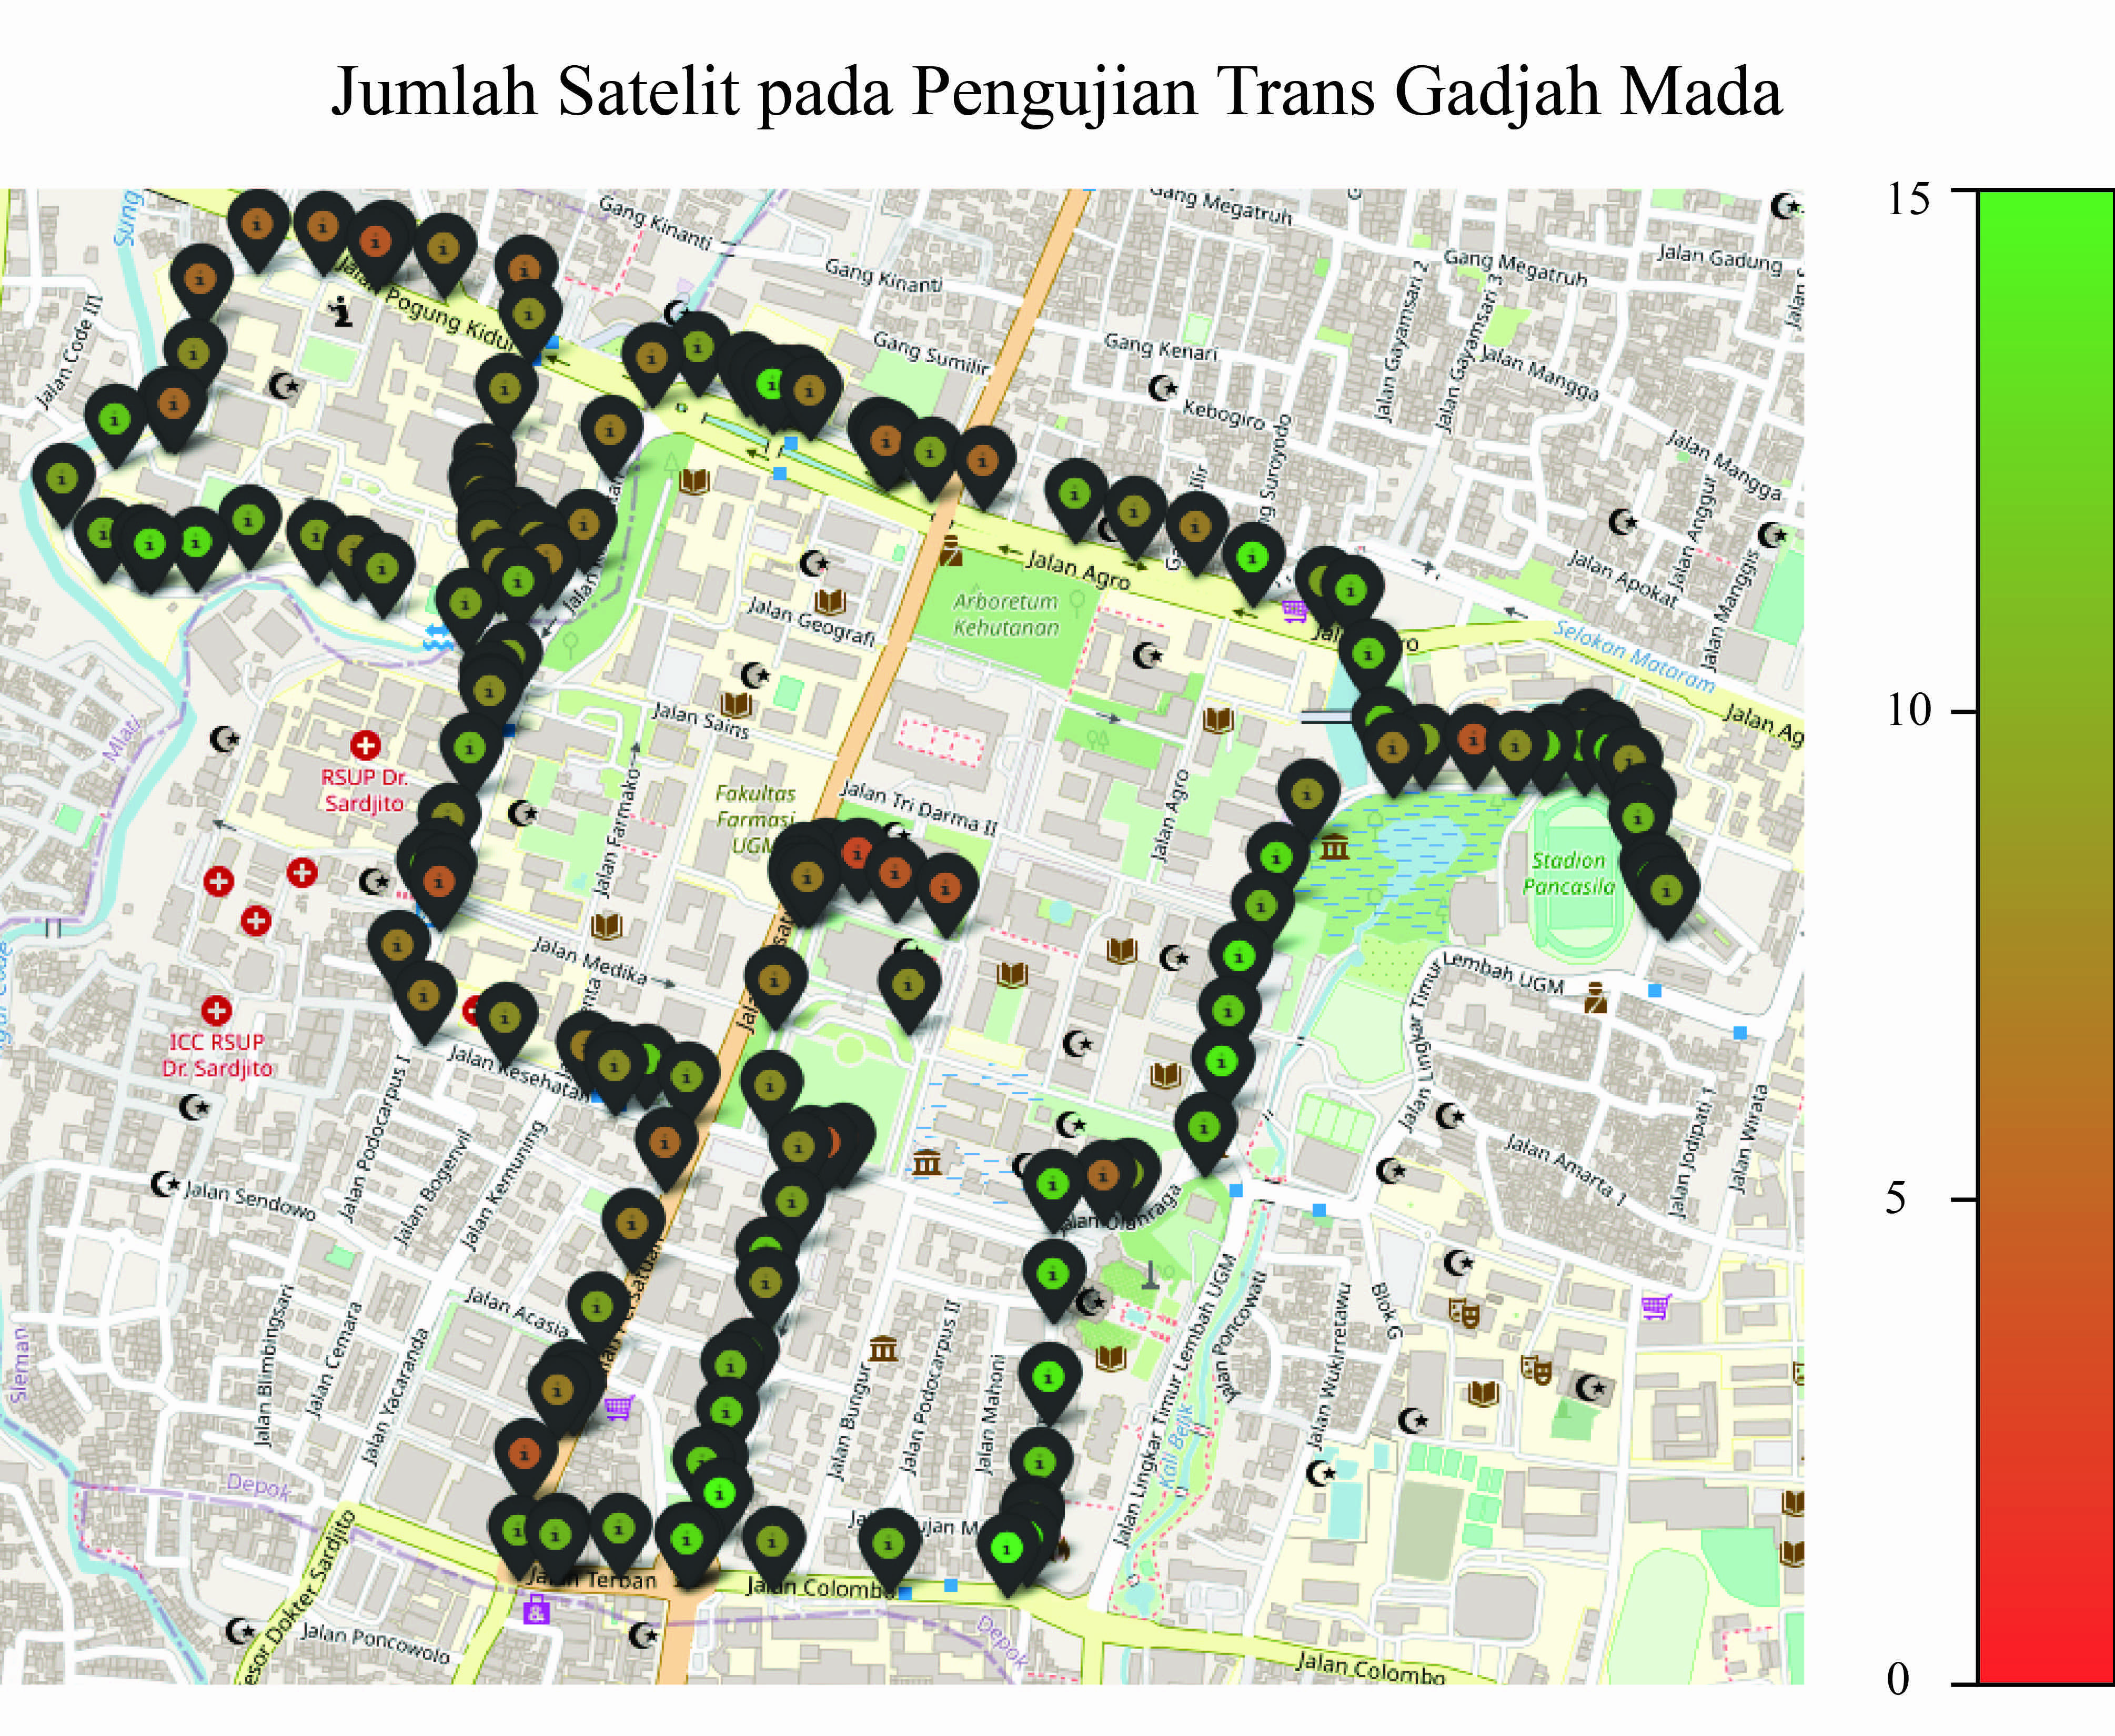
\includegraphics[width=12cm]{contents/chapter-4/pengujian-bergerak/moving-sats.jpg}
	\caption{Pengujian Skenario Dalam Ruangan}
	\label{Fig: moving-sats}
\end{figure}

\chapter{KESIMPULAN DAN SARAN}

\section{Kesimpulan}
Berdasarkan penelitian yang telah dilakukan, dapat ditarik beberapa kesimpulan sebagai berikut:
\begin{enumerate}
	\item Penggunaan multi-constellation pada modul Teseo-LIV3FL dapat memperbaiki performa sistem dalam berbagai kondisi seperti ditunjukan pada pengujian Rapid Static Survey pada skenario basement. Untuk mendapat performa terbaik sistem maka posisi paling idealnya adalah berada di kondisi ruang terbuka dengan halangan seminimal mungkin.
	\item Algoritma mode daya rendah pada modul Teseo-LIV3FL memungkingkan modul untuk bekerja dengan efisien dan dapat digunakan dalam penggunaan jangka panjang. Arus yang mengalir pada modul adalah sebesar 7uA pada mode stand by dan 50mA pada mode akuisisi.
	\item Berdasarkan pengujian secara langsung, firmware dapat melacak posisi Bus dengan baik. Adapun visibilitas satelit yang didapat berada dalam rentang empat s.d. dua belas dan nilai HDOP berada pada rentang 0.4 s.d 2. Meskipun sempat tidak dapat menerima isyarat GNSS di daerah tertentu, sistem dapat melakukan pemulihan dan melanjutkan pelacakan kembali.
\end{enumerate}

\section{Saran}
Adapun saran untuk penelitian lebih lanjut adalah sebagai berikut:
\begin{enumerate}
	\item Perlu dilakukan pengujian lebih lanjut dalam kondisi berbeda seperti kondisi langit tidak ideal ketika cuaca buruk.
	\item Perlu ditambahkan basis data untuk menyimpan data pelacakan dan mekanisme penyimpanan seperti penggunaan REST API.
	\item Untuk mempermudah visualisasi hasil pelacakan Bus dapat dikembangkan sebuah aplikasi yang dapat berjalan di berbagai macam gawai seperti aplikasi berbasis web atau PWA.
\end{enumerate}


%======================================

%======================================
%  References
%======================================
\thereferences
% You can change 
%    the filename and location of the files inputted
\bibliography{references}
%======================================

%======================================
%  Appendix
%======================================
% You can change 
%    the filename and location of the files inputted
\chapterappendix{contents/appendix/appendix}
%======================================

\end{document}